%%____________________________________________________________________________||
\section{Systematic uncertainties in background estimation}
\label{sec:systematics}

This section addresses the estimation of systematic uncertainties
associated with the predictions of the non-multijet backgrounds. Since
this analysis aims to rely as much as possible on the data control
samples to check for sources of bias and derive and/or cross check
systematic uncertainties, a detailed study can only be meaningfully
carried out with data. The strategies that are employed to
ascertain the presence of biases or otherwise, and the procedures used
to derive systematic uncertainties, are described below. 
% Presented
% first are the MC-based
% expectations for uncertainties in the background predictions under the
% assumption of zero bias (\ie, only the statistical component) for the
% $3~\ifb$ scenario. %and $10\ifb$ data scenarios. 
% These studies utilise the
% \ej and \eej control samples that are not yet used in the initial
% data studies. After this, 
A set of closure tests made with $1.28~\ifb$ of certified
data are presented. They are subsequently used to estimate the first
set of systematic errors to be used in the analysis. The assumptions made in 
the projections of physics reach
that are detailed in Sec.~\ref{sec:susy} are also outlined.

Two types of systematic uncertainty are considered separately.
Firstly, we consider
the normalisation uncertainties that affect the background predictions for
the signal region in each (\nb,~\njet,~\scalht) bin (integrated over
\mht).
These uncertainties are estimated with closure tests, described in
Sections~\ref{sec:bkgdnorm-syst} and \ref{sec:syst-from-closure}.

Secondly, systematic effects that may result in the migration of
(simulated) events between \mht bins within a given (\njet~,\nb~,\scalht)
bin are accounted for by providing alternative templates to the nominal
\mht template obtained from simulation. These alternative \mht
templates may be derived from, or at least cross checked with, the
data control samples, as described in Sec.~\ref{sec:syst-on-shape}.

% % Maybe we can re-use this table at some point
% \begin{table}[h!]
%   \caption{Systematic uncertainties on the transfer factors as a
%     function of \scalht.}  
%   \label{tab:bkgd-syst}
%   \setlength{\extrarowheight}{2.5pt}
%   \centering
%   \begin{tabular}{ llccc }
%     \hline
%     \hline
%     \scalht region [GeV] & 200-600 & 600-1000  & $>1000$  \\ 
%     \hline
%     Uncertainty [\%] & 10 & 20 & 30 \\
%     \hline
%     \hline
%   \end{tabular}
% \end{table}
%
% The uncertainties associated with the b-tag ``fomula method'' used
% during Run~1 are ascertained through a dedicated procedure and are
% assumed to be sub-dominant with respect to the \scalht-dependent
% uncertainties derived from the closure tests, as observed during
% Run~1. 
%\clearpage

\subsection{Closure tests}
\label{sec:closure-tests-desc}
\label{sec:bkgdnorm-syst}

The background estimates are determined in each (\nb~,\njet,~\scalht) bin by
defining transfer factors from control region to signal region, as
described in Sec.~\ref{sec:selection}. Since the transfer factors
are obtained from simulation, an appropriate systematic uncertainty is
assigned to each transfer factor to account for limitations in the
simulation modelling of event kinematics and instrumental effects. The
next four sections describe how the systematic uncertainties are
determined from closure tests in data.

The sensitivity of the transfer factors to potential limitations in
the simulation modelling is established through sets of closure tests,
which confront data yields measured in one data control (sub-)sample
against the predictions determined from another data control
(sub-)sample as a function of \scalht. \ie, an extrapolation is made
from one control (sub-)sample to another (rather than to the signal
region) in bins of \scalht via appropriate transfer factors, again
determined from simulation. A large ensemble (\ie hundreds) of
statistically independent closure tests are performed between a number
of control (sub-)samples to identify any potential sources of bias in
the transfer factors.

The level of statistical consistency between the predicted and
observed yields of each closure test in the ensemble is inspected, in
the absence of any bias in the transfer factors. The level of
agreement between the predicted and observed yields is expressed as
the ratio $(\nobs - \npre)/\npre$ while considering only the
statistical uncertainties on \npre and \nobs. Therefore, the level of
closure is defined by the statistical significance of a deviation in
the ratio from zero. A set of closure tests includes ratios determined
for each \scalht bin. In this way, a set of closure tests allows one to
establish the presence of significant biases or otherwise, and any
possible dependence on \scalht. If statistically significant biases
are observed, further studies are required to understand and correct
for these biases.

Under the assumption of closure for the full ensemble of tests,
systematic uncertainties on the transfer factors are derived for each
\njet and \nb~category and \scalht bin. The treatment for
estimating the systematic uncertainties on the transfer factors is
described in Sec.~\ref{sec:syst-from-closure}.

In the case that there are no statistics in a control region (sub-)sample
to perform one of the closure tests, the bin in question would not be 
used in the statistical interpretation of the analysis.


\subsection{Systematic uncertainties in the transfer factors\label{sec:syst-from-closure}}

Once it is established that no significant bias or trend is observed
for any set of closure tests, the systematic uncertainties associated
with the transfer factors are determined. The statistical precision of
the closure tests is considered a suitable benchmark for determining
the systematic uncertainties that are assigned to the transfer
factors, as it is only the statistical uncertainties associated with
the tests that limit our knowledge of whether closure is actually
achieved or otherwise.

The systematic uncertainties in the transfer factors can be considered
as a ``normalisation'' uncertainty in the SM background predictions,
which are determined per \scalht bin per (\njet,~\nb) category and are
assumed to be fully uncorrelated between the different (\njet,~\nb)
categories and \scalht bins. Further details are provided in Section
\ref{sec:likelihood}. 

The systematic uncertainty is estimated by taking the quadrature sum
of the weighted mean and (square root of) sample variance for the
closure tests within the given \scalht bin. To find ``expected
systematics'', \nobs and \npre are taken from the same MC
(this guarantees closure) but the statistical errors are from the
unweighted and weighted counts respectively. The expected systematic
uncertainty is then taken as the weighted mean of the error on the
closure tests. This is an estimator of the expected variance, assuming
no bias is found in data. 

It is worth noting that we expect a dependence on integrated
luminosity. This is a
reflection of the fully statistical nature of the ``systematic'' in
the absence of bias. 

A missing entry implies that the statistics were
insufficient to complete the necessary set of closure tests and the
\scalht bin is not used for this (\njet,\nb) category. 

%% b jet multiplicity categories and also the seven \scalht regions,
%% which is a conservative approach given that one can expect some
%% correlation between adjacent \scalht bins (due to comparable
%% kinematics). This approach of decorrelating the \scalht regions
%% should be contrasted against the fits that do assume a correlated 
%% behaviour in \scalht.

\subsection{Splitting up the closure tests based on background
processes \label{sec:closure-split}}

One approach for deriving a prediction of the normalisation systematic
on the SM background predictions is to derive one systematic per bin
for all the transfer factors (of which there is one per background process). This is the 
method described in Sec.~\ref{sec:closure-tests-desc}.

An alternative approach would be to split the closure tests based on
the background processes that they are most relevant to. This
allows for the derivation of different systematic errors for different
transfer factors in the same bin.

For this alternative, the closure tests are split into
two sets, those relevant to the $W$ and \ttbar background and those relevant
to the \znunu backgrounds. The closure tests used and motivated in
Sec.~\ref{sec:closure-data-study} are split appropriately between the
two sets. 

At the current stage of the analysis the systematics quoted are only
made from split sets of closure tests in multi-jet bins above
$\scalht>400\gev$. 

\subsection{Closure tests with $1.28~\ifb$ of data}
\label{sec:closure-data-study}

Each set of closure tests should demonstrate in data, within the
statistical precision of each test, that there are no significant
biases or dependencies on \njet nor \scalht inherent in the transfer
factors obtained from simulation. 
% The MC-based studies shown above
% close by construction, but provide information on the precision at
% which biases can be probed, \ie they provide lower bounds on the
% systematic uncertainties that can be derived (described below), which
% can be interpreted as a systematic uncertainty limited by statistical
% uncertainties associated with the data (and simulation).

For the first look at data, the $\ej$ and $\eej$ control samples are
not used. An $\mht>130\gev$ requirement is also made. As the muon
control samples do not have an \alphat cut and \mht is correlated to
\alphat this cut reduces the potential problems
caused by the extrapolation inherent in using low \mht event counts to
predict high \mht event counts.
% Given this fact, and the fact that fewer events are
% available in the $1.28\ifb$ than in the $3\ifb$ MC study a smaller
% subset of closure tests is chosen. Any closure tests utilising the
% electron samples are removed and tests that were carried out
% multiple times with different numbers of b-tags are collapsed into one
% (such as the $\mj\rightarrow\mmj$ tests). 
The set of tests used for
this data study can be seen in the legends of
Fig.~\ref{fig:exampleClosures}.

The $0$ b-tag $\rightarrow1$ b-tag and $1$ b-tag $\rightarrow2$ b-tag
tests probe the
sensitivity of the transfer factors to the relative admixture of
events from the $W$ + jets and \ttbar processes by varying the number
of b-tagged jets within the \mj sample. These tests are conservative,
as the admixture changes little between the \mj sample and the signal
region (as there is no extrapolation in \nb), whereas the closure
tests use sub-samples with different \nb bins and therefore different
admixtures of $W$ + jets and \ttbar events. \eg, the former uses a
$W$-enriched sub-sample (selected by requiring zero b-jets) to predict
yields in a \ttbar-enriched sub-sample (selected by requiring one
b-jet).  These two tests also probe the modelling of the
reconstruction of b-quark jets, although this is addressed more
precisely by dedicated studies involving varying the uncertainties in
b-tag scale factors, as the one performed in the previous analysis,
see for instance \cite{CMS_AN_2013-366}. This study will be repeated
for this analysis in the future.

The \mj $\rightarrow$ $\gamma$ + jets tests deal with
the consistency of the prediction of \wej with $\gamma$ + jets. This is 
important for understanding
the consistency of the \znunu + jets background predictions from both
\wej and \gj events along with the associated assumptions (such
as the negligible effect of the vector boson mass on kinematic
distributions from the V + jets and \gj samples under sufficient
boost). 
% Additional checks between these two sub-samples (and also
% between the single and di-lepton sub-samples) will also be performed
% with the charge of the single lepton sample taken into consideration,
% which will allow to probe the simulation modelling of acceptance
% effects due to $W$ polarisation.

The \mj \rightarrow \mmj tests address the modelling of vector boson production
(including the handling of contamination from \ttbar). The muon
trigger and reconstruction efficiencies are also probed, given that
exactly one and two muons are required in the two control
samples. However, dedicated data-driven methods are used to measure
the muon trigger and reconstruction efficiencies, with values taken
from the muon POG.

The \mmj \rightarrow \gj tests deal with the
consistency between the \zee + jets and $\gamma$ + jets
samples, which is a further check on the validity of using the \gj
process to predict the \znunu\, + jets process.

The $\njet=2\rightarrow\njet=3$ and $\njet=4\rightarrow\njet\geq5$ tests 
probe the simulation modelling of jet
multiplicity in the \mj,
\mmj and \gj samples,
which is checked due to the exclusive binning in jet multiplicity.  As
in the case of the $W$ + jets / \ttbar admixture, these sets of tests
are a conservative check, as predictions are always made from the same
jet multiplicity bin, whereas the closure tests translate between the
two bins.
% Most of these closure tests have been motivated in
% Sec.~\ref{sec:closure-mc-study}, with a few exceptions. 

Additionally, to test the prediction of \znunu + jets processes with
the $W$-enriched \mj control sample, we introduce the
$\mu^{+}\rightarrow\mu^{-}$ closure test, as mentioned in
Sec.~\ref{sec:backgroundmet}. The production mechanism of $W$ from pp collisions means
high $p_T$ $W$ bosons are predominantly left handed \cite{WPol}.  
For high $p_T$ bosons, this implies that $W^+$ decays 
to the left handed neutrino along its direction of motion while 
the lepton is pointing backward. The opposite behaviour is
expected for the $W^-$. The lepton is therefore more boosted (and
the neutrino less boosted) in $W^+$ decays than $W^-$ decays.  This
leads to a larger number of $W^+$ decays in the single lepton control
regions (which relies on the lepton $p_T$ for acceptance) than in the
signal region (which relies on the neutrino $p_T$ for acceptance). The
new closure test checks if this leads to a bias in the prediction of the 
\znunu + jets background. This is discussed in
Appendix~\ref{app:zInvBgControl} and study of this test performed on the
$8\tev$ data is presented.

%%%%%%%%%%%%% FIXME %%%%%%%%%%%%%
% write something about the TT->TL test

The aforementioned closure tests are not the only ones considered or
checked, \ie, the list above is not exhaustive. However, they are a
representative set that cover the main potential sources of bias in
the transfer factors derived from simulation. 

The closure tests are performed for each of the different jet
categories. In Fig.~\ref{fig:closureDataSym} are the results of the
closure tests performed on events in the ``symmetric'' jet category
and in Fig.~\ref{fig:closureDataAsym} the results of the closure tests
performed on events in the ``asymmetric'' jet
category. For events in the ``mono-jet'' category, the closure tests
that rely on more than one jet (such as the $1 b-tag\rightarrow\geq 2
b-tag$ tests) are removed. The results of these tests are in
Fig~\ref{fig:closureDataMono}.

Prior to deriving uncertainties, each individual set of closure tests
(as a function of \scalht) have been inspected for closure. Zero and first order
polynomial fits are performed along the \scalht dimension for each set
of closure tests per jet category. The fits are inspected for any
indication of bias averaged over \scalht as well as any
\scalht-dependant bias.

In the case of the closure tests presented in this section, there are
no tests which demonstrate a significant departure from closure. One
effect that is visible, however, is the lack of b-tag scale factors.
Simulated events are reweighted when these scale factors become
available, but for now we notice a slight defecit in the number of
b-tags observed than predicted. This is manifest in the $0 b-tag
\rightarrow 1 b-tag$ and $1 b-tag \rightarrow \geq 2 b-tag$ closure
tests, that exhibit consistently negative values. We expect this to
improve with the application of the scale factors. 

%%%%%%%%%%%%%%%%%%%%%%%%%%%%%%%%%%%%%%%%%%%%%%%%%%%%%%%%%%%%%%%%%%%%%%%
% representative collections of tests
%%%%%%%%%%%%%%%%%%%%%%%%%%%%%%%%%%%%%%%%%%%%%%%%%%%%%%%%%%%%%%%%%%%%%%%

\begin{figure}[h!]
  \begin{center}
    \subfigure[$\njet =
    1$]{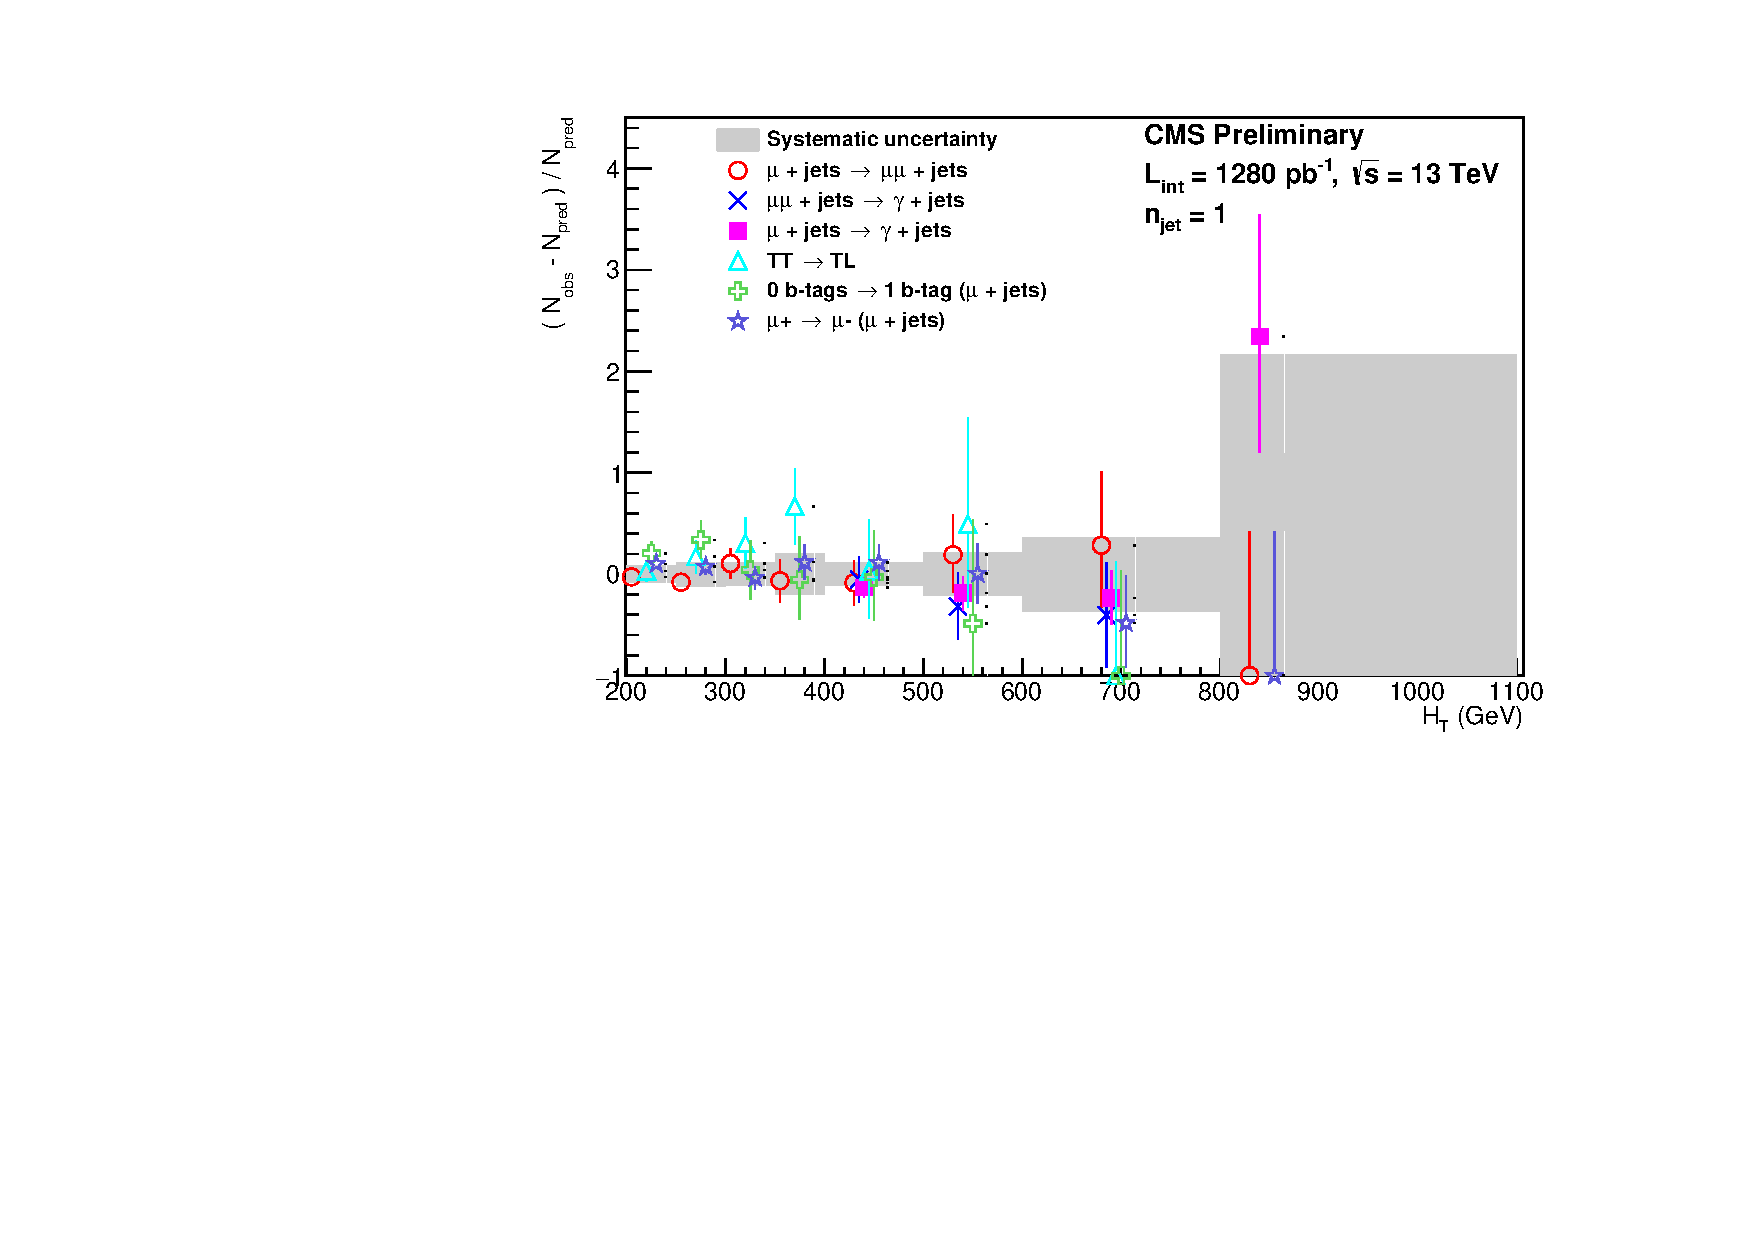
\includegraphics[width=0.5\textwidth]{figures/closureTests/newJamboree/all_eq1j.pdf}} ~~
    \subfigure[Asymmetric $\njet =
    3$]{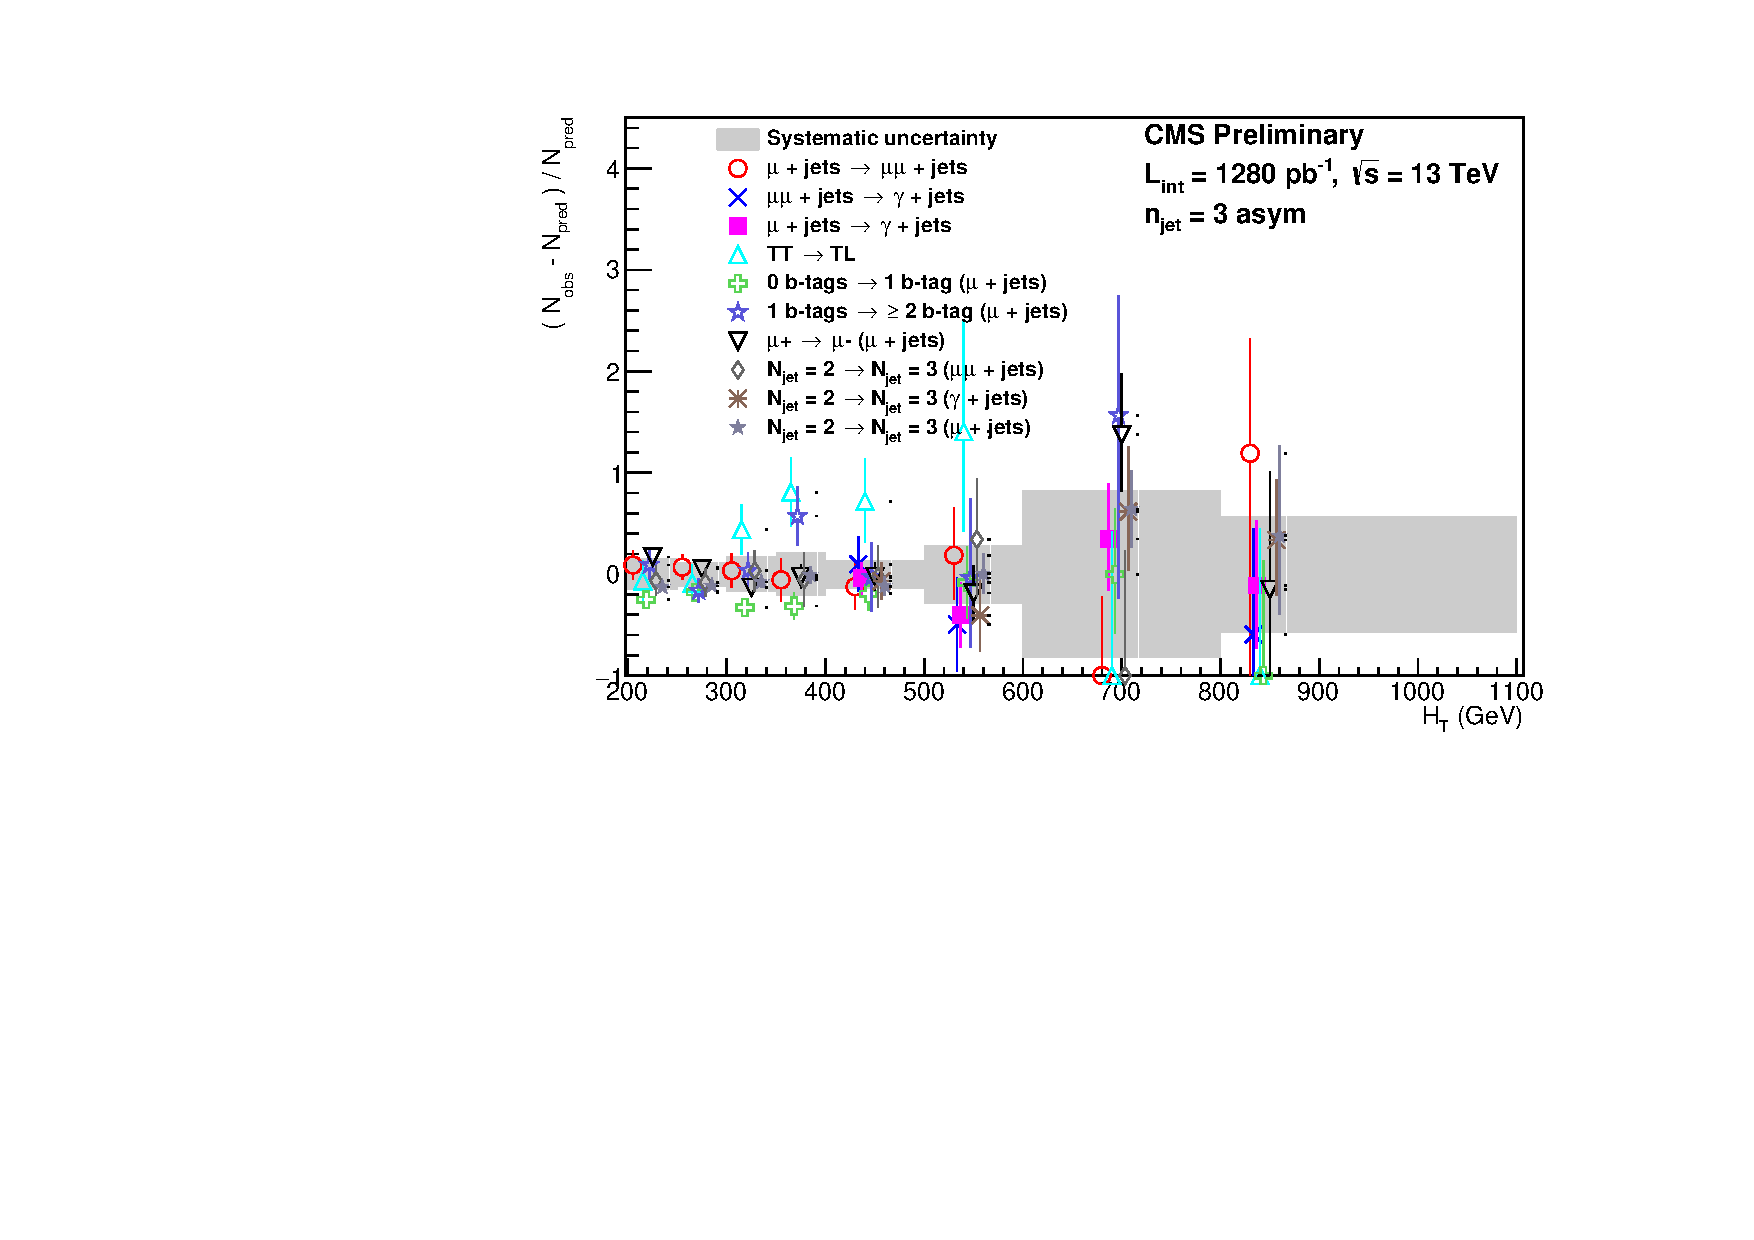
\includegraphics[width=0.5\textwidth]{figures/closureTests/newJamboree/all_eq3a.pdf}} \\
    \subfigure[Symmetric $\njet = 2$ for \znunu closure tests
    ]{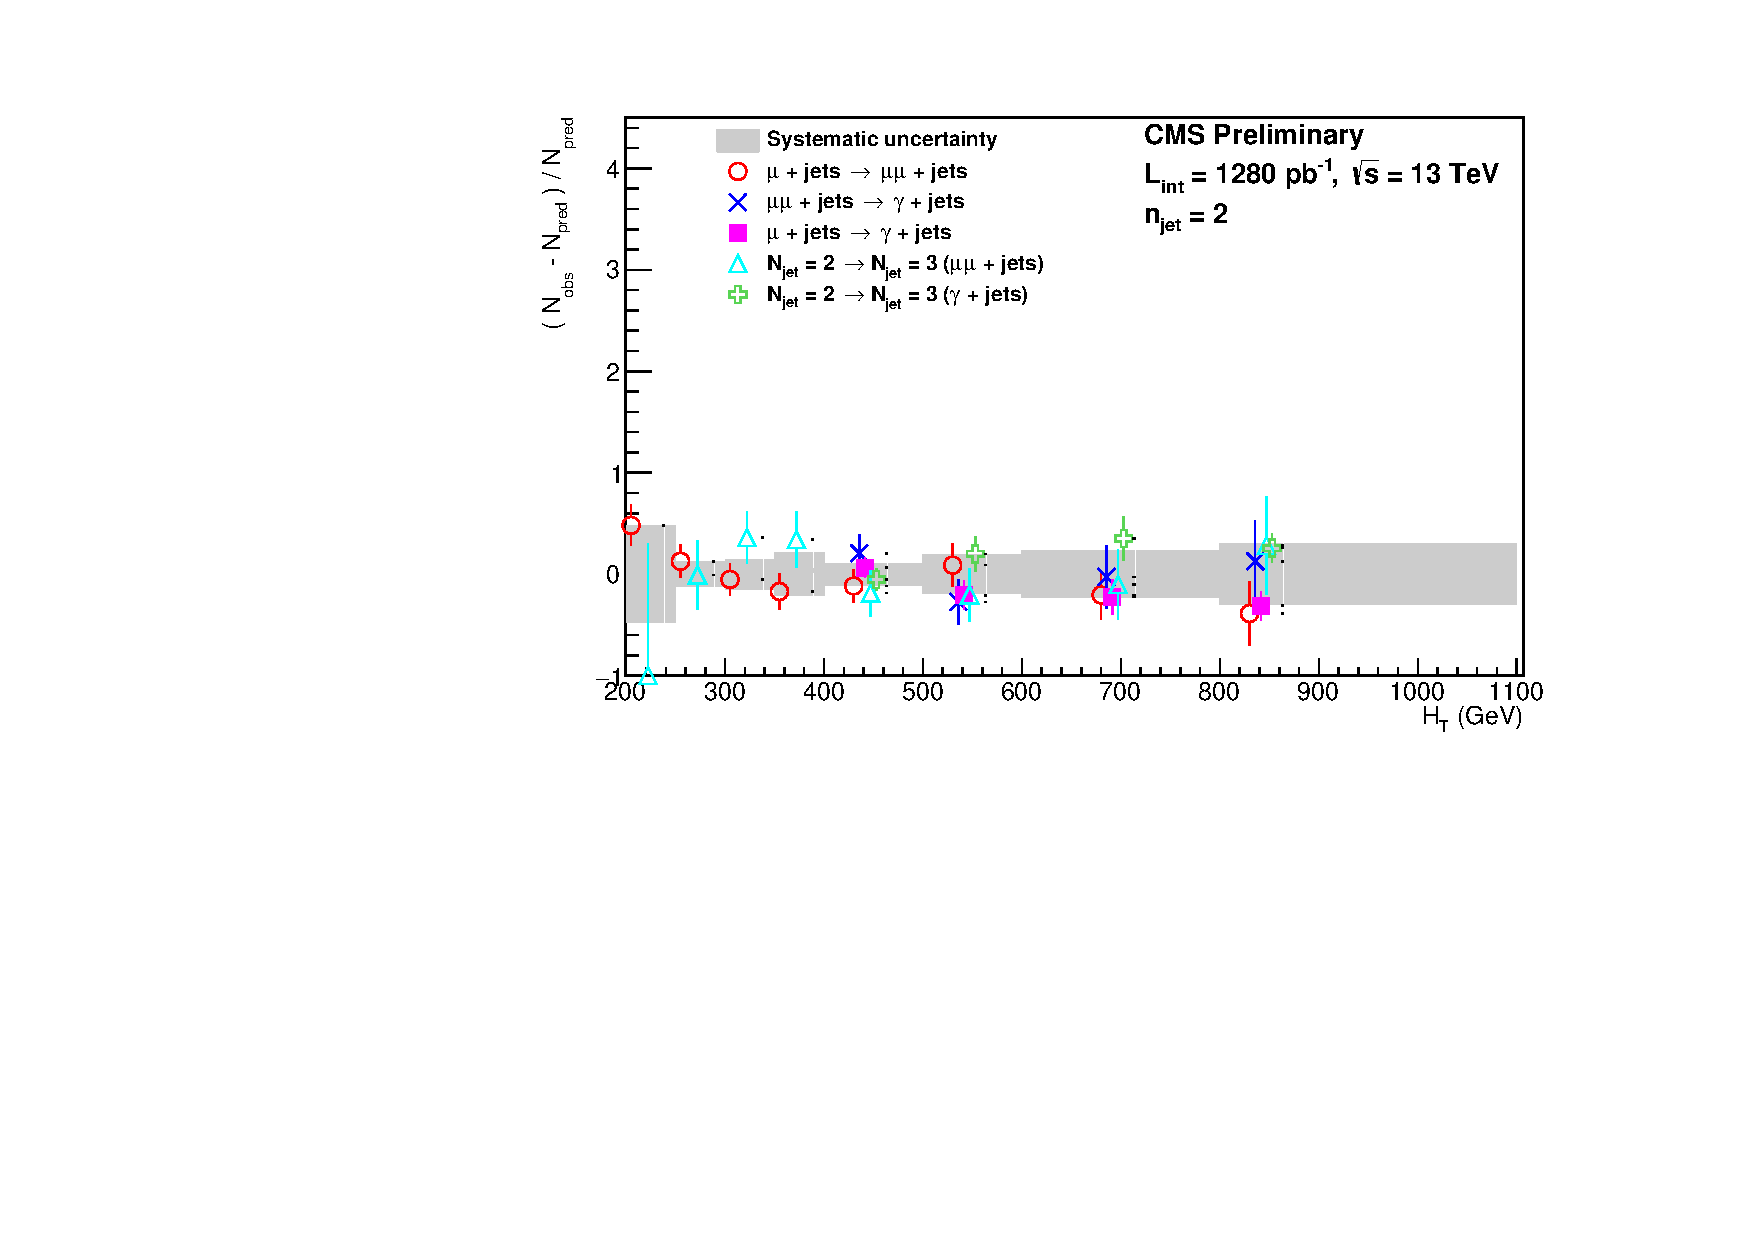
\includegraphics[width=0.5\textwidth]{figures/closureTests/newJamboree/zinv_eq2j.pdf}} ~~
    \subfigure[Symmetric $\njet = 2$ for W and \ttbar + jets closure tests
    ]{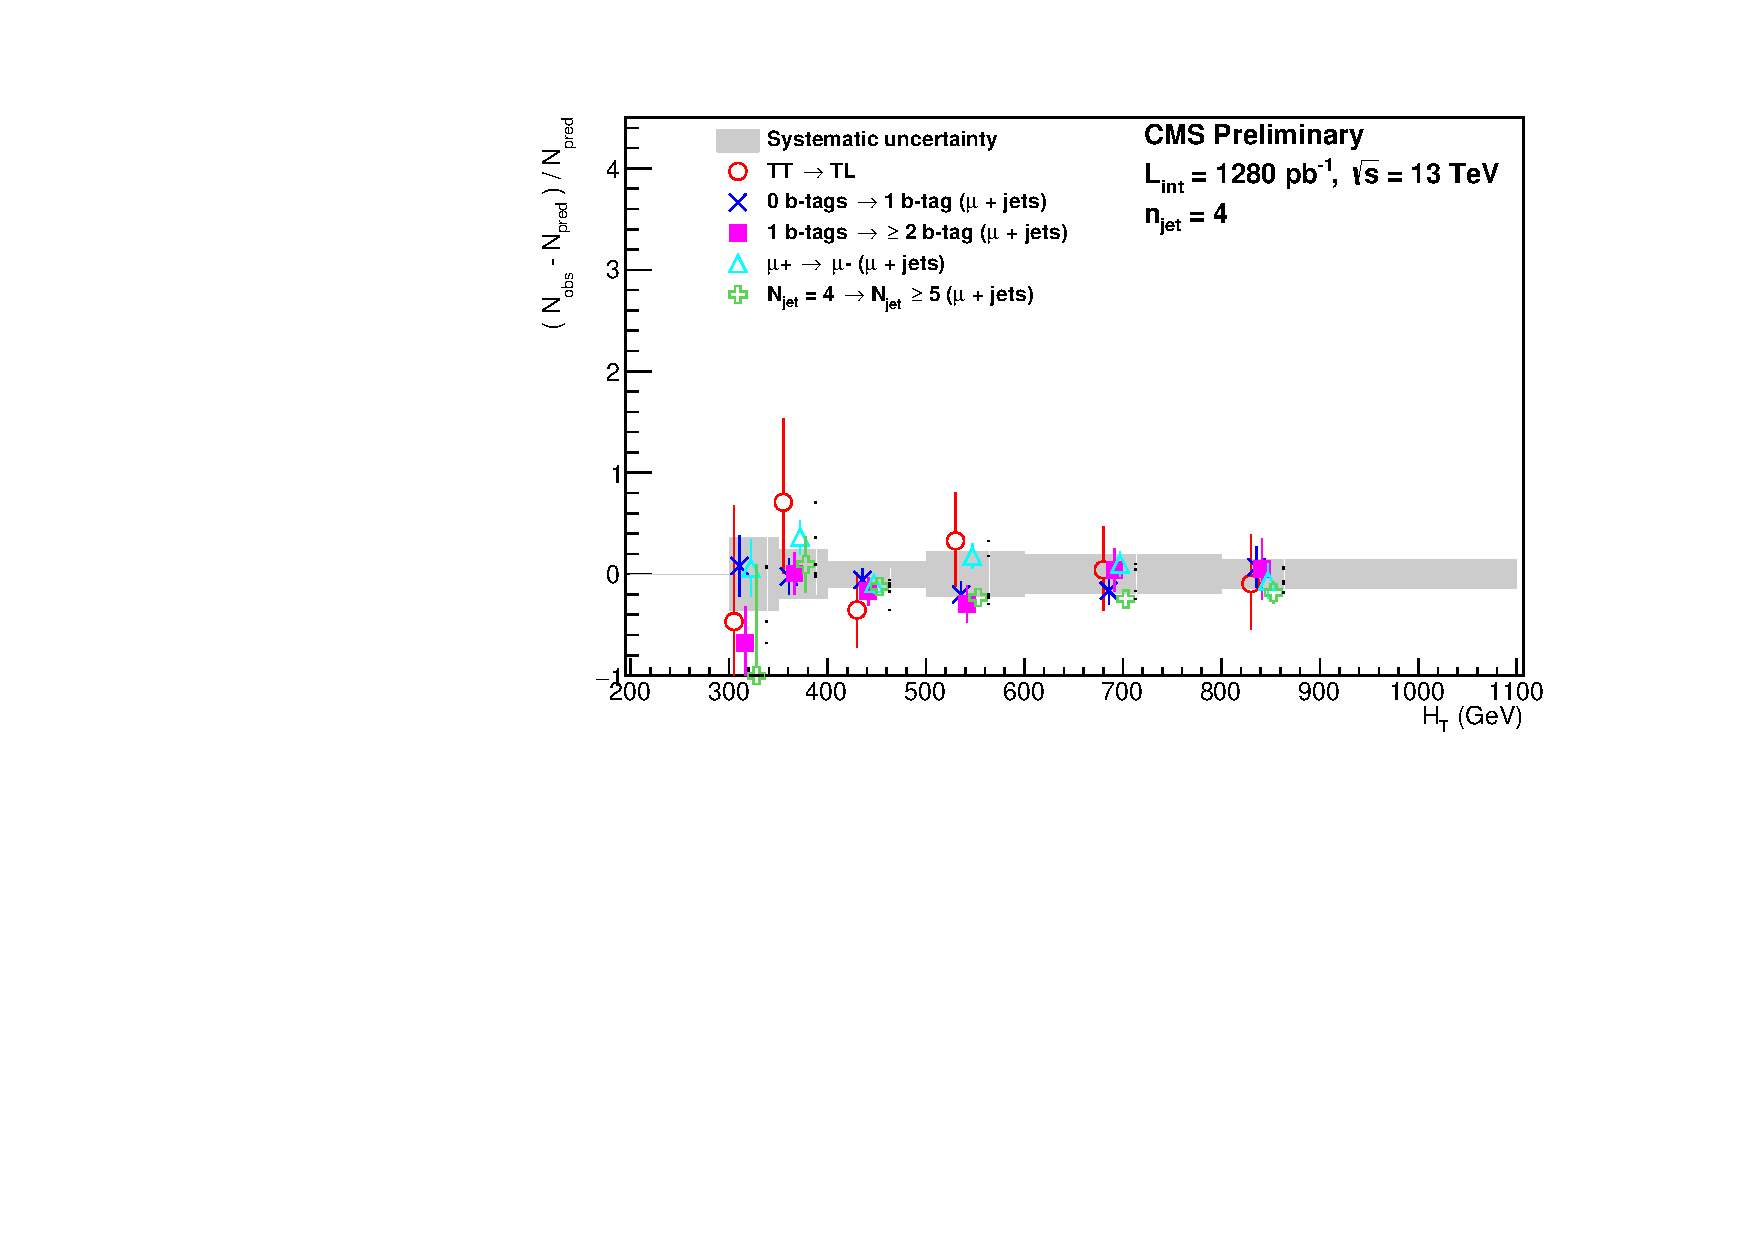
\includegraphics[width=0.5\textwidth]{figures/closureTests/newJamboree/ttW_eq4j.pdf}} \\
    \caption{Examples of closure tests (open symbols) designed to
    probe assumptions made in the background predictions of the
    analysis. These are carried out with $1.28\ifb$ of $13\tev$ data. 
    Closure tests for the mono-jet category are displayed, along with
    examples of ensembles for testing the multi-jet categories. A
    demonstration of ensembles split for the \znunu and W and \ttbar +
    jets closure tests are also included.
    }
    \label{fig:exampleClosures}
  \end{center} 
\end{figure}


%%%%%%%%%%%%%%%%%%%%%%%%%%%%%%%%%%%%%%%%%%%%%%%%%%%%%%%%%%%%%%%%%%%%%%%
% old collections of tests
%%%%%%%%%%%%%%%%%%%%%%%%%%%%%%%%%%%%%%%%%%%%%%%%%%%%%%%%%%%%%%%%%%%%%%%


% \begin{figure}[h!]
%   \begin{center}
%     \subfigure[$\njet =
%     2$]{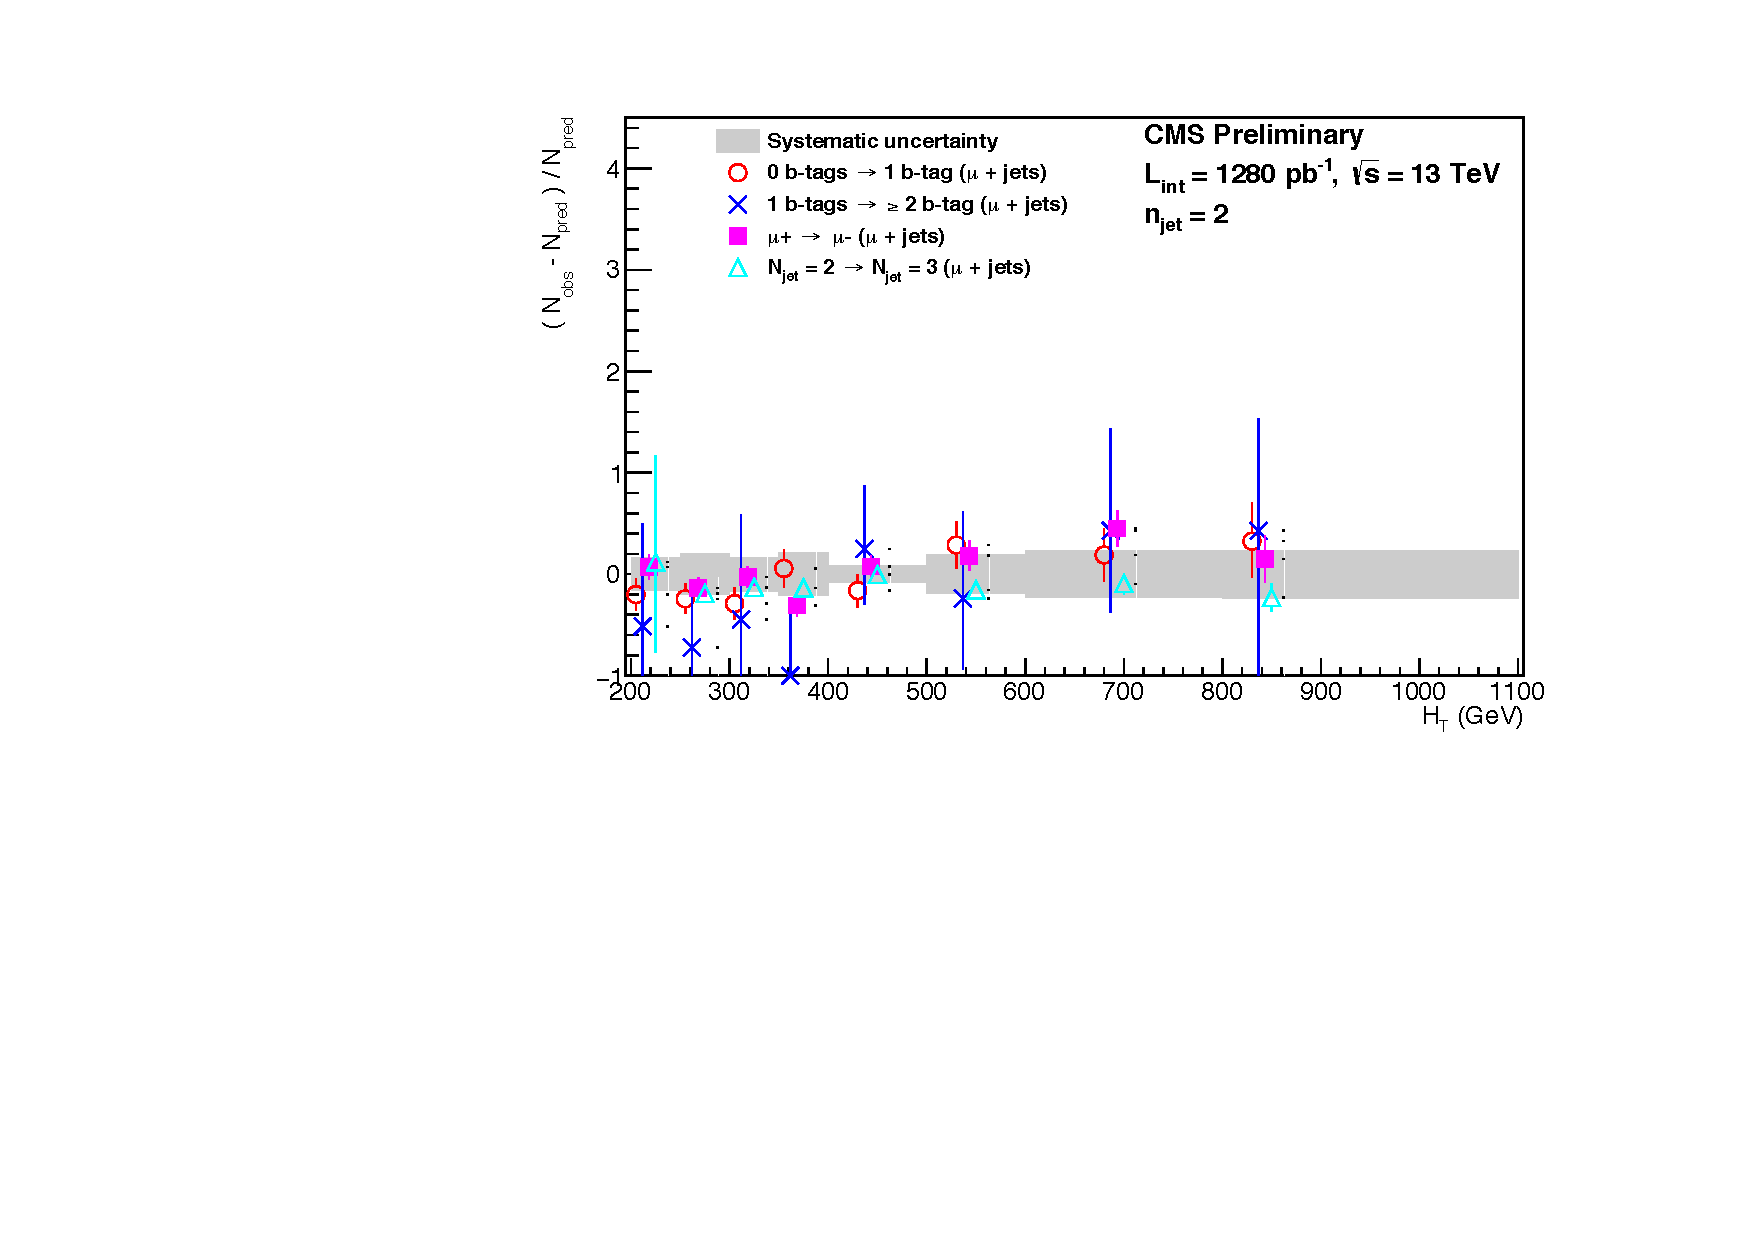
\includegraphics[width=0.5\textwidth]{figures/closureTests/1280pb/ttW/eq2j.pdf}} ~~
%     \subfigure[$\njet =
%     3$]{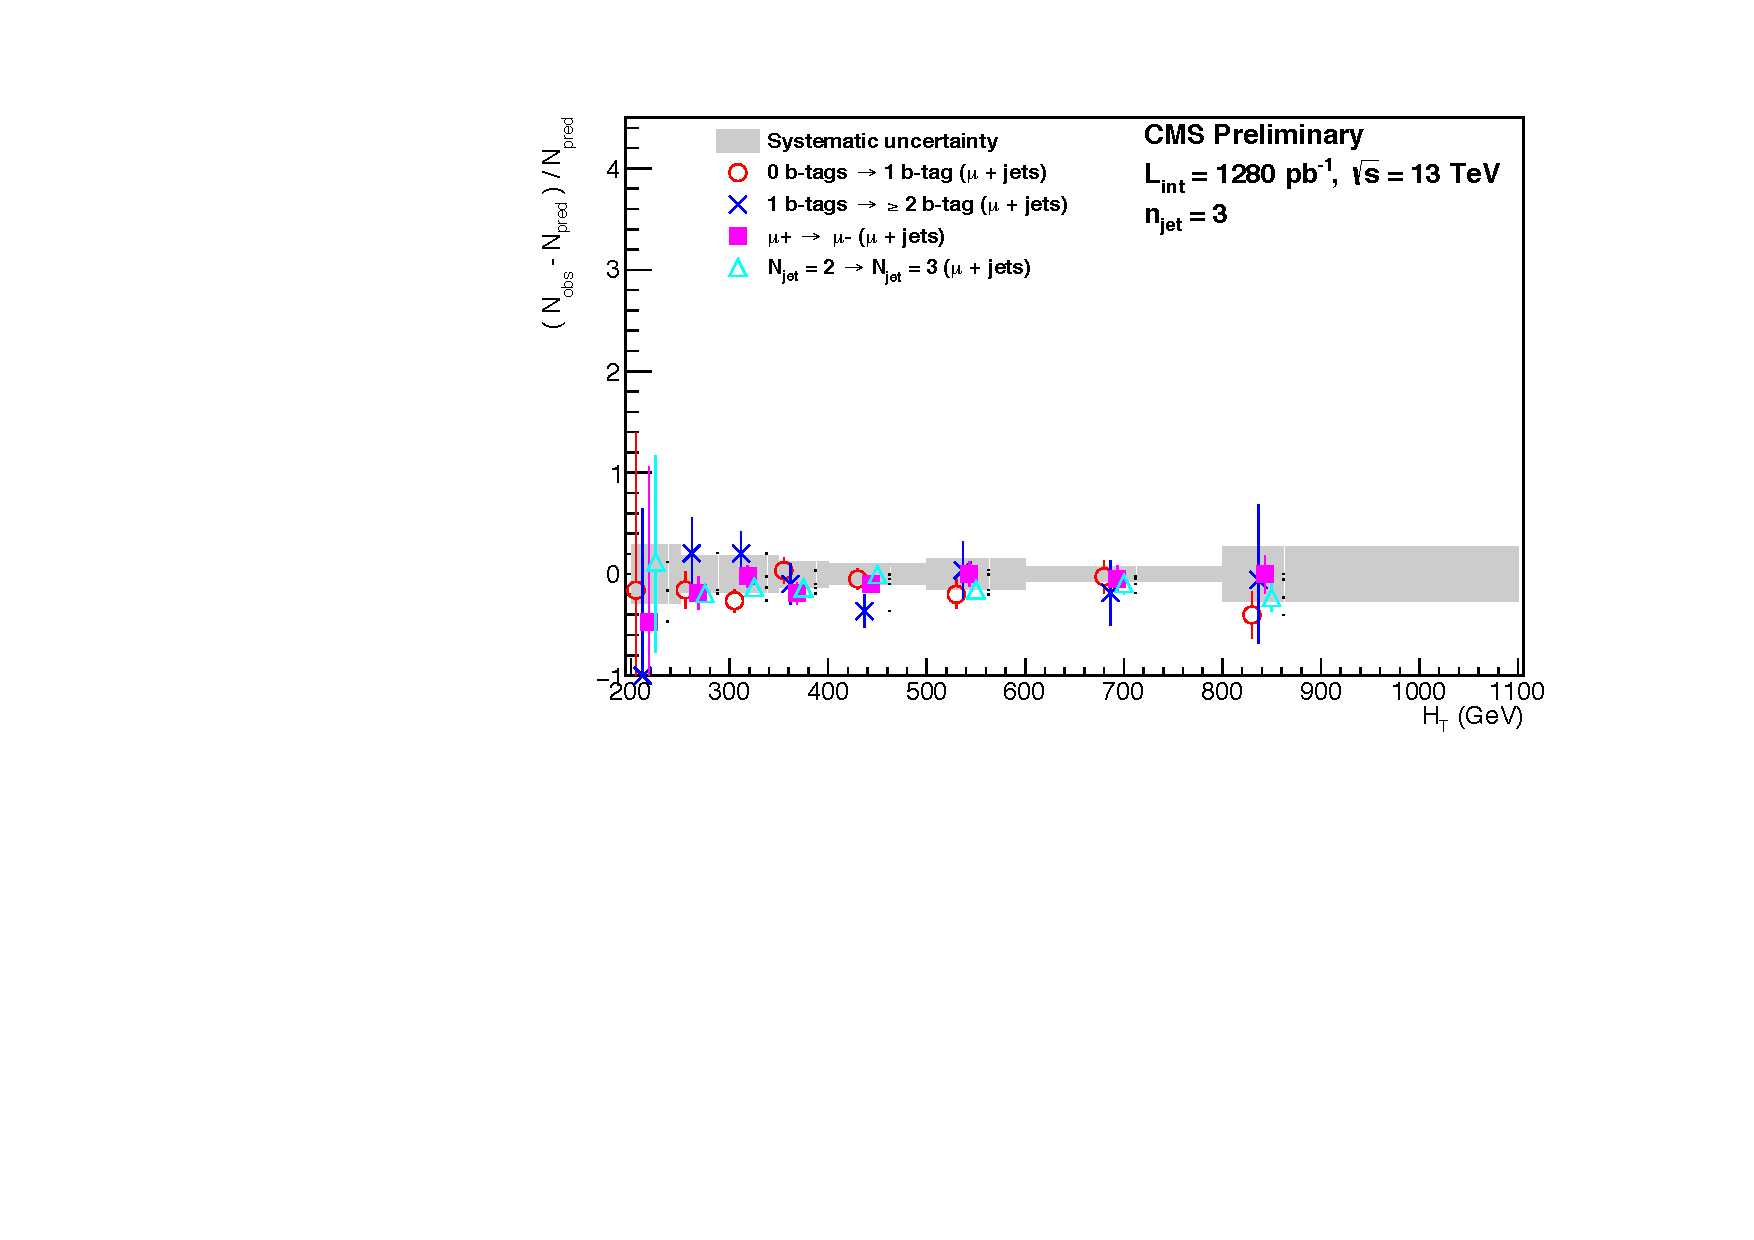
\includegraphics[width=0.5\textwidth]{figures/closureTests/1280pb/ttW/eq3j.pdf}} \\
%     \subfigure[$\njet =
%     4$]{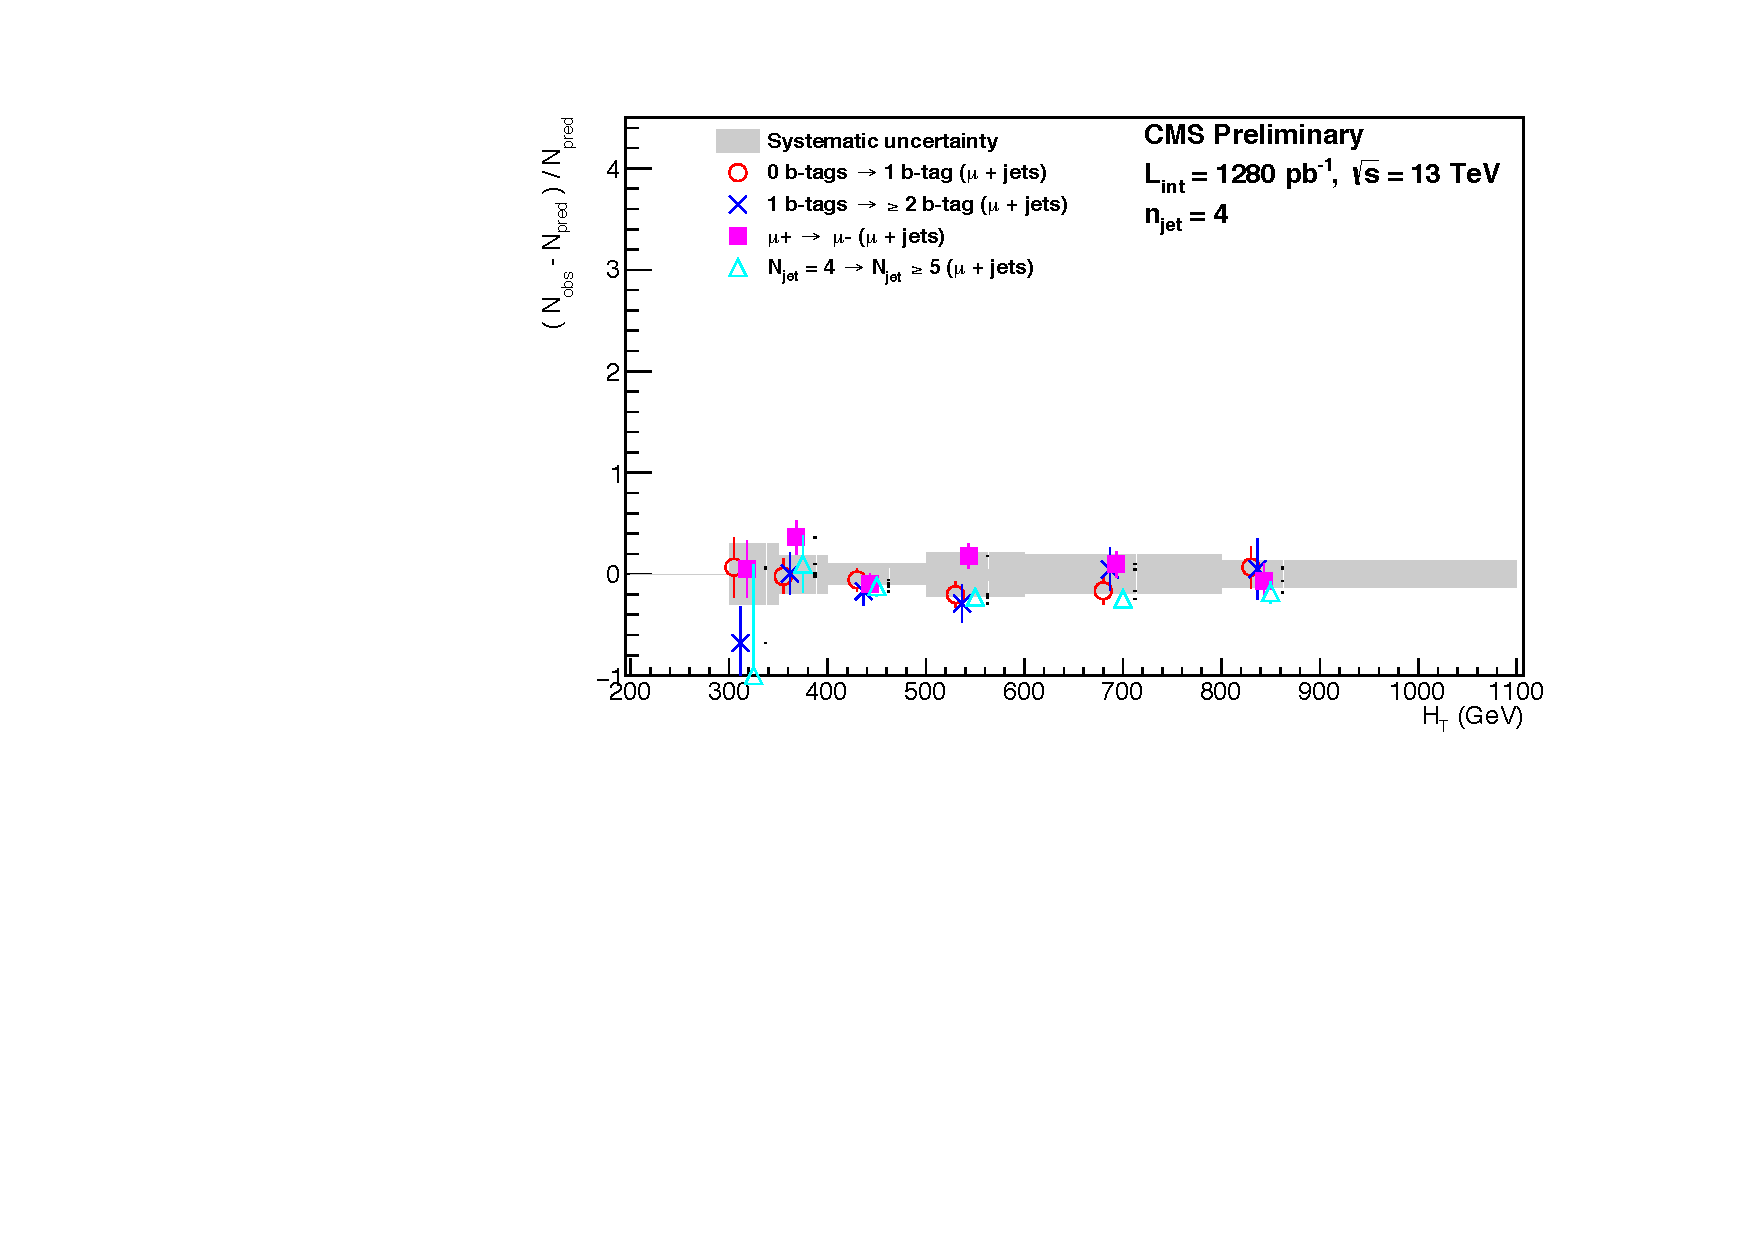
\includegraphics[width=0.5\textwidth]{figures/closureTests/1280pb/ttW/eq4j.pdf}} ~~
%     \subfigure[$\njet \geq
%     5$]{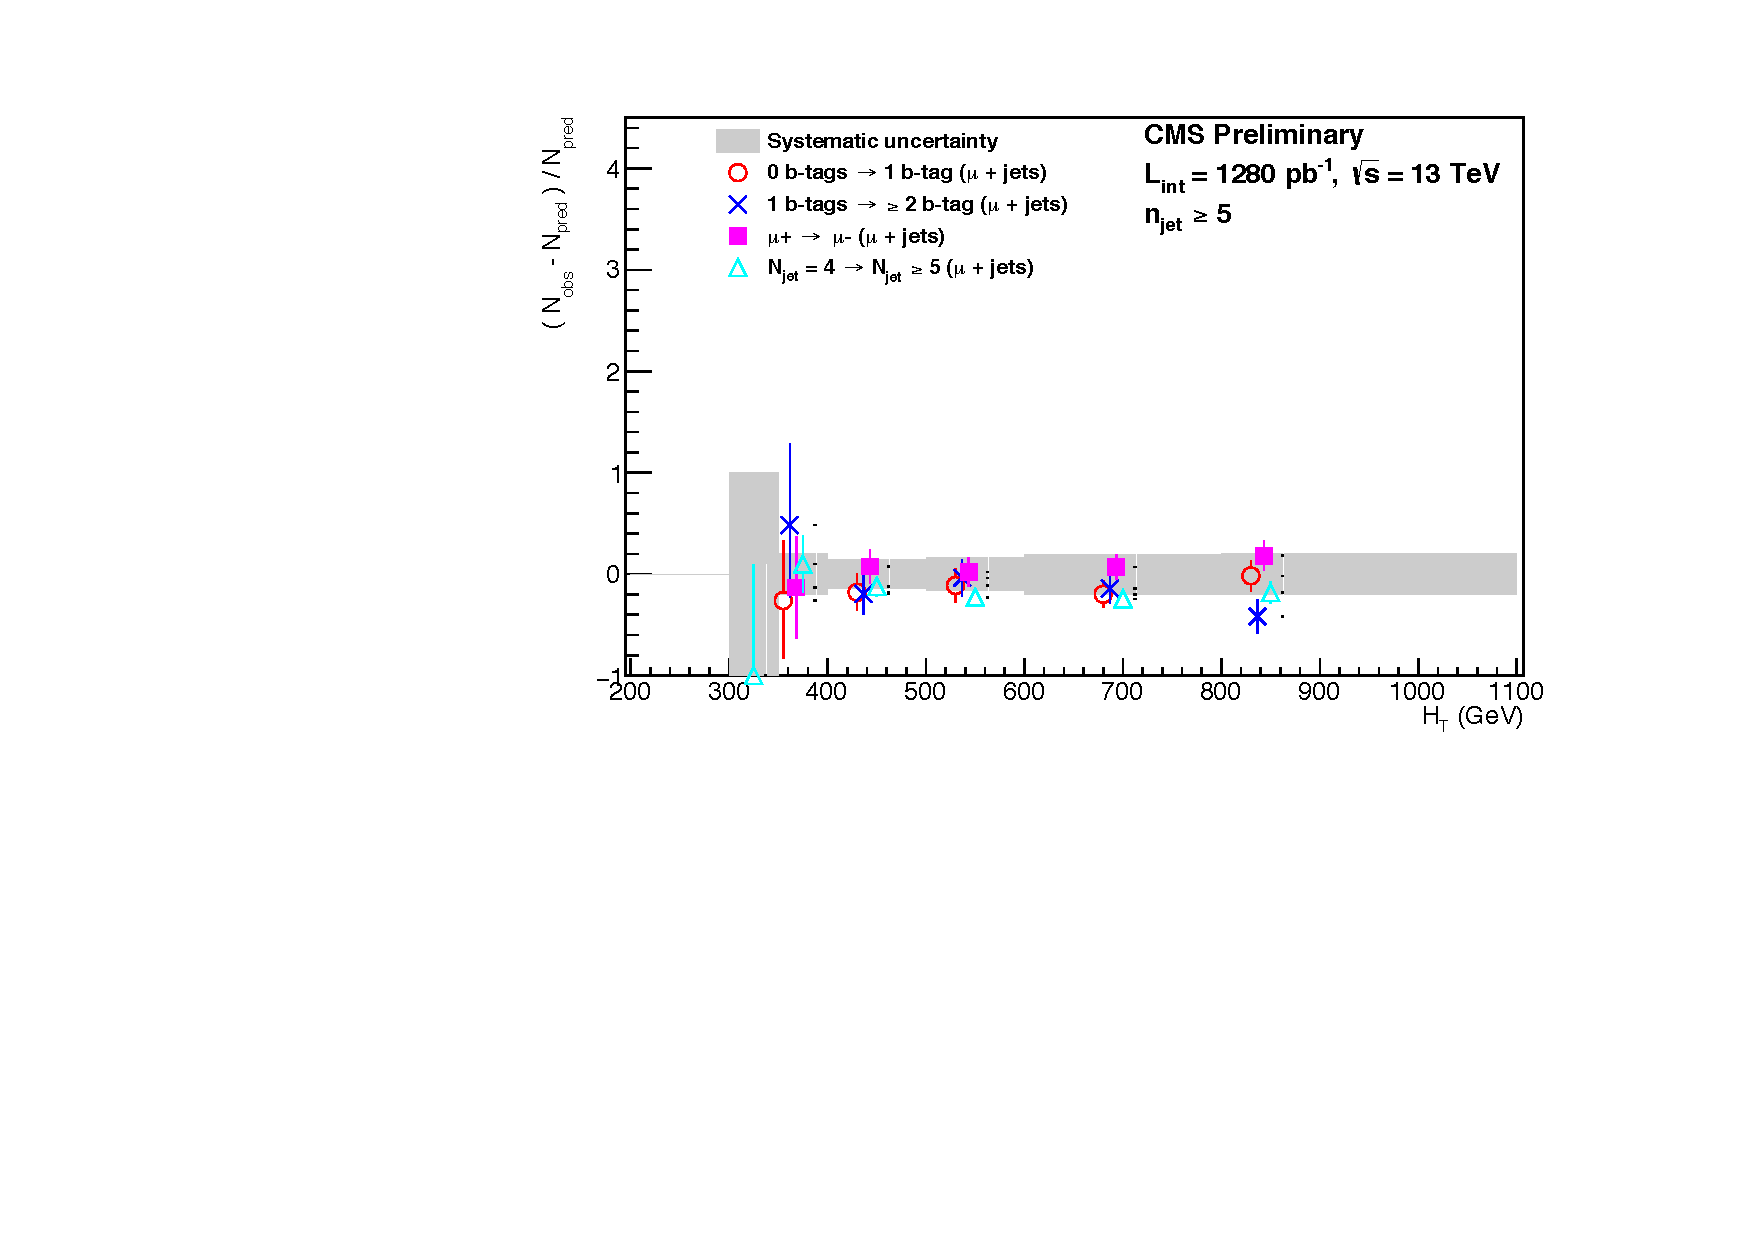
\includegraphics[width=0.5\textwidth]{figures/closureTests/1280pb/ttW/ge5j.pdf}} \\
%     \caption{Sets of closure tests (open symbols) designed to probe
%       the W and \ttbar + jets background, overlaid on top of
%       the systematic uncertainty estimates used for each of the seven
%       \scalht bins (shaded bands) carried out with $1.28\ifb$ of
%       $13\tev$ data. All events fit into the ``symmetric'' jet
%       category}
%     \label{fig:ttWclosureDataSym}
%   \end{center} 
% \end{figure}
%
% \begin{figure}[h!]
%   \begin{center}
%     \subfigure[$\njet =
%     2$]{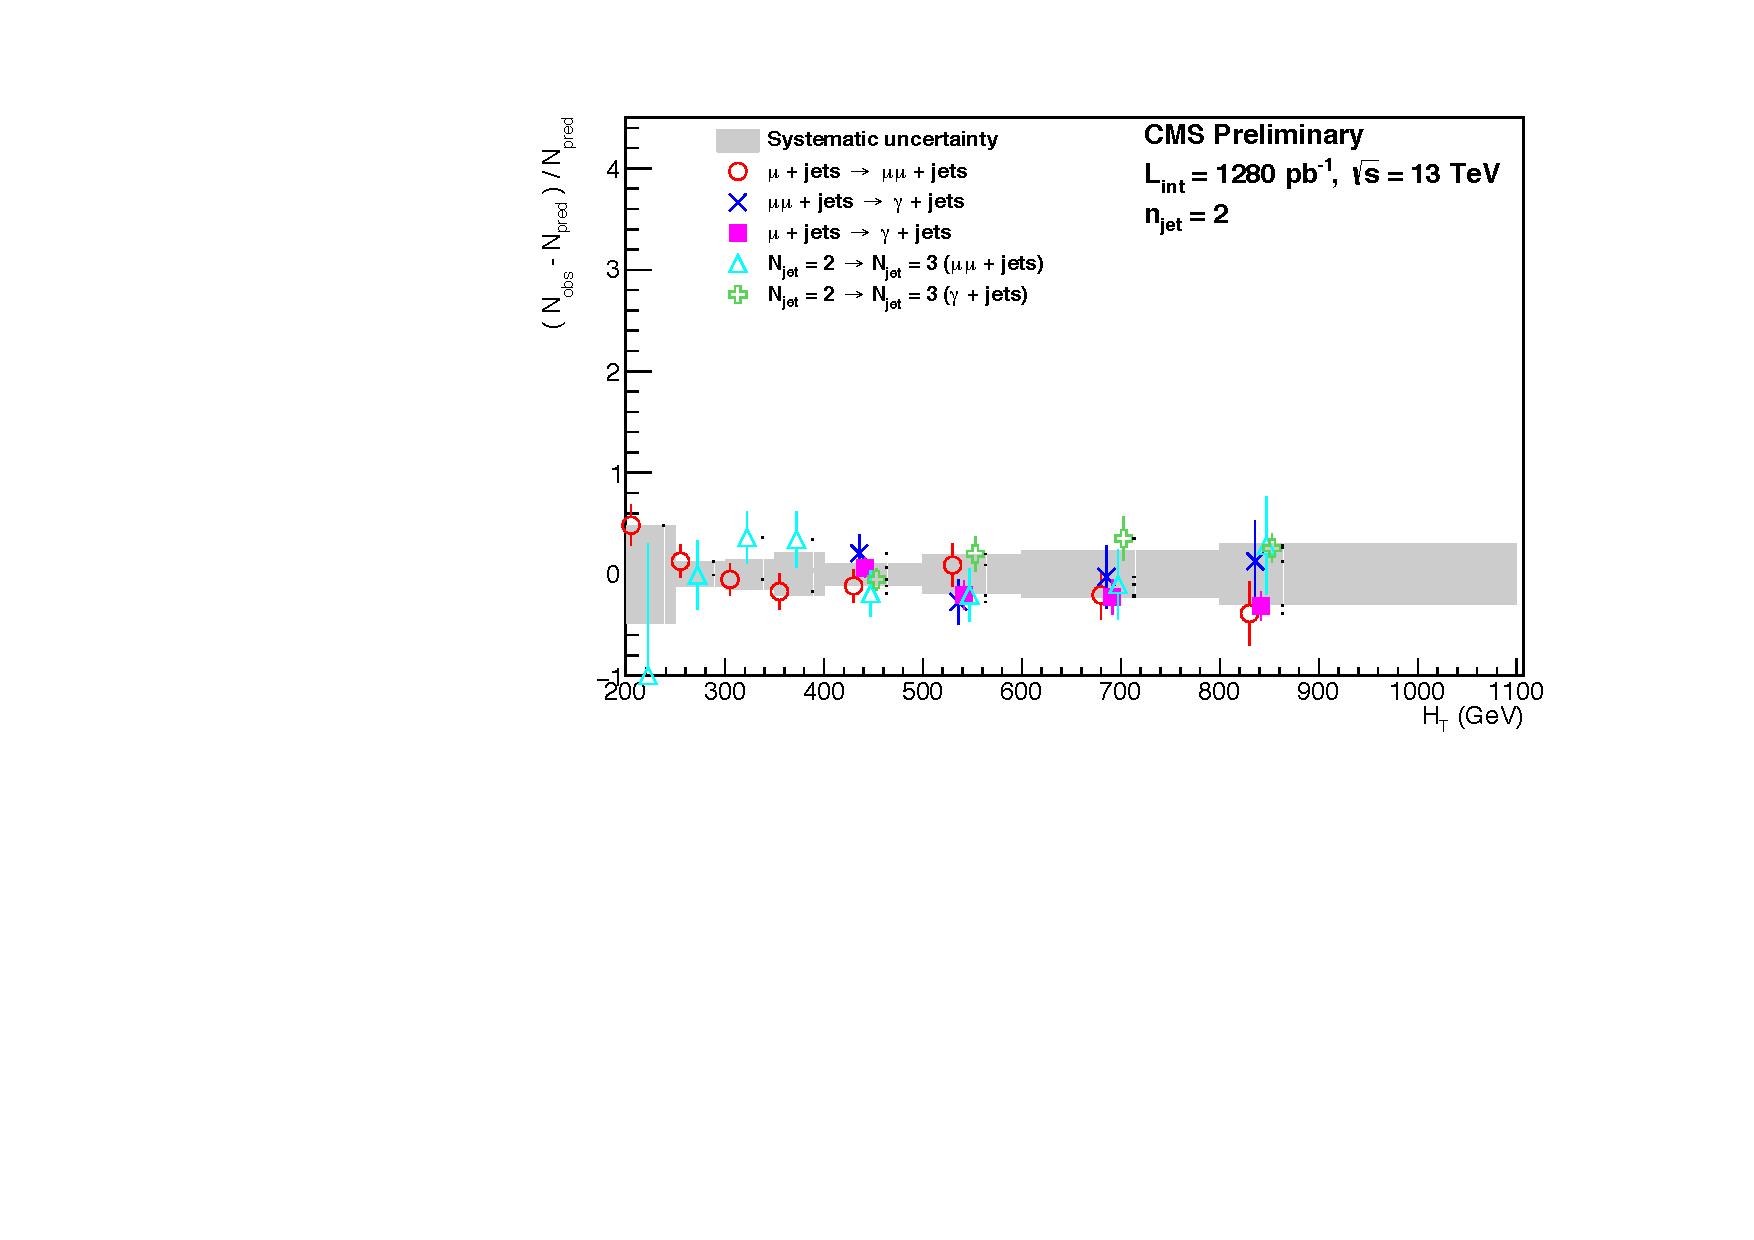
\includegraphics[width=0.5\textwidth]{figures/closureTests/1280pb/Zinv/eq2j.pdf}} ~~
%     \subfigure[$\njet =
%     3$]{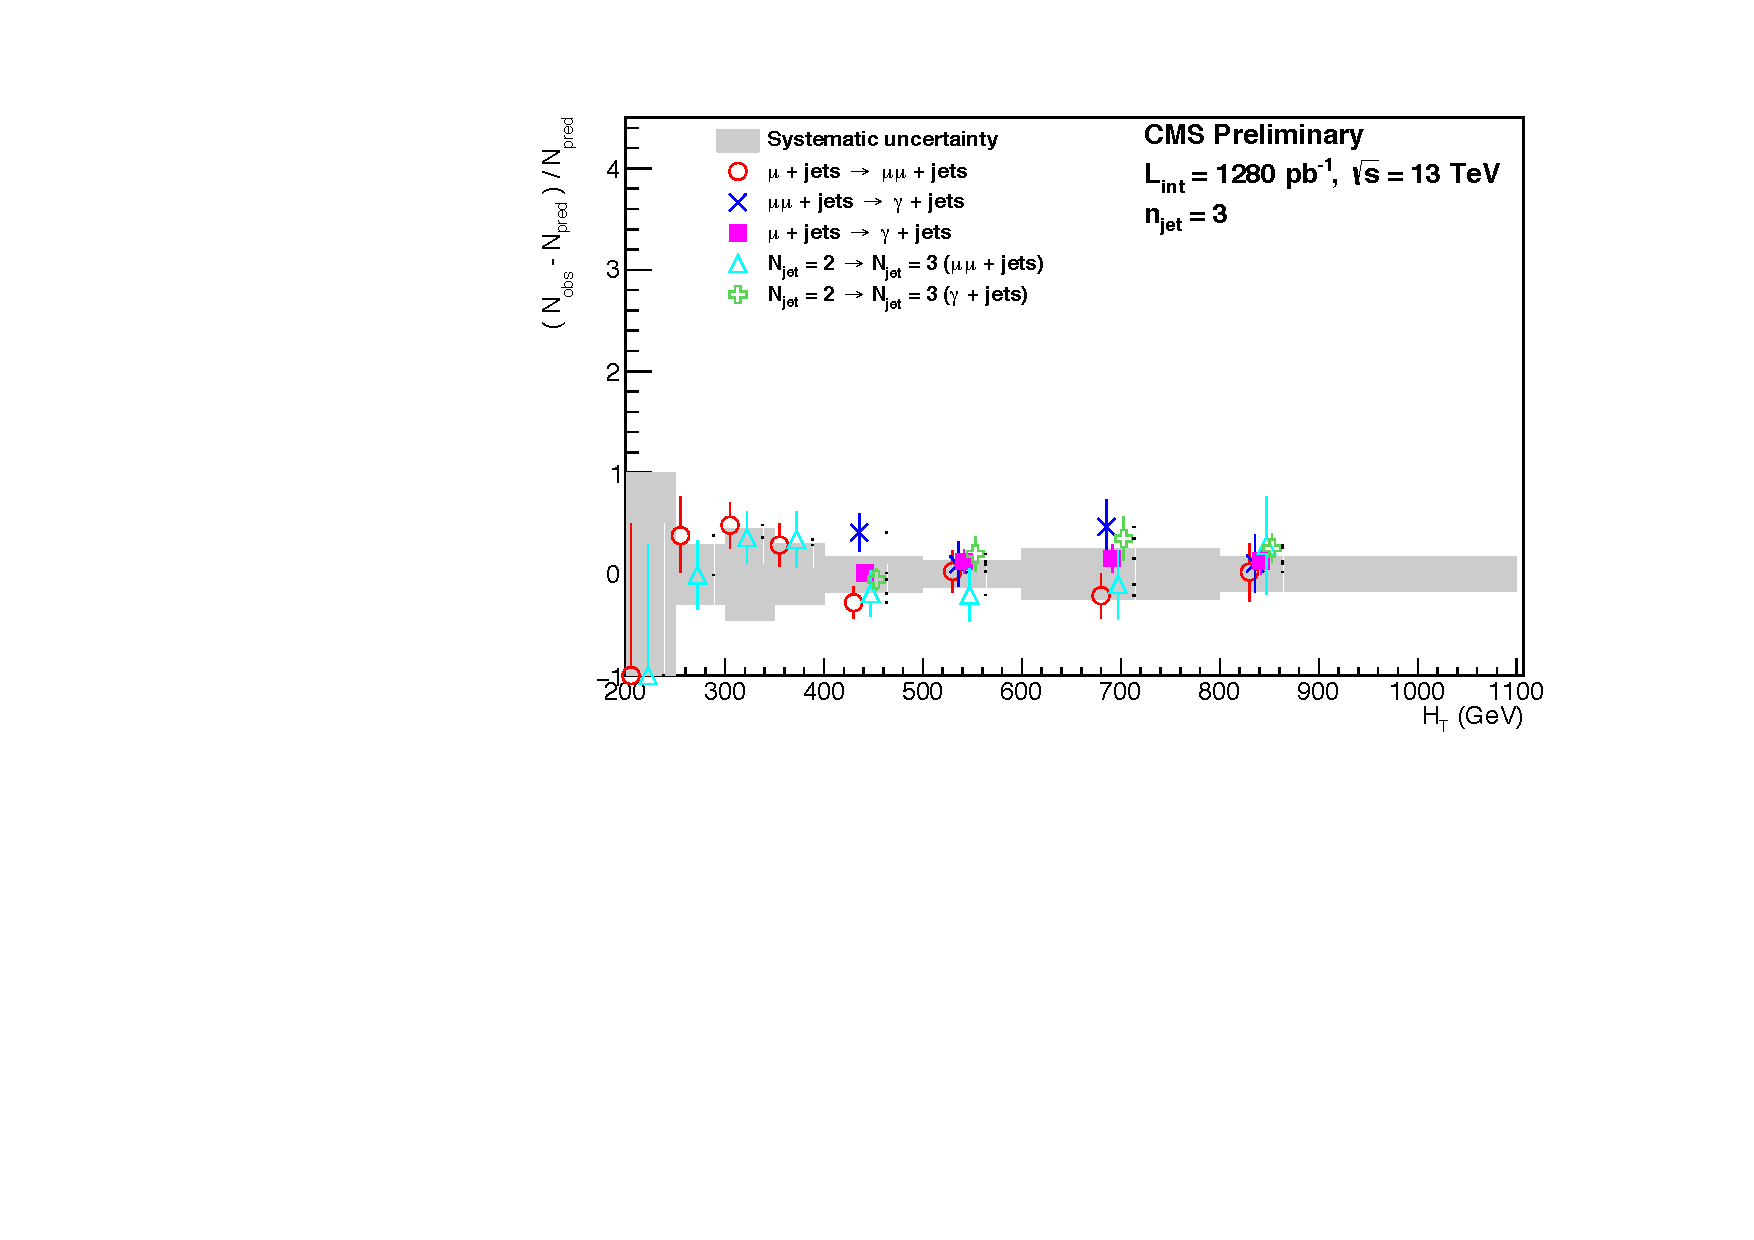
\includegraphics[width=0.5\textwidth]{figures/closureTests/1280pb/Zinv/eq3j.pdf}} \\
%     \subfigure[$\njet =
%     4$]{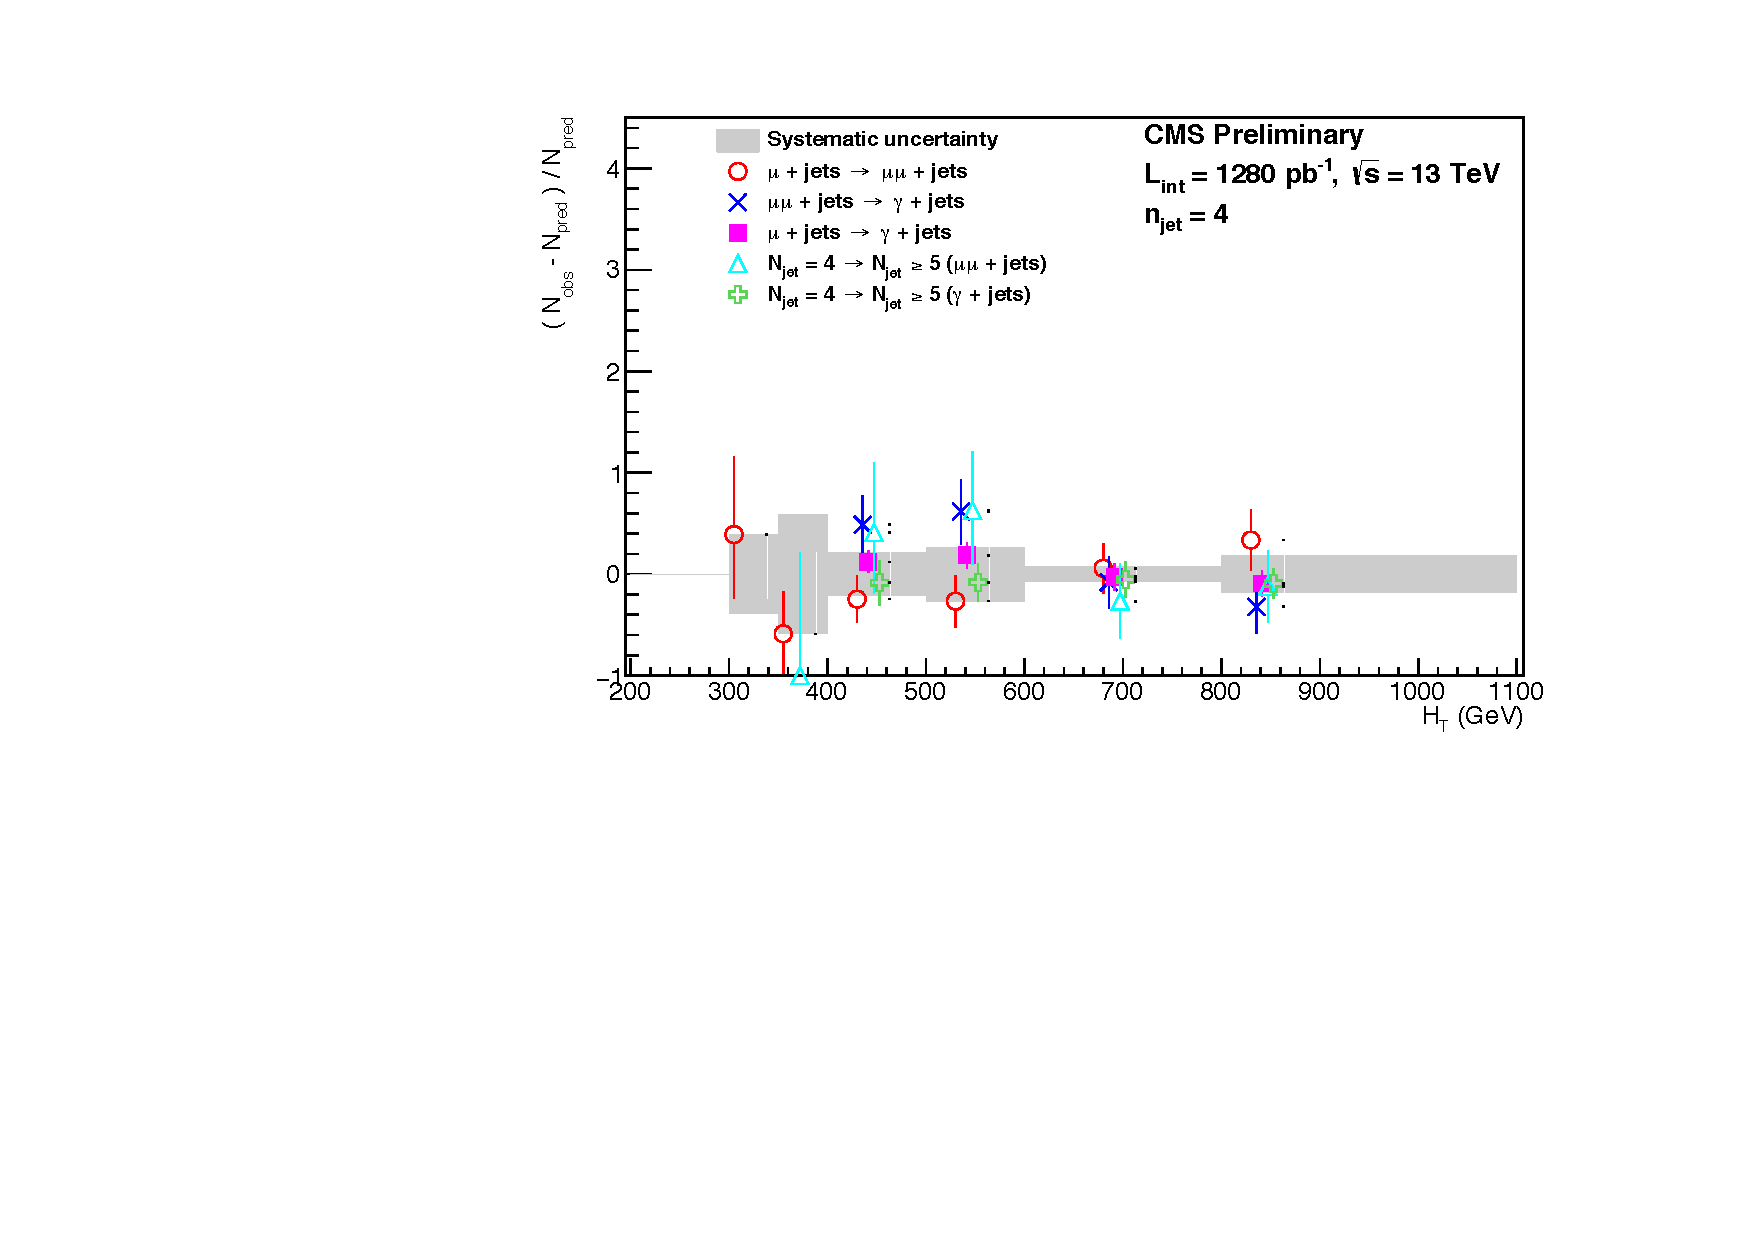
\includegraphics[width=0.5\textwidth]{figures/closureTests/1280pb/Zinv/eq4j.pdf}} ~~
%     \subfigure[$\njet \geq
%     5$]{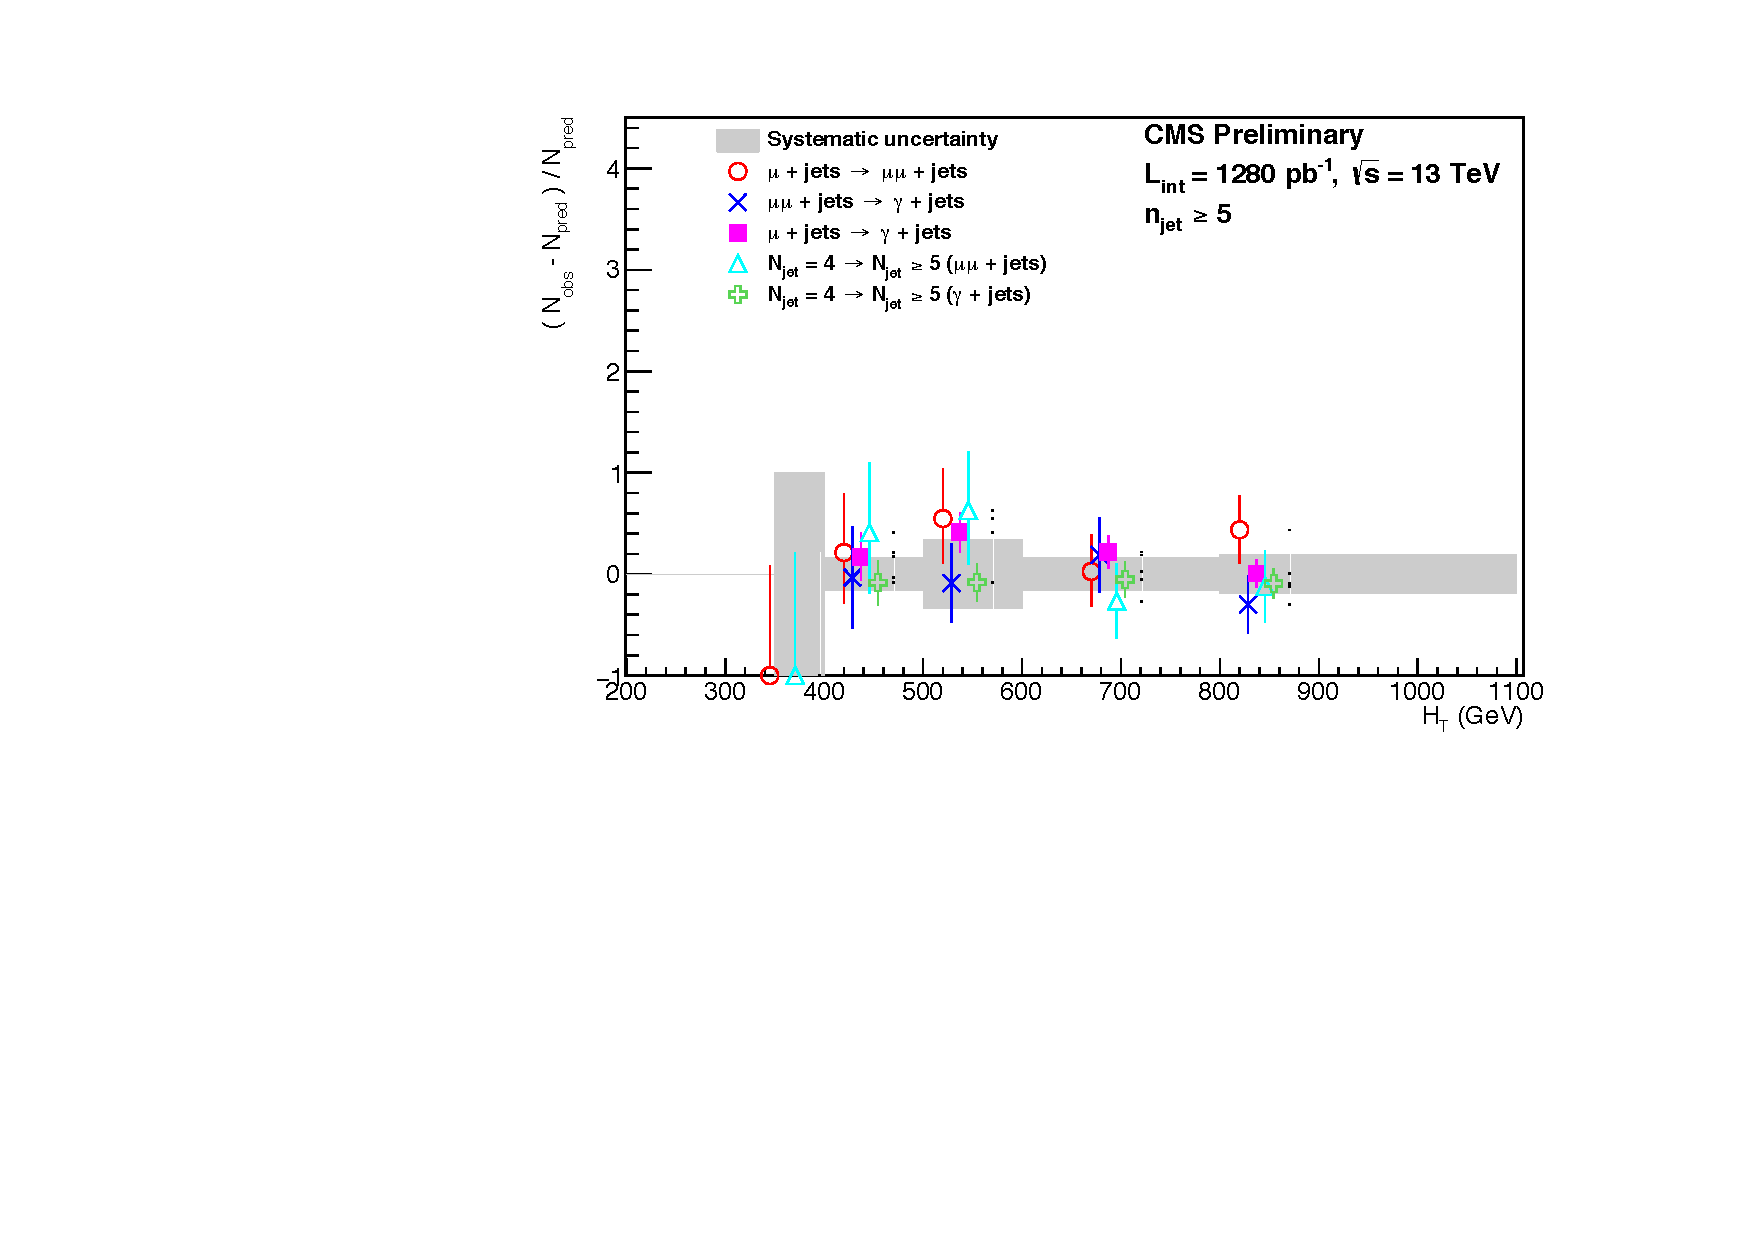
\includegraphics[width=0.5\textwidth]{figures/closureTests/1280pb/Zinv/ge5j.pdf}} \\
%     \caption{Sets of closure tests (open symbols) designed to probe
%       the \znunu + jets background, overlaid on top of
%       the systematic uncertainty estimates used for each of the seven
%       \scalht bins (shaded bands) carried out with $1.28\ifb$ of
%       $13\tev$ data. All events fit into the ``symmetric'' jet
%       category}
%     \label{fig:ZinvclosureDataSym}
%   \end{center} 
% \end{figure}
%
% \begin{figure}[h!]
%   \begin{center}
%     \subfigure[$\njet =
%     2$]{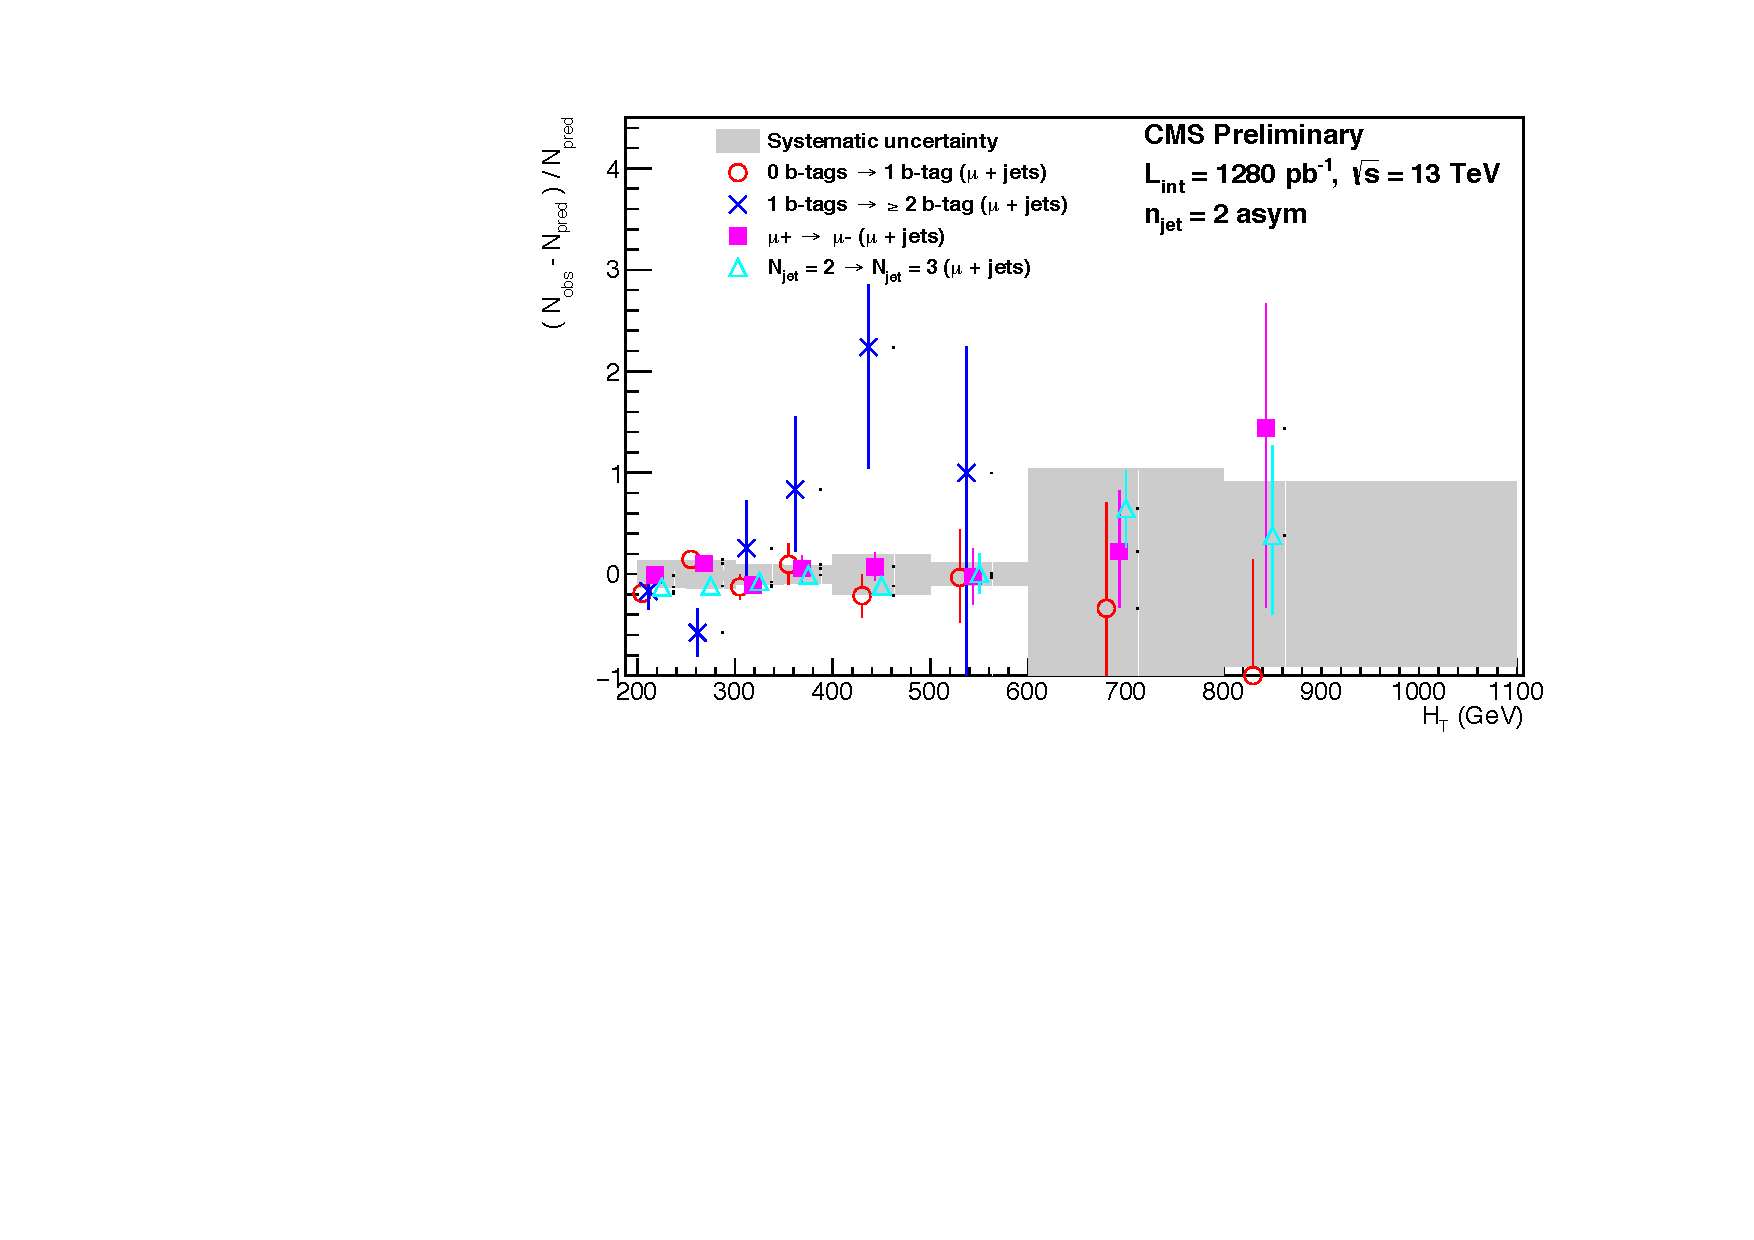
\includegraphics[width=0.5\textwidth]{figures/closureTests/1280pb/ttW/eq2a.pdf}} ~~
%     \subfigure[$\njet =
%     3$]{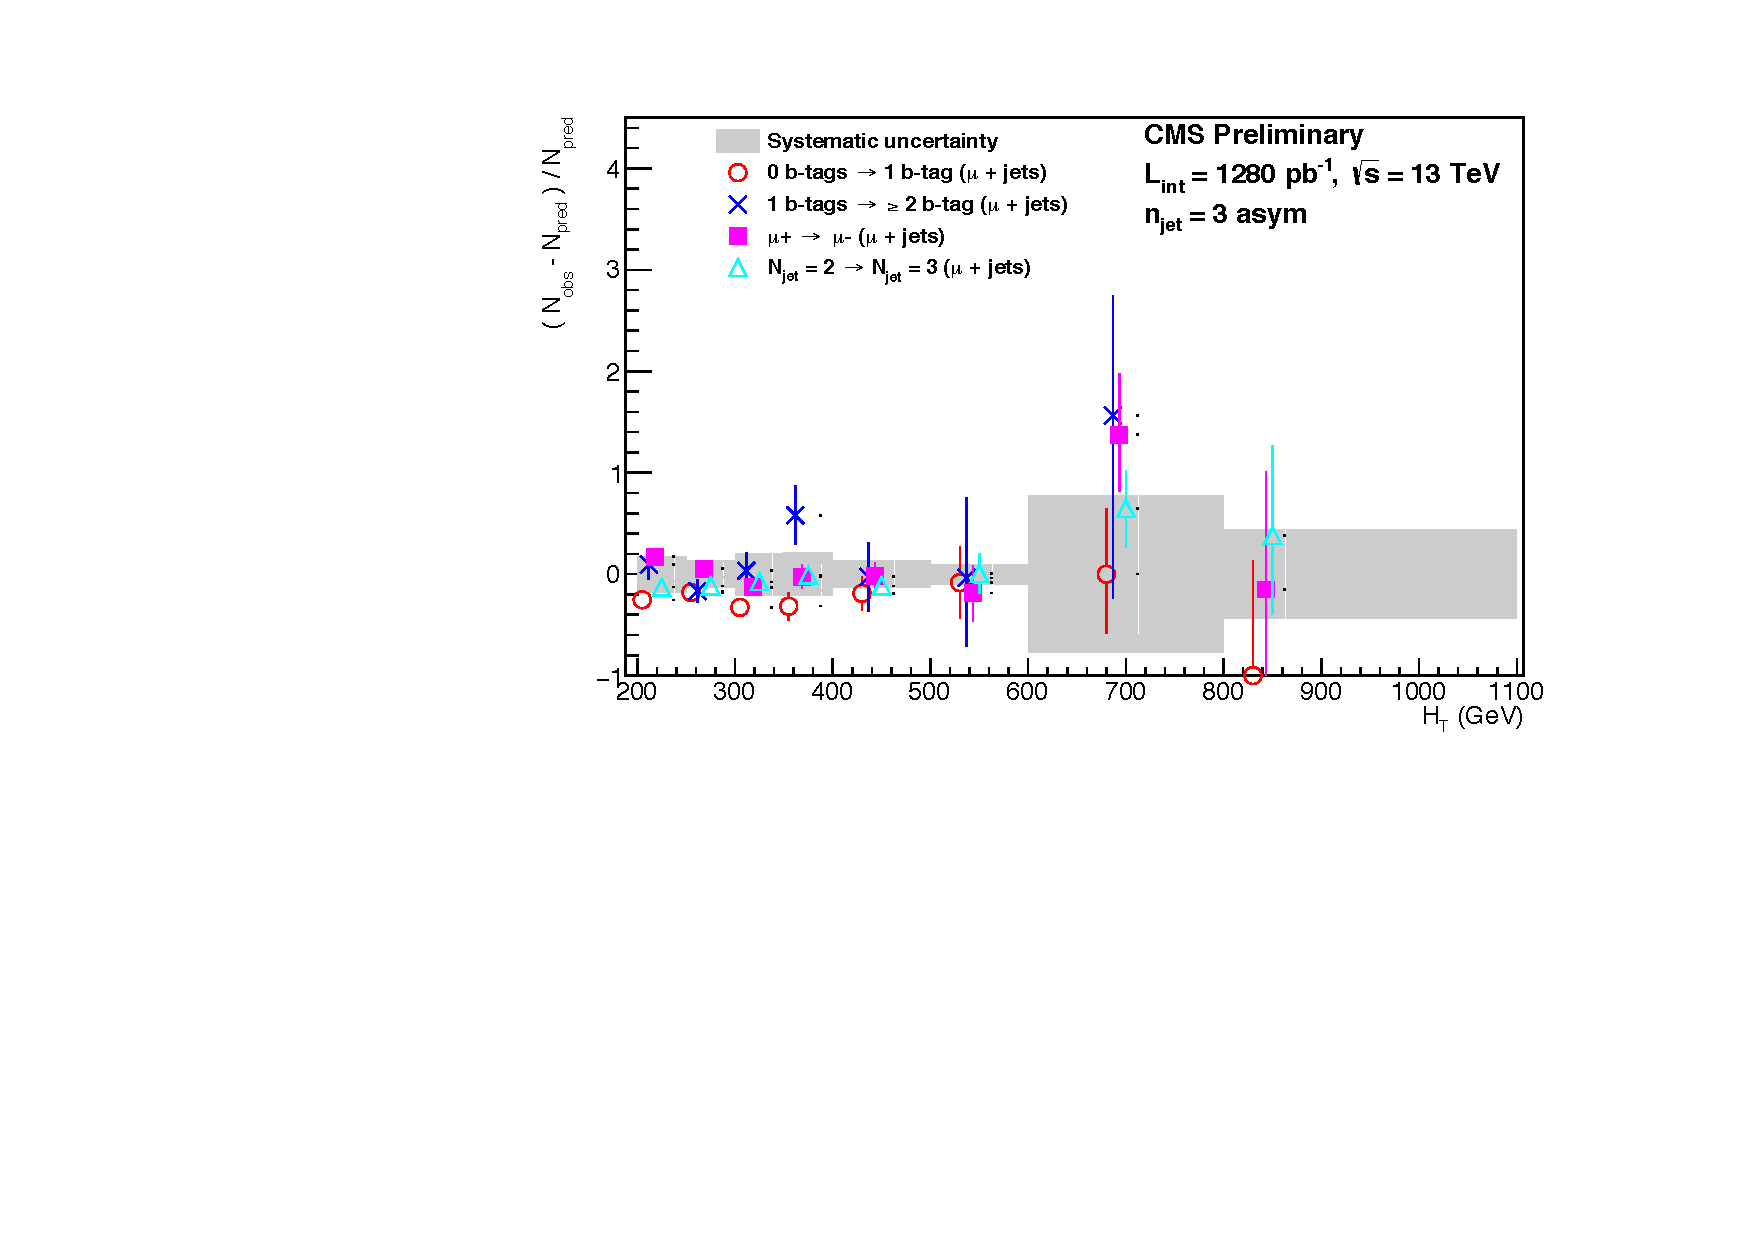
\includegraphics[width=0.5\textwidth]{figures/closureTests/1280pb/ttW/eq3a.pdf}} \\
%     \subfigure[$\njet =
%     4$]{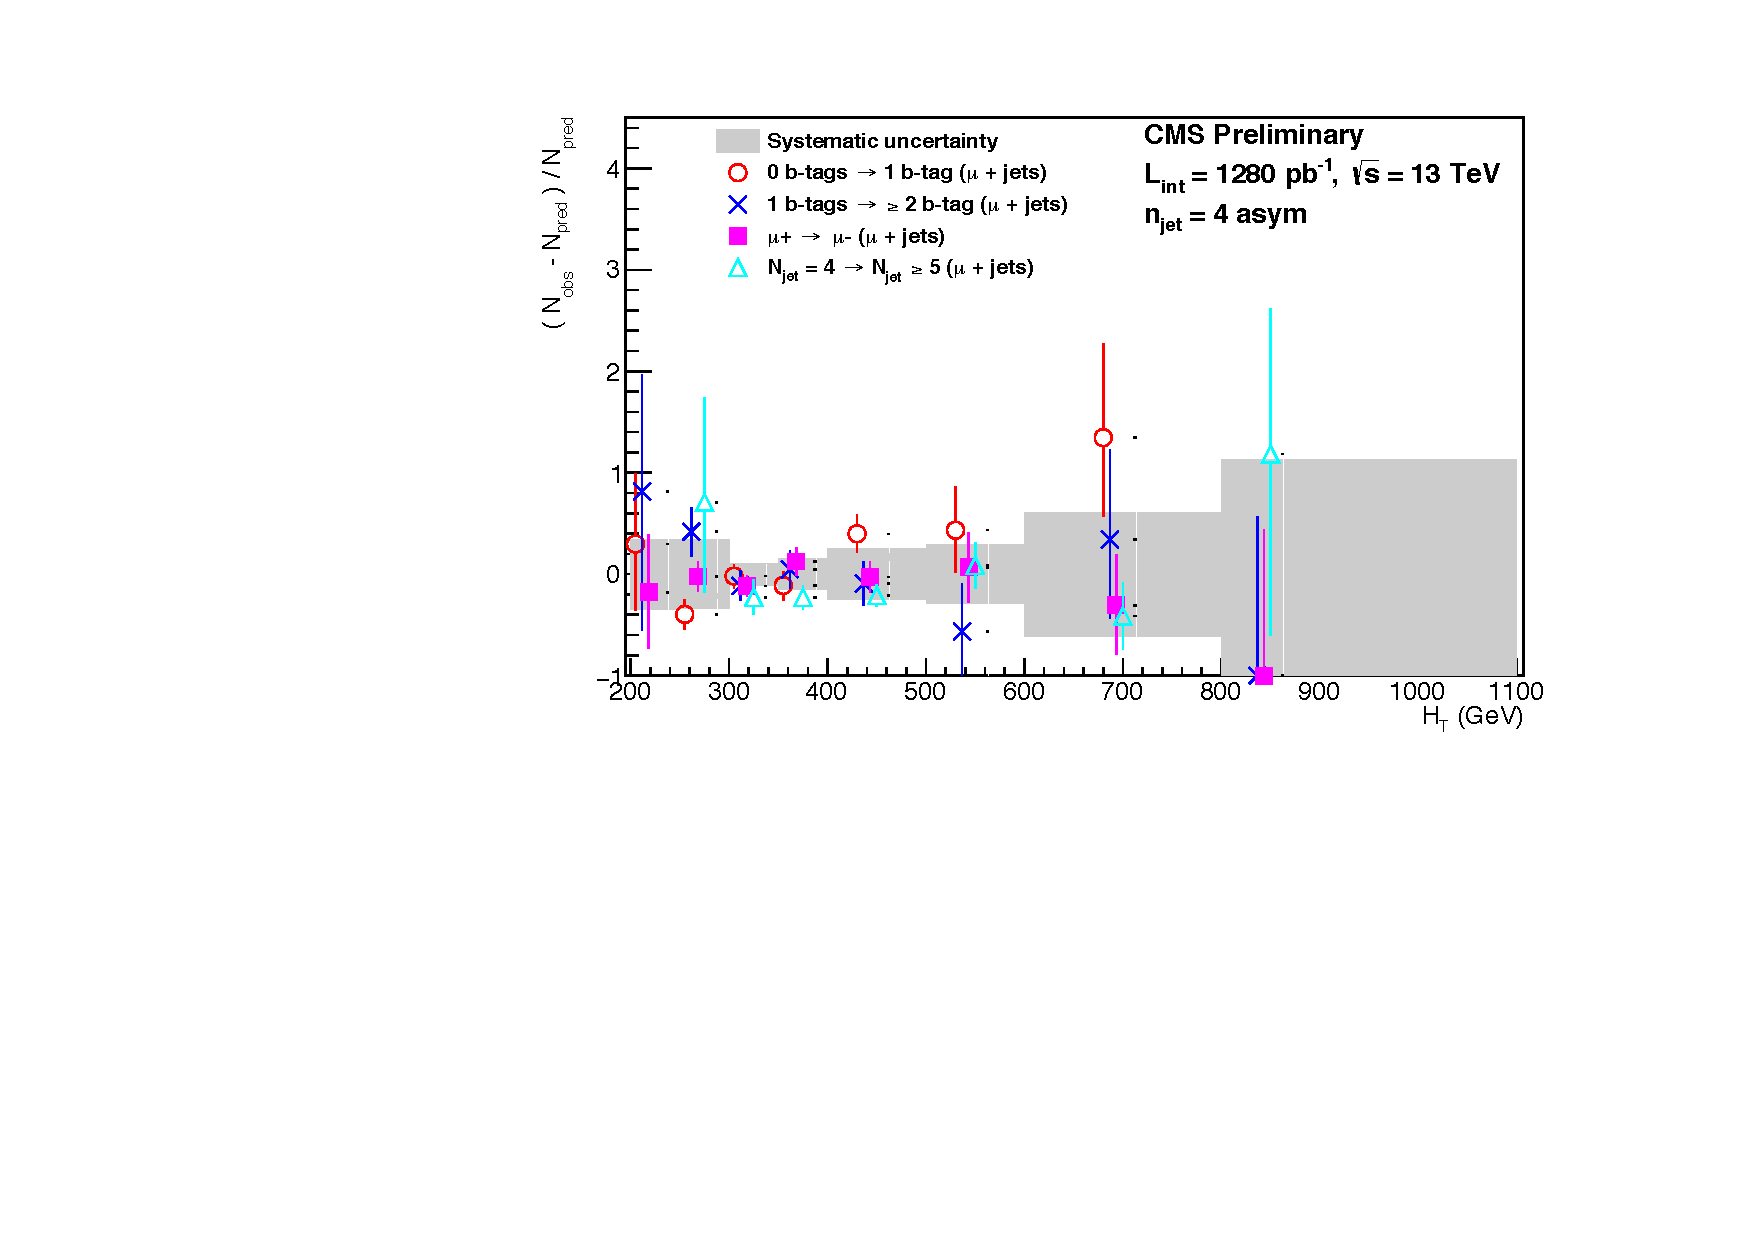
\includegraphics[width=0.5\textwidth]{figures/closureTests/1280pb/ttW/eq4a.pdf}} ~~
%     \subfigure[$\njet \geq
%     5$]{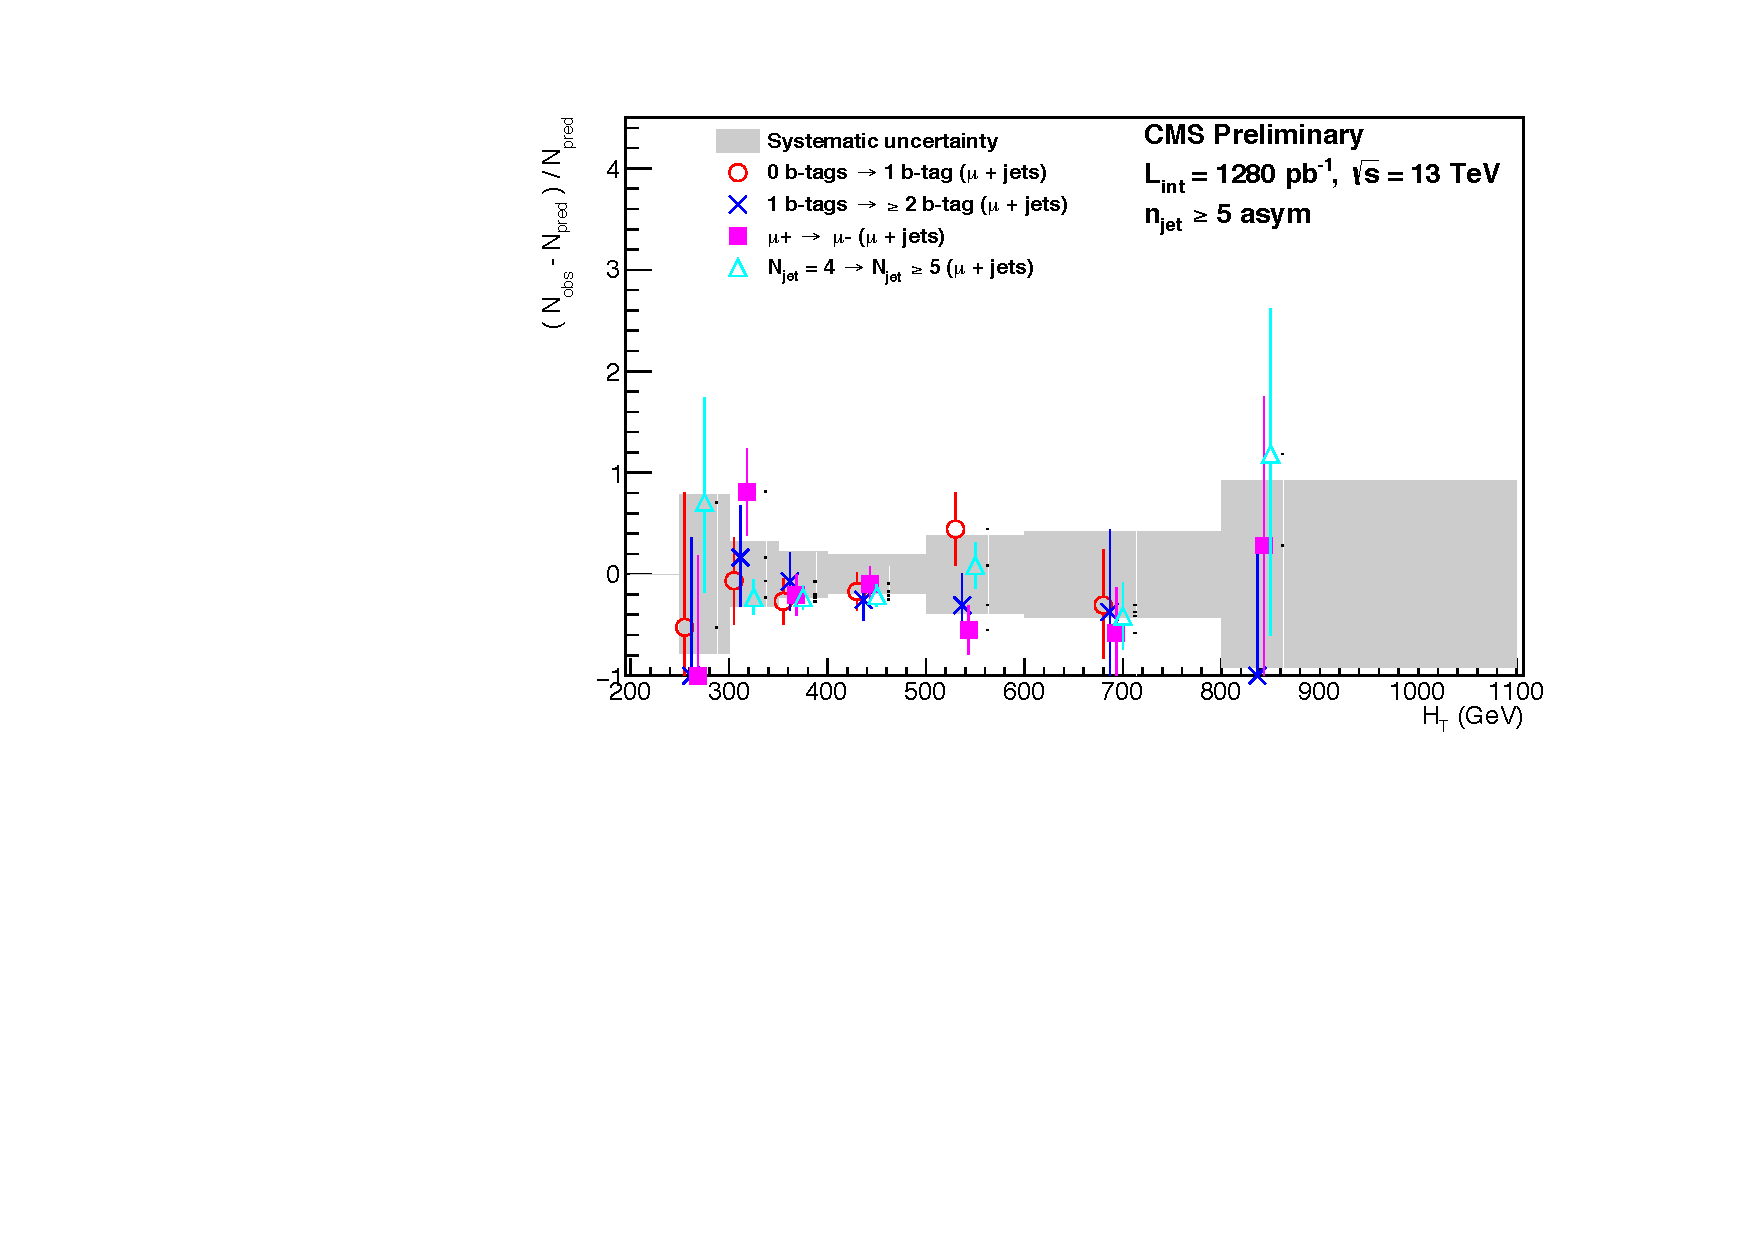
\includegraphics[width=0.5\textwidth]{figures/closureTests/1280pb/ttW/ge5a.pdf}} \\
%     \caption{Sets of closure tests (open symbols) designed to probe
%       the W and \ttbar + jets overlaid on top of
%       the systematic uncertainty estimates used for each of the seven
%       \scalht bins (shaded bands) carried out with $1.28\ifb$ of
%       $13\tev$ data. All events fit into the ``asymmetric'' jet
%       category}
%     \label{fig:ttWclosureDataAsym}
%   \end{center} 
% \end{figure}
%
% \begin{figure}[h!]
%   \begin{center}
%     \subfigure[$\njet =
%     2$]{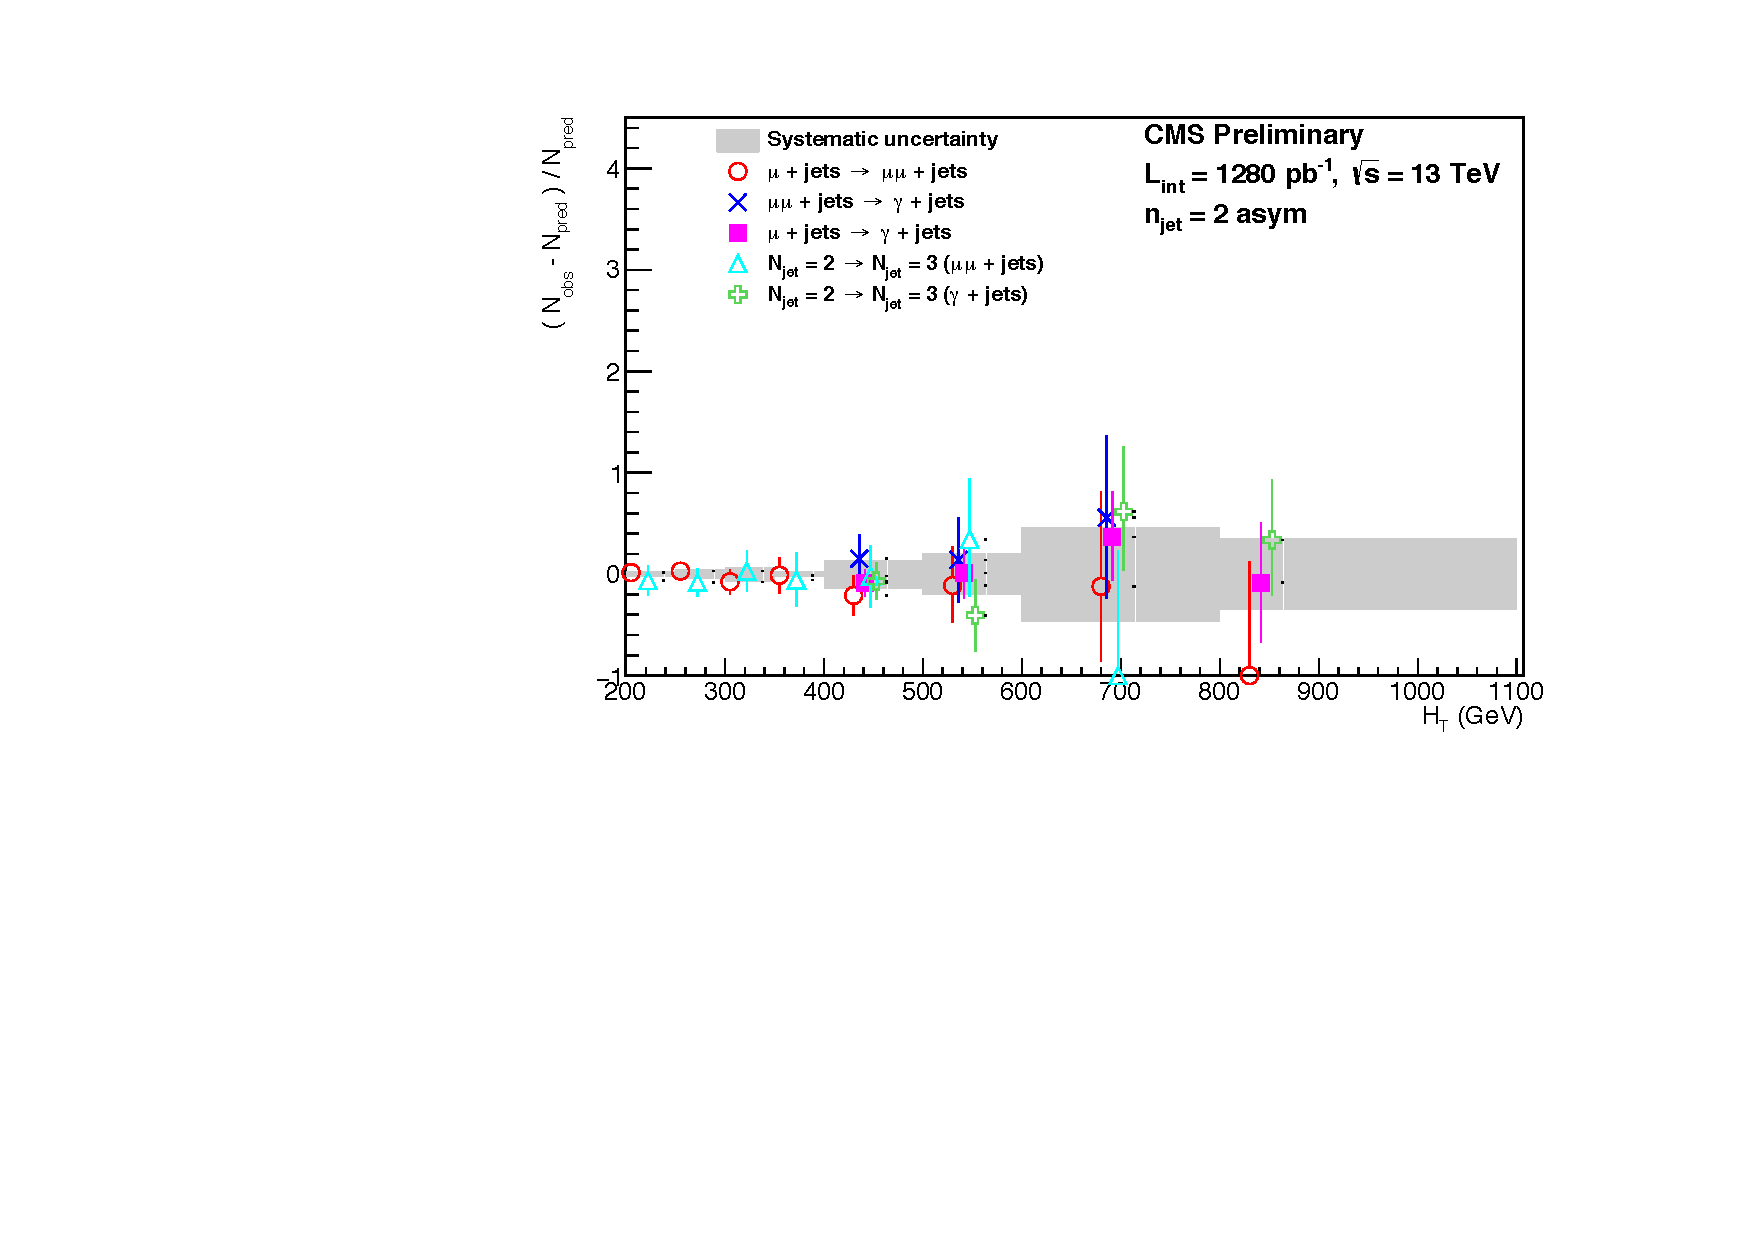
\includegraphics[width=0.5\textwidth]{figures/closureTests/1280pb/Zinv/eq2a.pdf}} ~~
%     \subfigure[$\njet =
%     3$]{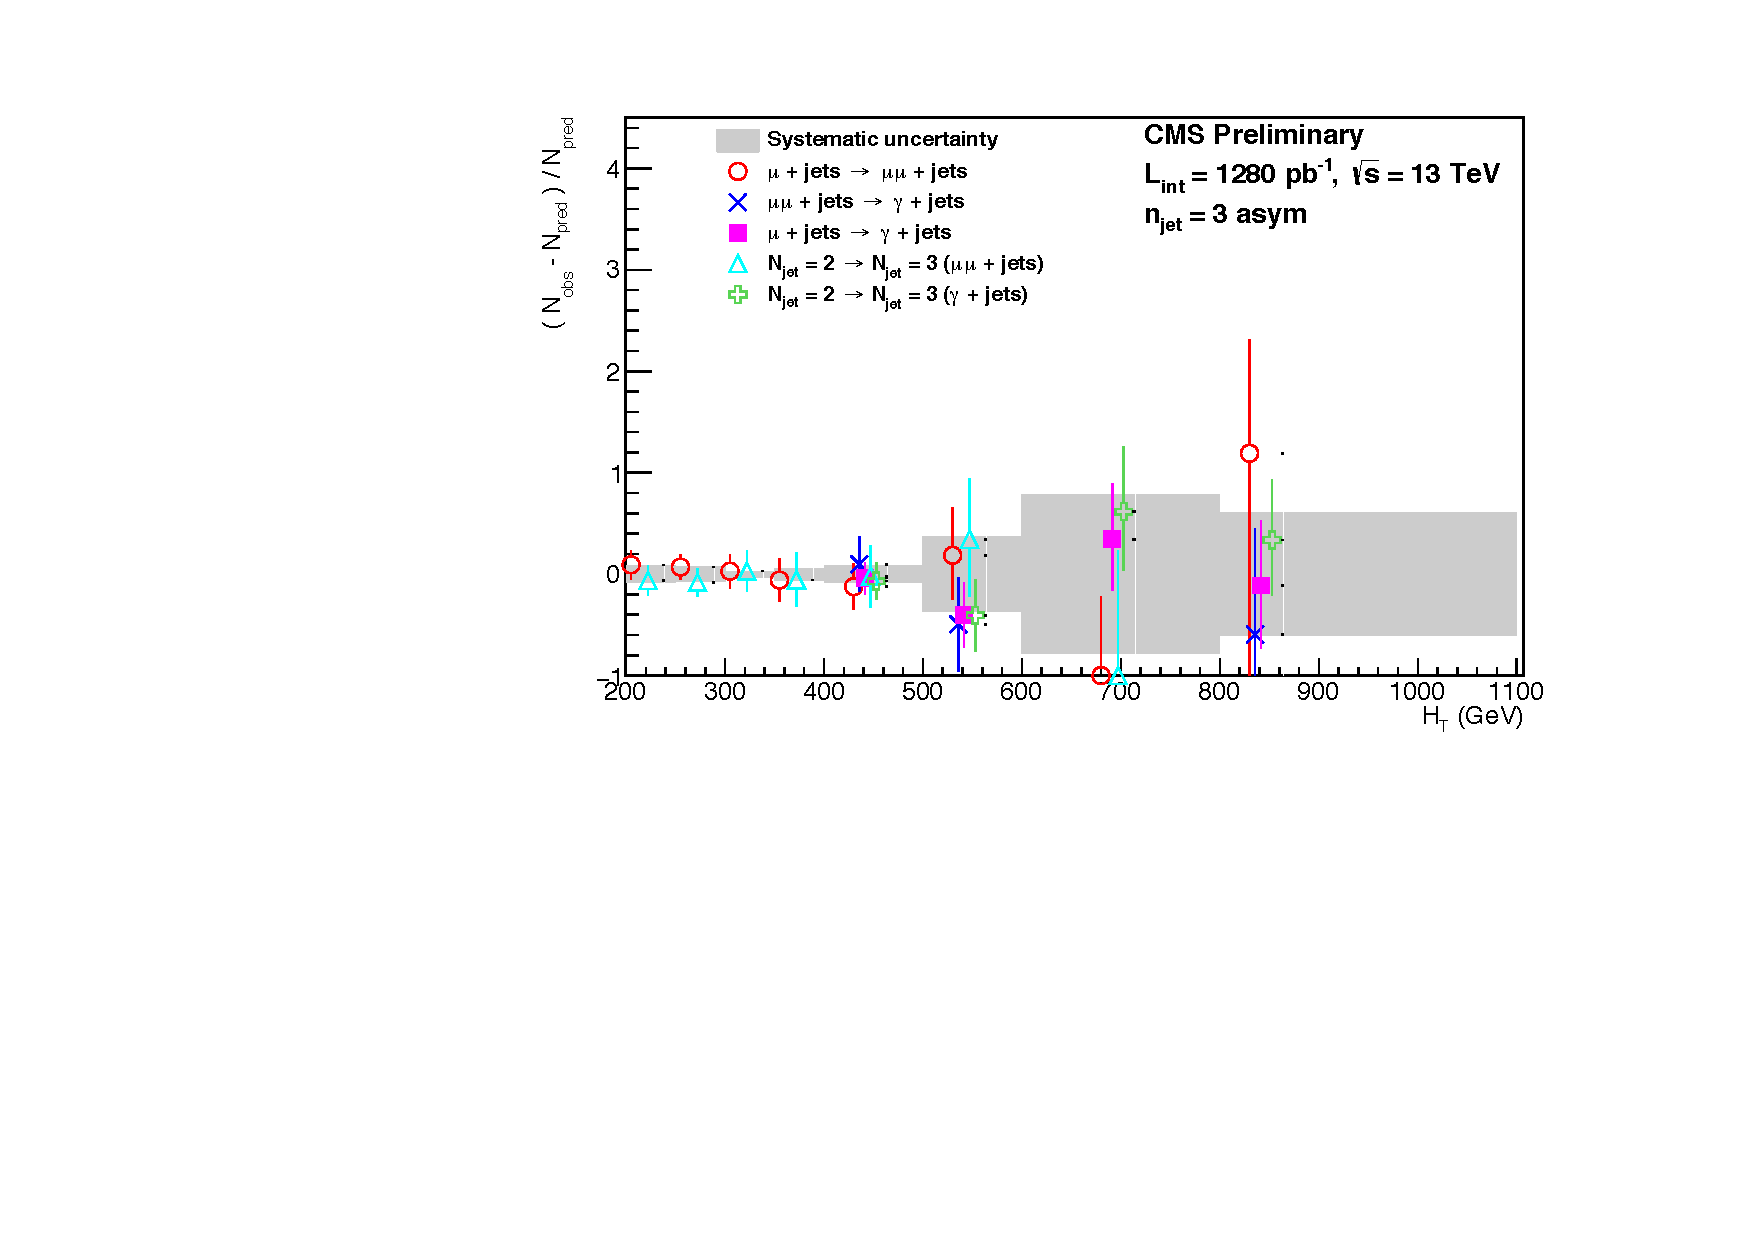
\includegraphics[width=0.5\textwidth]{figures/closureTests/1280pb/Zinv/eq3a.pdf}} \\
%     \subfigure[$\njet =
%     4$]{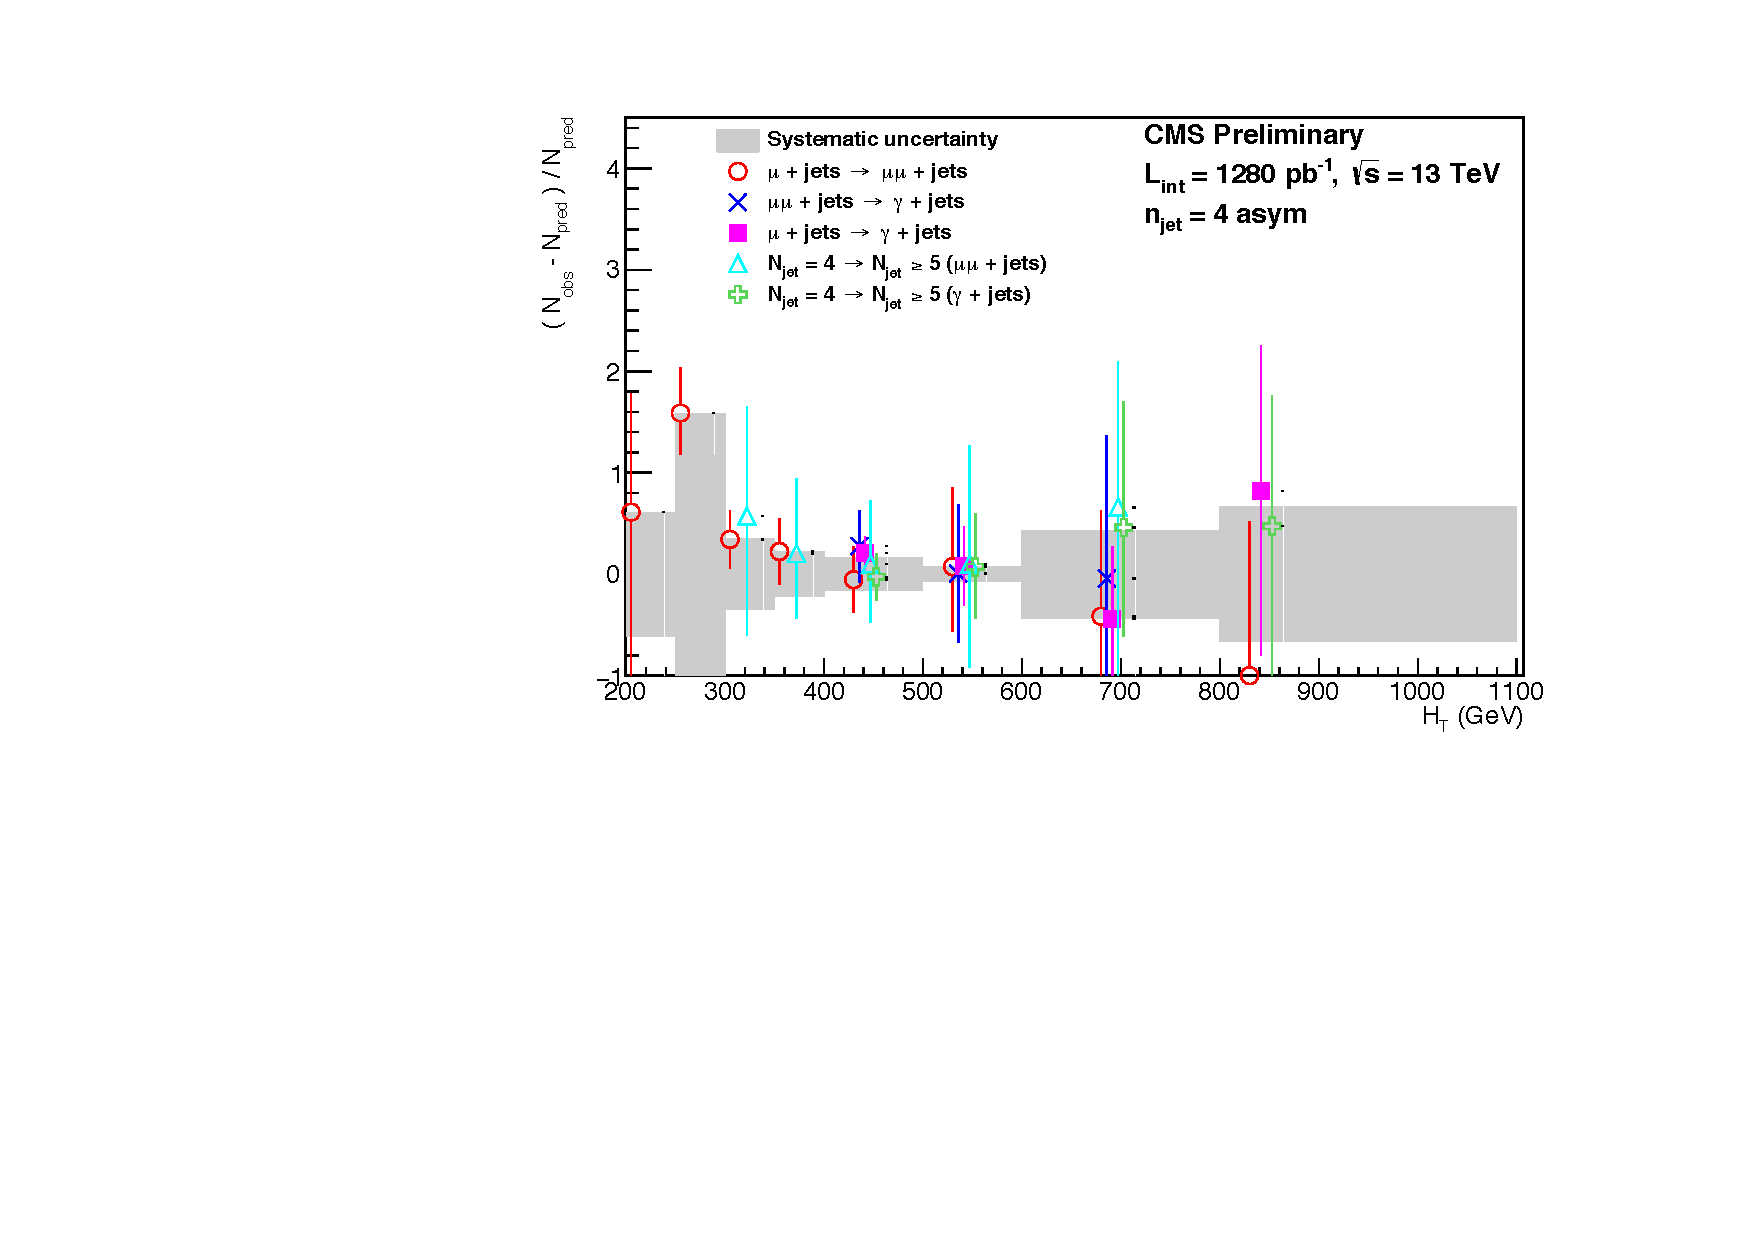
\includegraphics[width=0.5\textwidth]{figures/closureTests/1280pb/Zinv/eq4a.pdf}} ~~
%     \subfigure[$\njet \geq
%     5$]{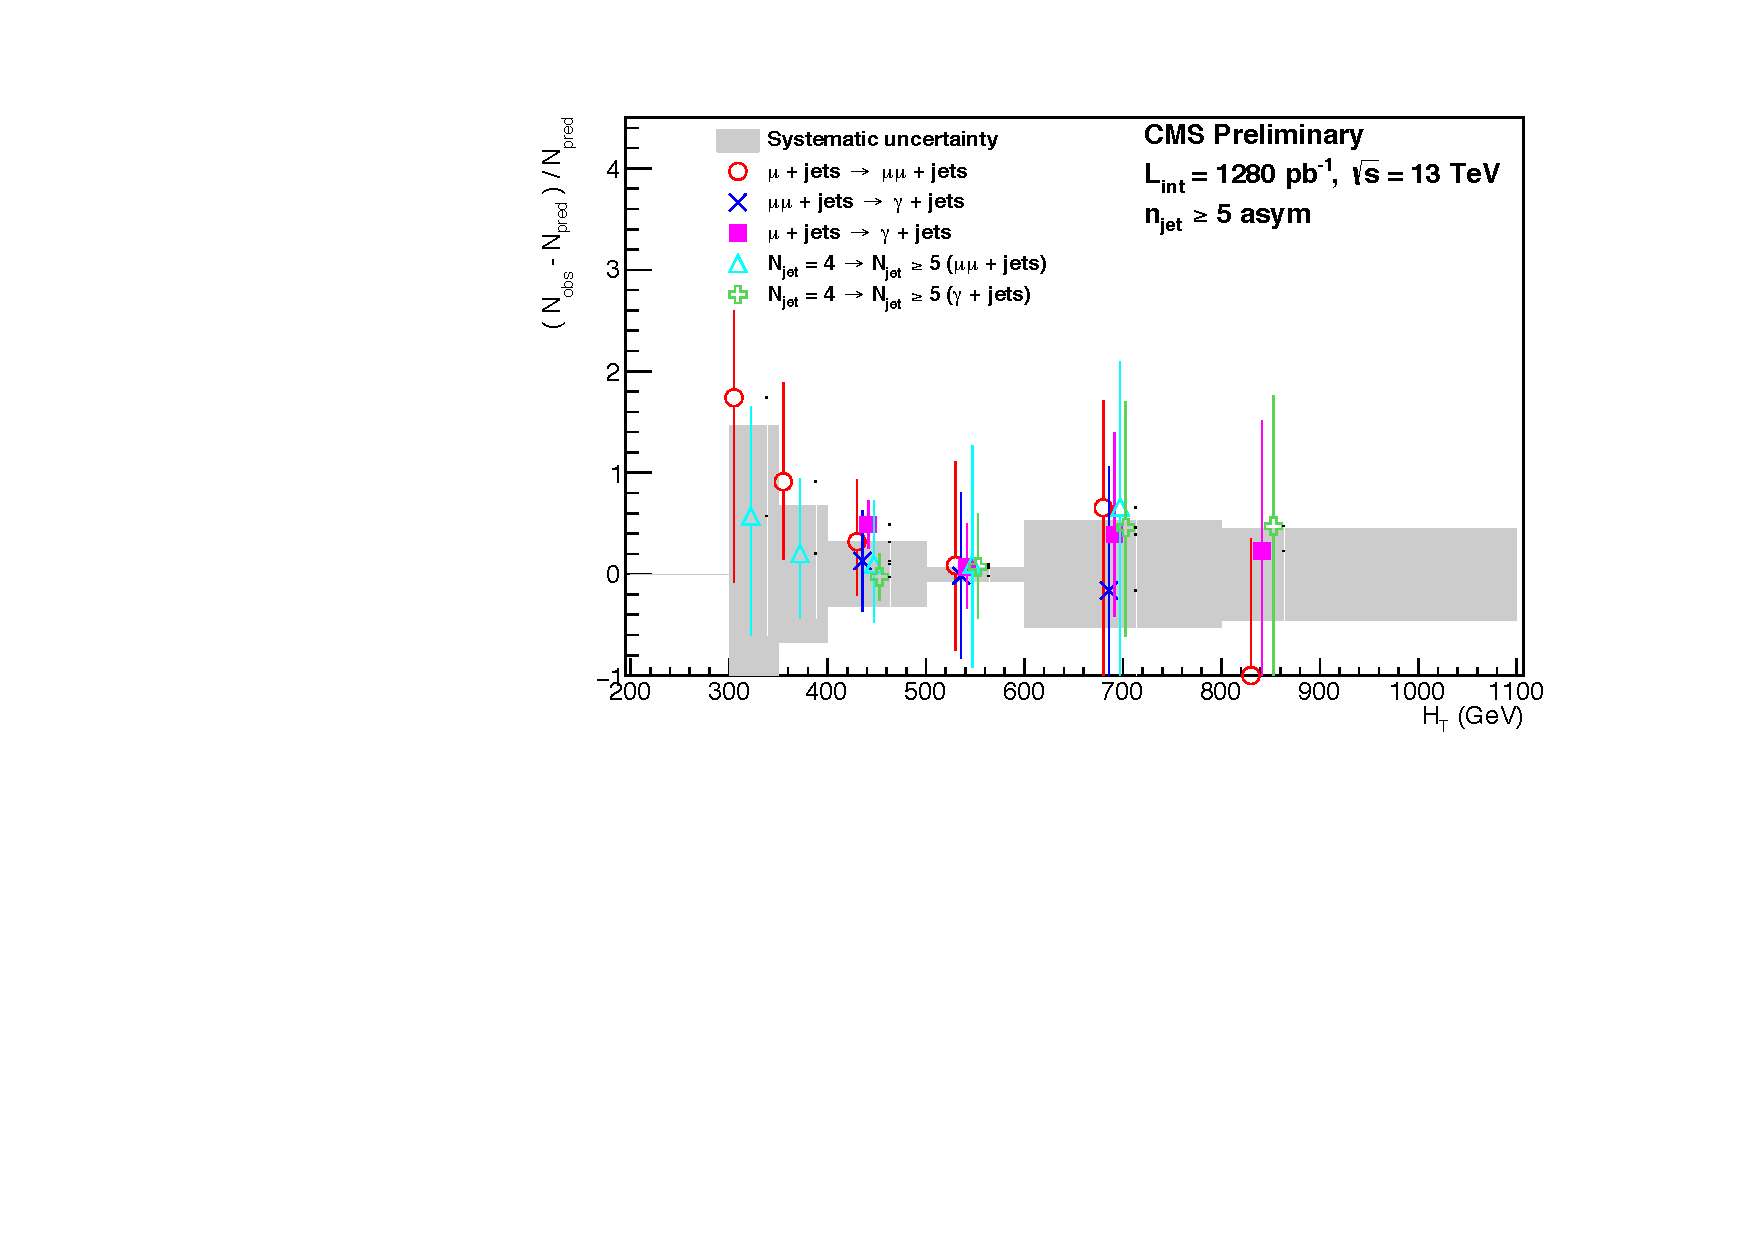
\includegraphics[width=0.5\textwidth]{figures/closureTests/1280pb/Zinv/ge5a.pdf}} \\
%     \caption{Sets of closure tests (open symbols) designed to probe
%       the \znunu + jets overlaid on top of
%       the systematic uncertainty estimates used for each of the seven
%       \scalht bins (shaded bands) carried out with $1.28\ifb$ of
%       $13\tev$ data. All events fit into the ``asymmetric'' jet
%       category}
%     \label{fig:ZinvclosureDataAsym}
%   \end{center} 
% \end{figure}
%
% \begin{figure}[h!]
%   \begin{center}
%     \subfigure[$\njet =
%     1$]{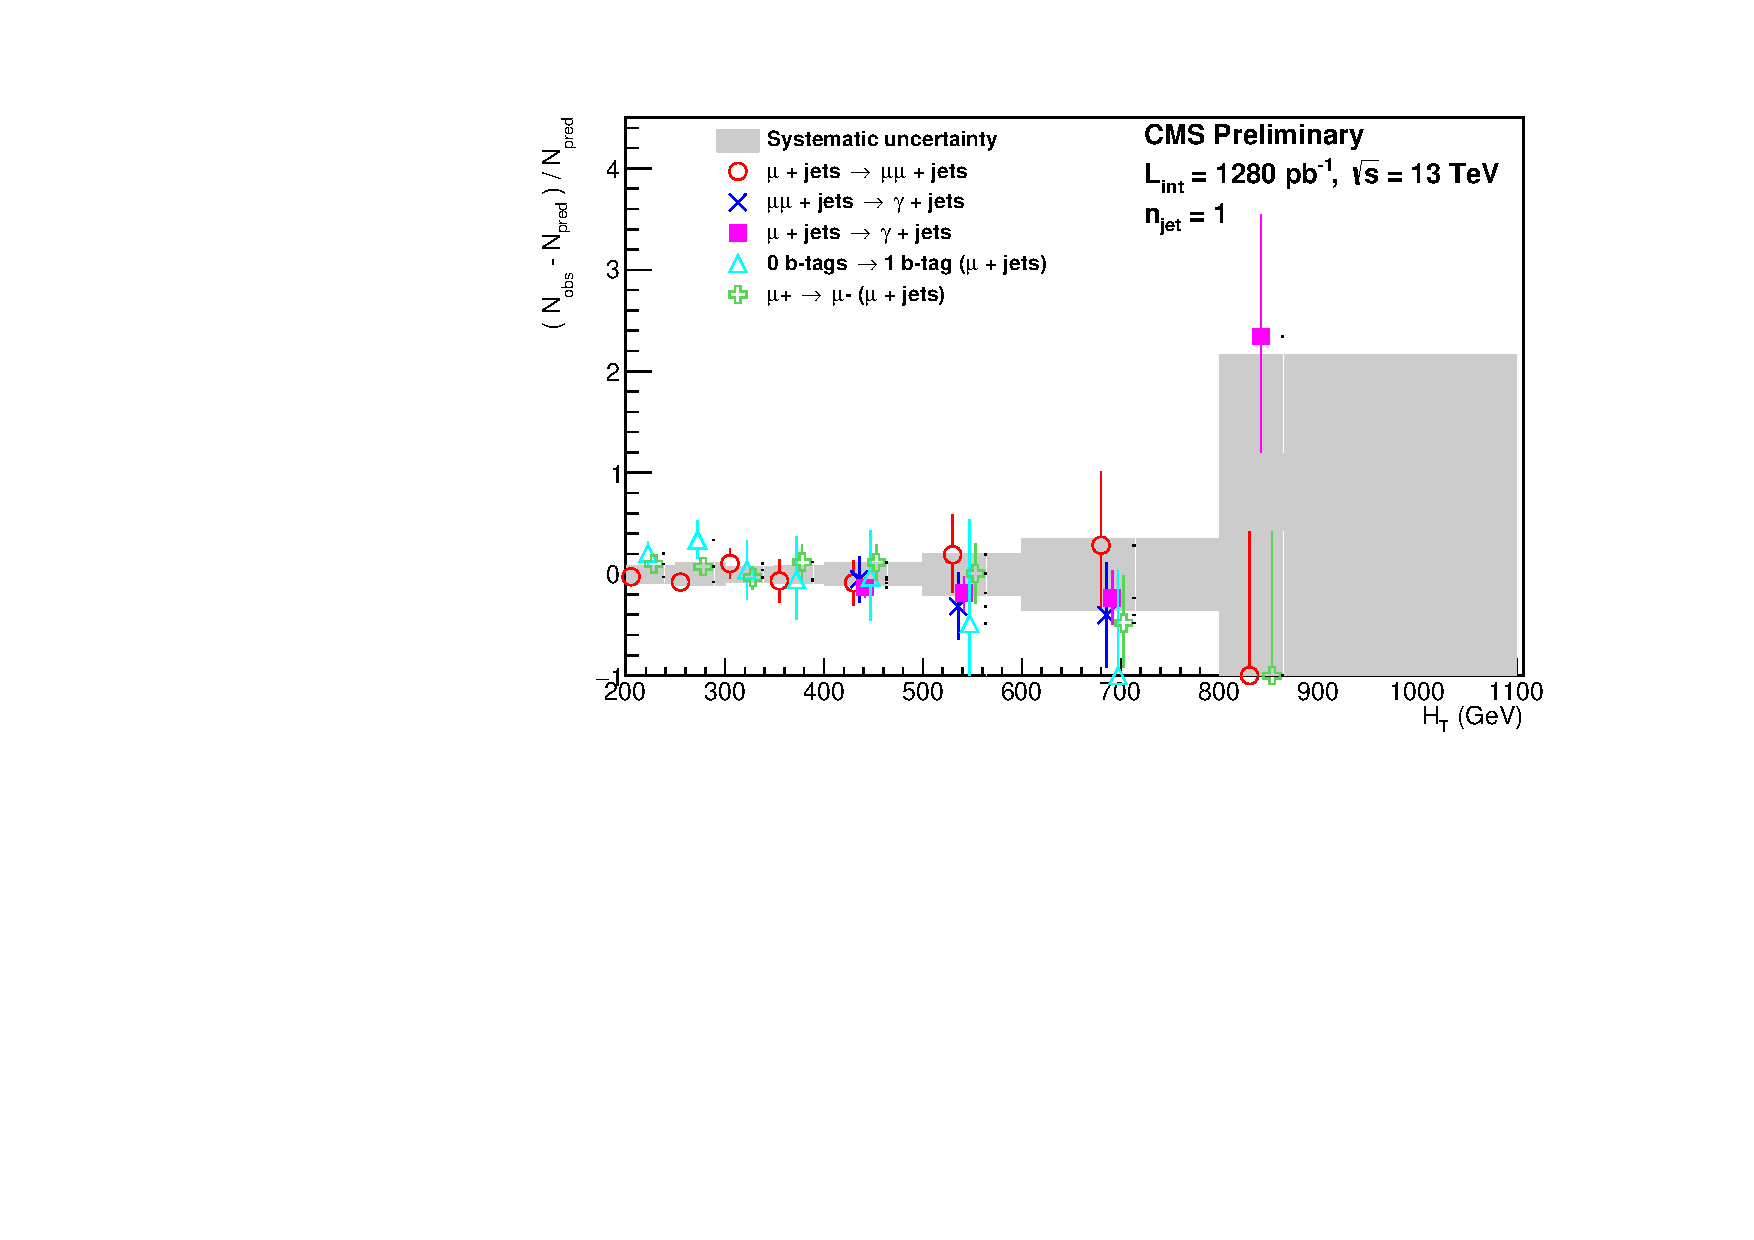
\includegraphics[width=0.7\textwidth]{figures/closureTests/1280pb/eq1j.pdf}} 
%     \caption{Sets of closure tests (open symbols) overlaid on top of
%       the systematic uncertainty estimates used for each of the seven
%       \scalht bins (shaded bands) carried out with $1.28\ifb$ of
%       $13\tev$ data. All events fit into the ``mono-jet'' jet
%       category}
%     \label{fig:closureDataMono}
%   \end{center} 
% \end{figure}
%

%%%%%%%%%%%%%%%%%%%%%%%%%%%%%%%%%%%%%%%%%%%%%%%%%%%%%%%%%%%%%%%%%%%%%%%

With these data studies we calculate the observed systematics as in
Sec.~\ref{sec:syst-from-closure},
this procedure yields the values quoted in
Fig.~\ref{fig:systematicsObs}. In the kinematically restricted bins, such
as those with a high jet multiplicity and low value of \scalht, the
limited statistics leads to large systematic errors. As a minimum number of
events is required for each bin considered in the final stages of the
analysis, these large systematic errors are unlikely to be a problem.
In the bins populated with a reasonable number of events, the
systematic errors determined from the closure tests vary from $10$ to
$40\%$.

The expected systematics, made with the
closure tests detailed in Sec.~\ref{sec:closure-data-study} are also
determined for $1.28\ifb$. These are shown in
Fig.~\ref{fig:systematicsExp}, along with the ratio of observed over
expected systematics. We expect the value of this ratio to remain
close to $1$, with
fluctuations above and below the value. Recall, the
systematic is calculated as the square root of the sum of the weighted
mean squared and weighted variance. When calculating the expected
systematics from MC, the weighted mean is always zero. This is not the
case for the data, we therefore expect the observed systematic to
tend to higher values than the expected systematic. We observe numbers
compatible with this hypothesis, observed divided by expected values
scattered around $1$, with the majority slightly above. 

In addition to
the zero and first order polynomial fits mentioned above, a comparison
of the magnitude of the systematic found in data with that expected
from simulation (\ie in the absence of bias) provides an
additional indication of any genuine bias. The fact
that the observed and expected errors are compatible further supports
the conclusion that there is no extreme source of bias in the closure
tests carried out with data. In the case of bias, we would expect a
much inflated observed systematic.

%%%%%%%%%%%%%%%%%%%%%%%%%%%%%%%%%%%%%%%%%%%%%%%%%%%%%%%%%%%%%%%%%%%%%%%
% table of systematic numbers
%%%%%%%%%%%%%%%%%%%%%%%%%%%%%%%%%%%%%%%%%%%%%%%%%%%%%%%%%%%%%%%%%%%%%%%

\begin{table}[h!]
  \caption{Systematic uncertainties (percent) in the predictions
    of the $\ttbar$W and $\znunu$ (in parentheses) background
    components as a function of \njet, \nb, and \scalht, as determined
    from ensembles of closure tests based on multiple data control
    samples. The data control samples correspond to an integrated
    luminosity of 1.26\fbinv. }
  \label{tab:systs}
  \centering
  \footnotesize
  \begin{tabular}{ ccccccccc }
    \hline
    \hline
    Category & \multicolumn{8}{c}{\scalht bin} \\
    \cline{2-9} 
    
    (\njet,\nb) & 200     & 250     & 300     & 350     & 400     & 500     & 600      & 800       \\
    \hline
    \multicolumn{8}{c}{Monojet:}                                                                   \\
    (1,0)       & 9  (9)  & 12 (12) & 11 (11) & 21 (21) & 11 (11) & 21 (21) & 36 (36)  & -         \\
    (1,1)       & 9  (9)  & 12 (12) & 11 (11) & 21 (21) & 11 (11) & 21 (21) & 36 (36)  & -         \\
    \hline
    \multicolumn{8}{c}{Symmetric:}                                                                 \\
    (2,0)       & 15 (30) & 21 (18) & 15 (16) & 22 (28) & 7 (11)  & 34 (19) & 23 (23)  & 29 (30)   \\
    (2,1)       & 15 (30) & 21 (18) & 15 (16) & 22 (28) & 7 (11)  & 34 (19) & 23 (23)  & 29 (30)   \\
    (2,2)       & 15 (30) & 21 (18) & 15 (16) & 22 (28) & 7 (11)  & 34 (19) & 23 (23)  & 29 (30)   \\
    (3,0)       & 31 (44) & 19 (21) & 15 (27) & 14 (19) & 18 (18) & 14 (13) & 9 (25)   & 24 (17)   \\
    (3,1)       & 31 (44) & 19 (21) & 15 (27) & 14 (19) & 18 (18) & 14 (13) & 9 (25)   & 24 (17)   \\
    (3,2)       & 31 (44) & 19 (21) & 15 (27) & 14 (19) & 18 (18) & 14 (13) & 9 (25)   & 24 (17)   \\
    (3,3)       & 31 (44) & 19 (21) & 15 (27) & 14 (19) & 18 (18) & 14 (13) & 9 (25)   & 24 (17)   \\
    (4,0)       & -       & -       & 36 (34) & 24 (30) & 13 (21) & 22 (27) & 19 (8)   & 14 (18)   \\
    (4,1)       & -       & -       & 36 (34) & 24 (30) & 13 (21) & 22 (27) & 19 (8)   & 14 (18)   \\
    (4,2)       & -       & -       & 36 (34) & 24 (30) & 13 (21) & 22 (27) & 19 (8)   & 14 (18)   \\
    (4,$\geq$3) & -       & -       & 36 (34) & 24 (30) & 13 (21) & 22 (27) & 19 (8)   & 14 (18)   \\
    (5,0)       & -       & -       & -       & 19 (28) & 15 (16) & 19 (34) & 21 (17)  & 22 (19)   \\
    (5,1)       & -       & -       & -       & 19 (28) & 15 (16) & 19 (34) & 21 (17)  & 22 (19)   \\
    (5,2)       & -       & -       & -       & 19 (28) & 15 (16) & 19 (34) & 21 (17)  & 22 (19)   \\
    (5,$\geq$3) & -       & -       & -       & 19 (28) & 15 (16) & 19 (34) & 21 (17)  & 22 (19)   \\
    \hline
    \multicolumn{8}{c}{Asymmetric:}                                                                \\
    (2,0)       & 11 (9)  & 14 (13) & 17 (10) & 14 (11) & 19 (14) & 17 (20) & 105 (46) & 91   (35) \\
    (2,1)       & 11 (9)  & 14 (13) & 17 (10) & 14 (11) & 19 (14) & 17 (20) & 105 (46) & 91   (35) \\
    (2,2)       & 11 (9)  & 14 (13) & 17 (10) & 14 (11) & 19 (14) & 17 (20) & 105 (46) & 91   (35) \\
    (3,0)       & 16 (18) & 12 (12) & 19 (20) & 27 (22) & 20 (8)  & 28 (37) & 86 (78)  & 41   (61) \\
    (3,1)       & 16 (18) & 12 (12) & 19 (20) & 27 (22) & 20 (8)  & 28 (37) & 86 (78)  & 41   (61) \\
    (3,2)       & 16 (18) & 12 (12) & 19 (20) & 27 (22) & 20 (8)  & 28 (37) & 86 (78)  & 41   (61) \\
    (3,3)       & 16 (18) & 12 (12) & 19 (20) & 27 (22) & 20 (8)  & 28 (37) & 86 (78)  & 41   (61) \\
    (4,0)       & -       & 34 (55) & 17 (15) & 16 (13) & 22 (16) & 29 (7)  & 52 (43)  & 112  (67) \\
    (4,1)       & -       & 34 (55) & 17 (15) & 16 (13) & 22 (16) & 29 (7)  & 52 (43)  & 112  (67) \\
    (4,2)       & -       & 34 (55) & 17 (15) & 16 (13) & 22 (16) & 29 (7)  & 52 (43)  & 112  (67) \\
    (4,$\geq$3) & -       & 34 (55) & 17 (15) & 16 (13) & 22 (16) & 29 (7)  & 52 (43)  & 112  (67) \\
    (5,0)       & -       & -       & 36 (73) & 22 (27) & 19 (32) & 47 (7)  & 45 (53)  & 92   (45) \\
    (5,1)       & -       & -       & 36 (73) & 22 (27) & 19 (32) & 47 (7)  & 45 (53)  & 92   (45) \\
    (5,2)       & -       & -       & 36 (73) & 22 (27) & 19 (32) & 47 (7)  & 45 (53)  & 92   (45) \\
    (5,$\geq$3) & -       & -       & 36 (73) & 22 (27) & 19 (32) & 47 (7)  & 45 (53)  & 92   (45) \\
    \hline
    \hline
  \end{tabular}
\end{table}

%%%%%%%%%%%%%%%%%%%%%%%%%%%%%%%%%%%%%%%%%%%%%%%%%%%%%%%%%%%%%%%%%%%%%%%
% FIXME explicitly mention which closure tests went where
%%%%%%%%%%%%%%%%%%%%%%%%%%%%%%%%%%%%%%%%%%%%%%%%%%%%%%%%%%%%%%%%%%%%%%%

\subsubsection{Dedicated \alphat closure test}

\begin{figure}[h!]
  \begin{center}
    \subfigure[$\njet =
    1$]{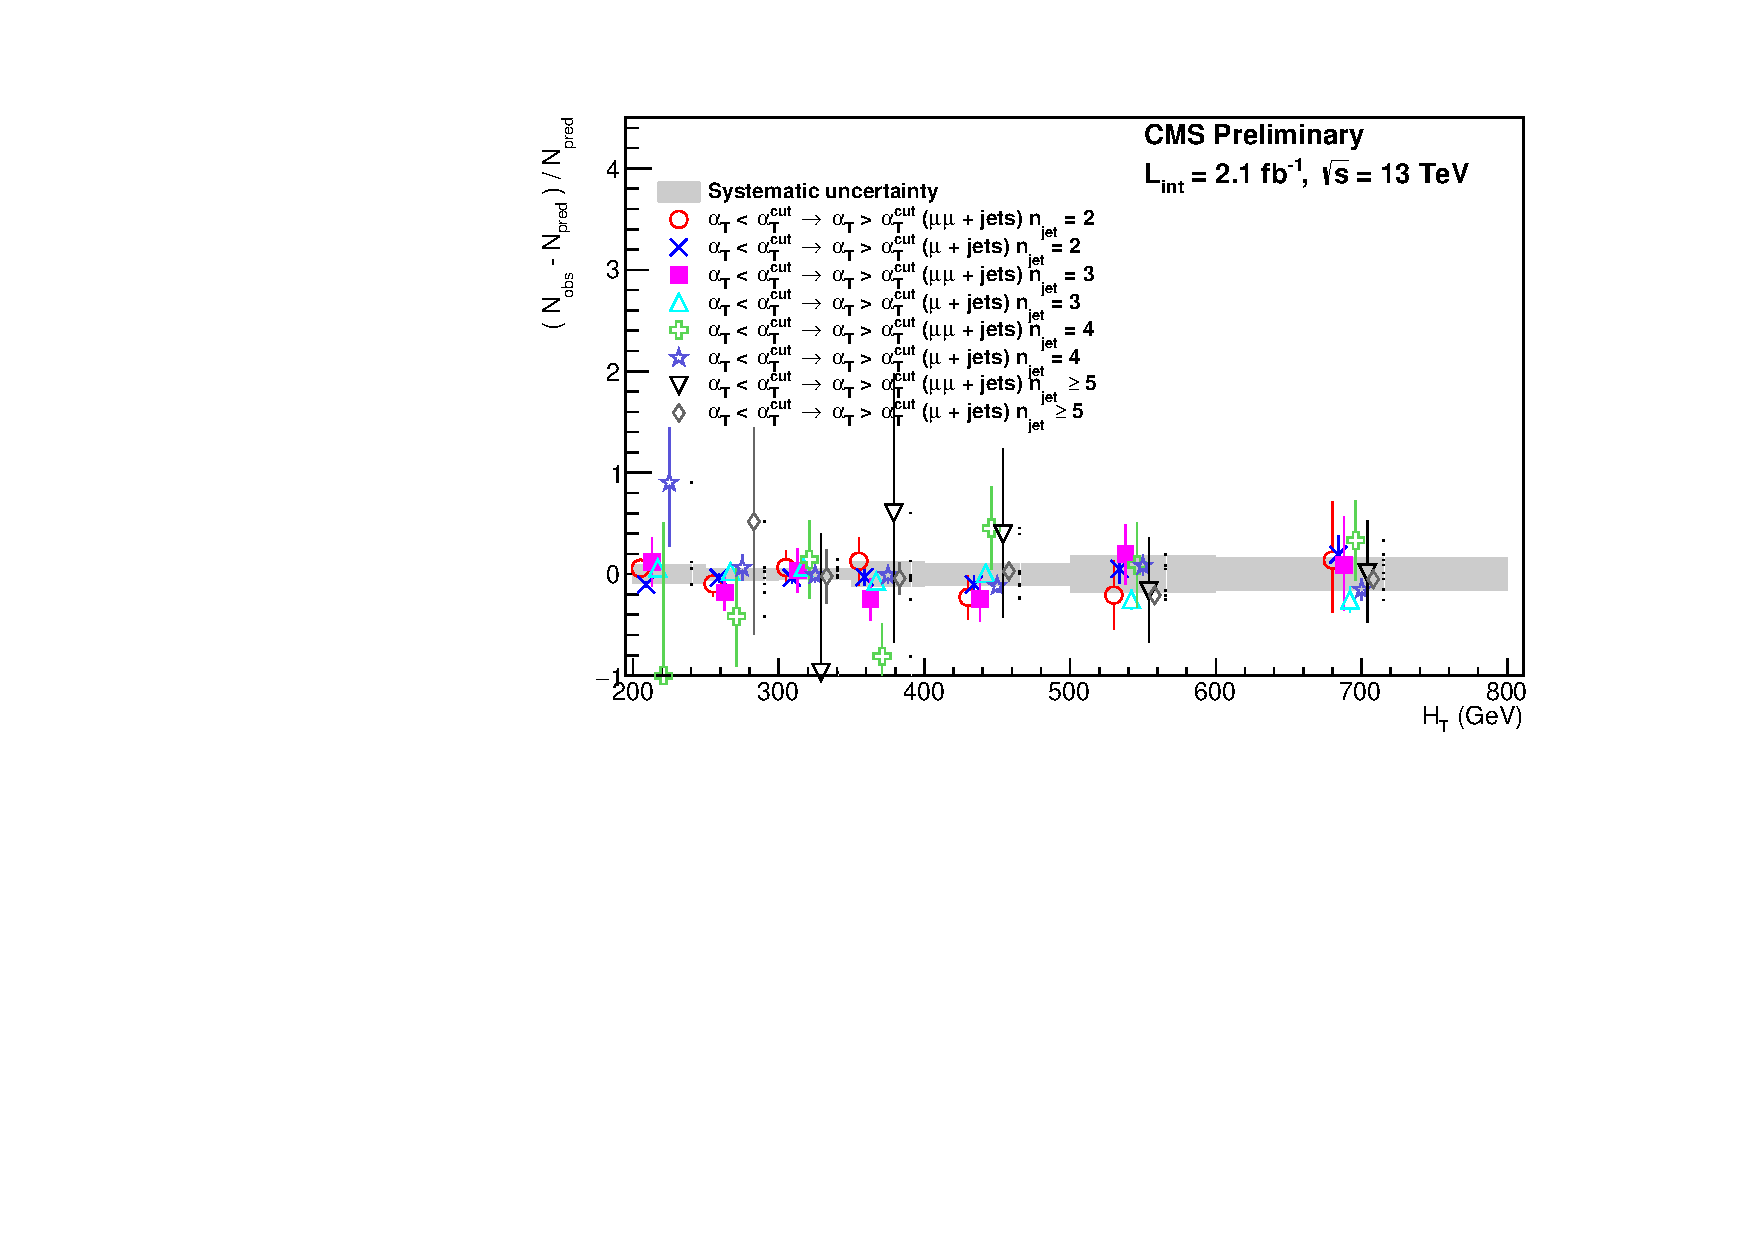
\includegraphics[width=0.7\textwidth]{figures/closureTests/newJamboree/alphaTOnlyTest.pdf}} 
    \caption{Closure tests probing the \alphat extrapolation for each
    \njet category (open symbols) overlaid on top of
      the systematic uncertainty estimates used for each of the seven
      \scalht bins (shaded bands) carried out with $1.28\ifb$ of
      $13\tev$ data. }
    \label{fig:closureAlphaT}
  \end{center} 
\end{figure}

\begin{table}[h!]
  \caption{Systematic uncertainties (percent) in the
    predictions of the $\ttbar$W and $\znunu$ (in parentheses)
    background components as a function of \scalht due to the
    extrapolation in the \alphat (\bdphi) variable in the region
    $\scalht > 800\gev$ ($\scalht > 800\gev$), as determined from
    ensembles of closure tests in multiple data control samples. The
    data control samples correspond to an integrated luminosity of
    1.26\fbinv.} 
  \label{tab:alphaTSyst}
  \centering
  \footnotesize
  \begin{tabular}{ cccccccc }
    \hline
    \hline
    \multicolumn{8}{c}{\scalht bin (GeV)}                                       \\
    \hline
    200   & 250     & 300     & 350     & 400     & 500     & 600     & 800     \\
    8 (8) & 11 (11) & 14 (14) & 15 (15) & 17 (17) & 23 (23) & 25 (25) & 23 (23) \\
    \hline
    \hline
  \end{tabular}
\end{table}


\subsubsection{Closure tests for cross checks}

\begin{figure}[h!]
  \begin{center}
    \subfigure[$\njet =
    1$]{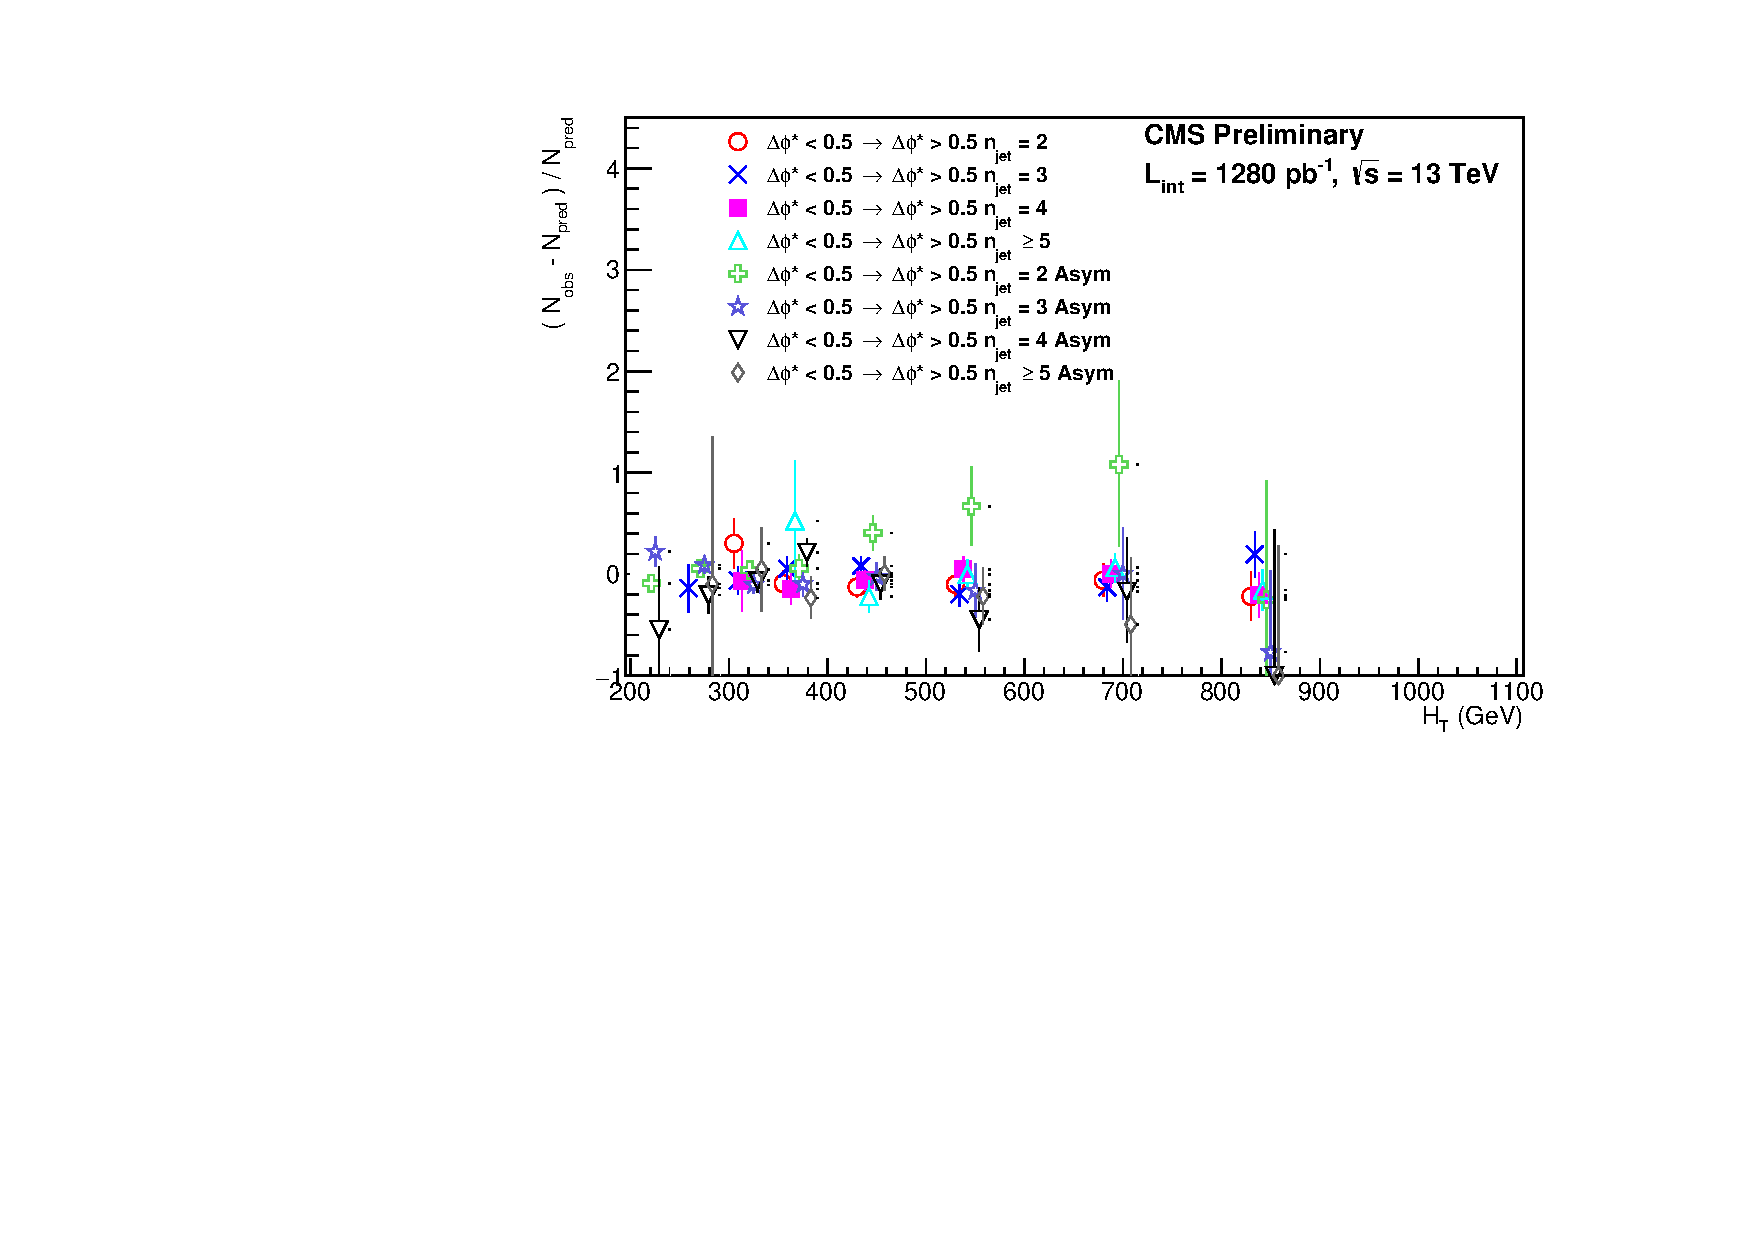
\includegraphics[width=0.7\textwidth]{figures/closureTests/newJamboree/bDPhiCrossCheck.pdf}} 
    \caption{Closure tests probing the $\Delta\phi *$ extrapolation for each
    \njet category (open symbols) carried out with $1.28\ifb$ of
      $13\tev$ data. }
    \label{fig:closureAlphaT}
  \end{center} 
\end{figure}

\begin{figure}[h!]
  \begin{center}
    \subfigure[$\njet =
    1$]{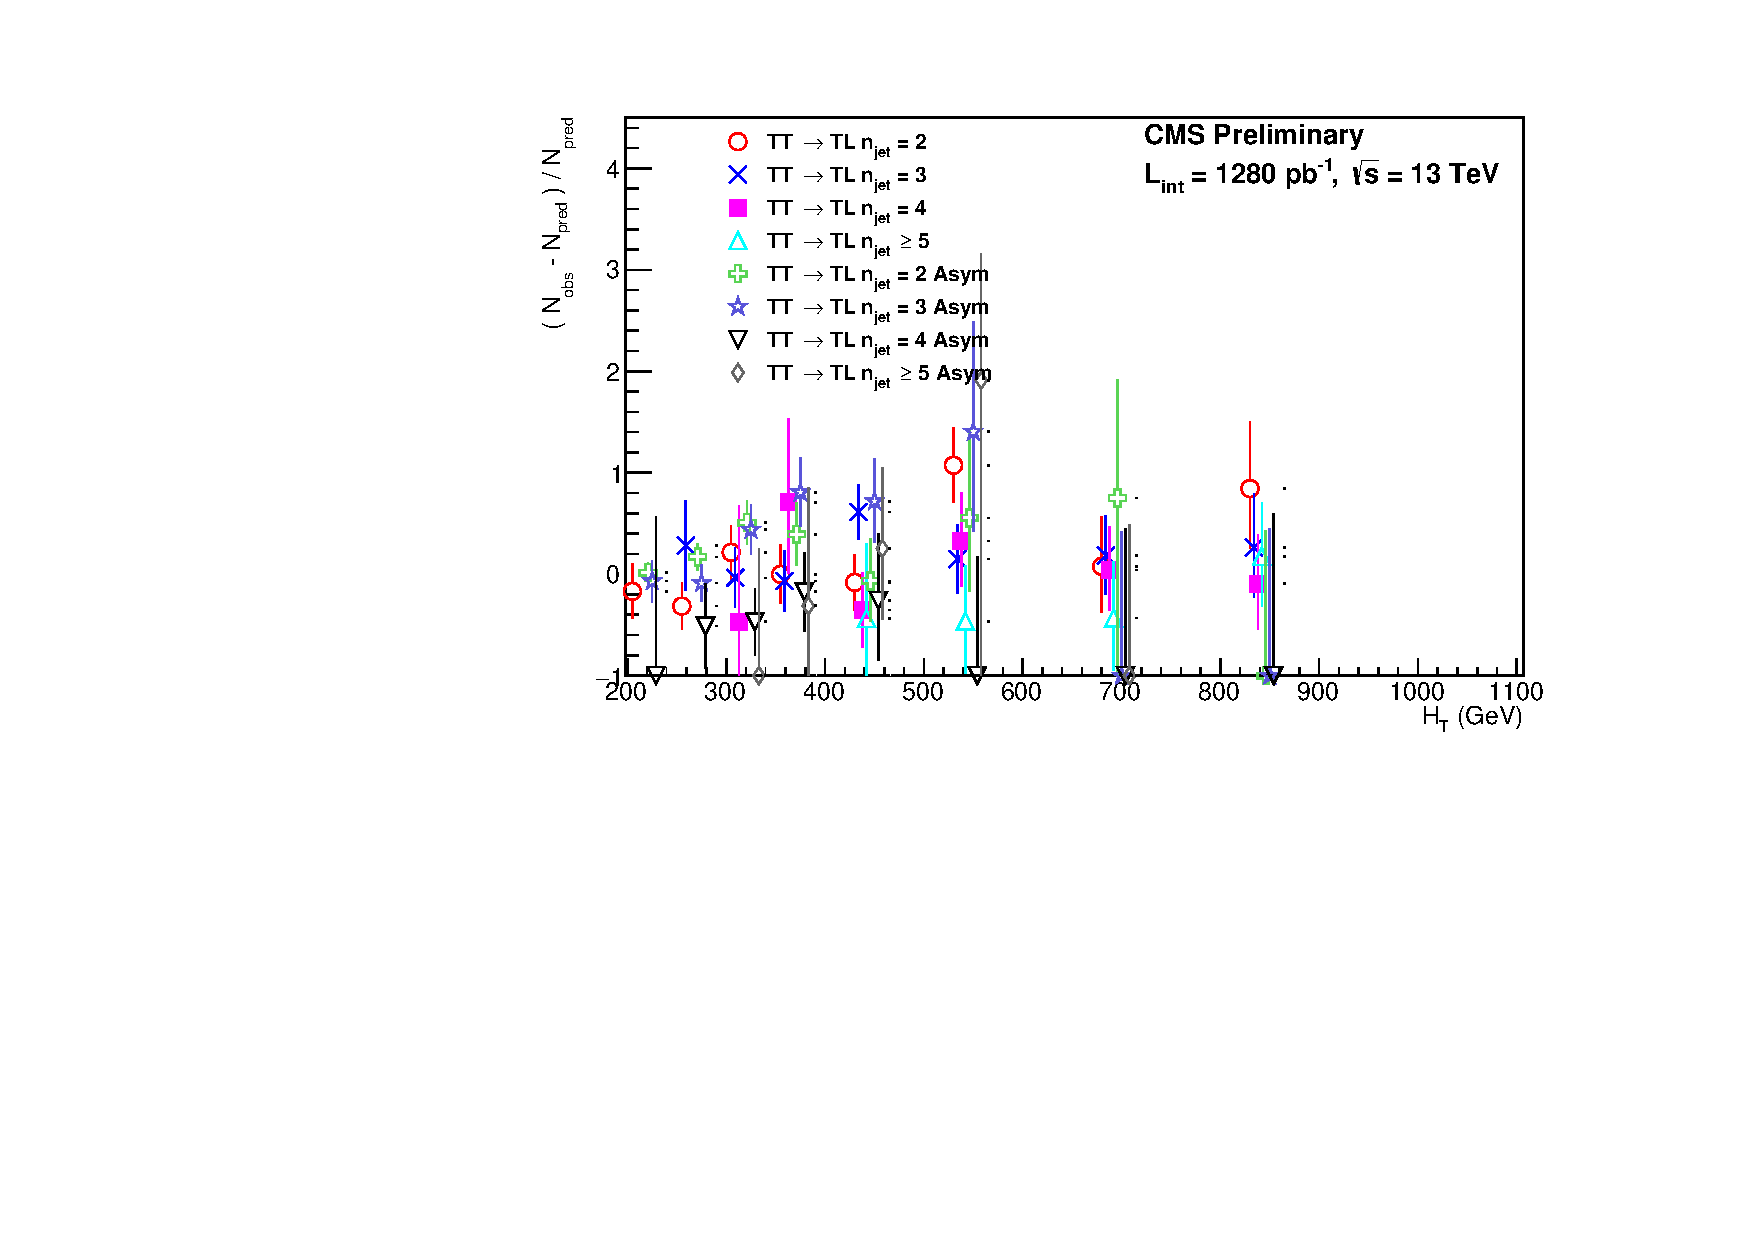
\includegraphics[width=0.7\textwidth]{figures/closureTests/newJamboree/looseLeptonCrossCheck.pdf}} 
    \caption{Closure tests probing the effect of lost leptons in the
    analysis for each
    \njet category (open symbols) carried out with $1.28\ifb$ of
      $13\tev$ data. Events with two muons that pass the control
      region (tight) muon criteria are used to predict events with one
      tight muon and one muon that passes the signal region veto
      criteria (loose)}
    \label{fig:closureAlphaT}
  \end{center} 
\end{figure}



%%%%%%%%%%%%%%%%%%%%%%%%%%%%%%%%%%%%%%%%%%%%%%%%%%%%%%%%%%%%%%%%%%%%%%%
% old 2D plots
%%%%%%%%%%%%%%%%%%%%%%%%%%%%%%%%%%%%%%%%%%%%%%%%%%%%%%%%%%%%%%%%%%%%%%%

% \begin{figure}[]
%   \centering
%   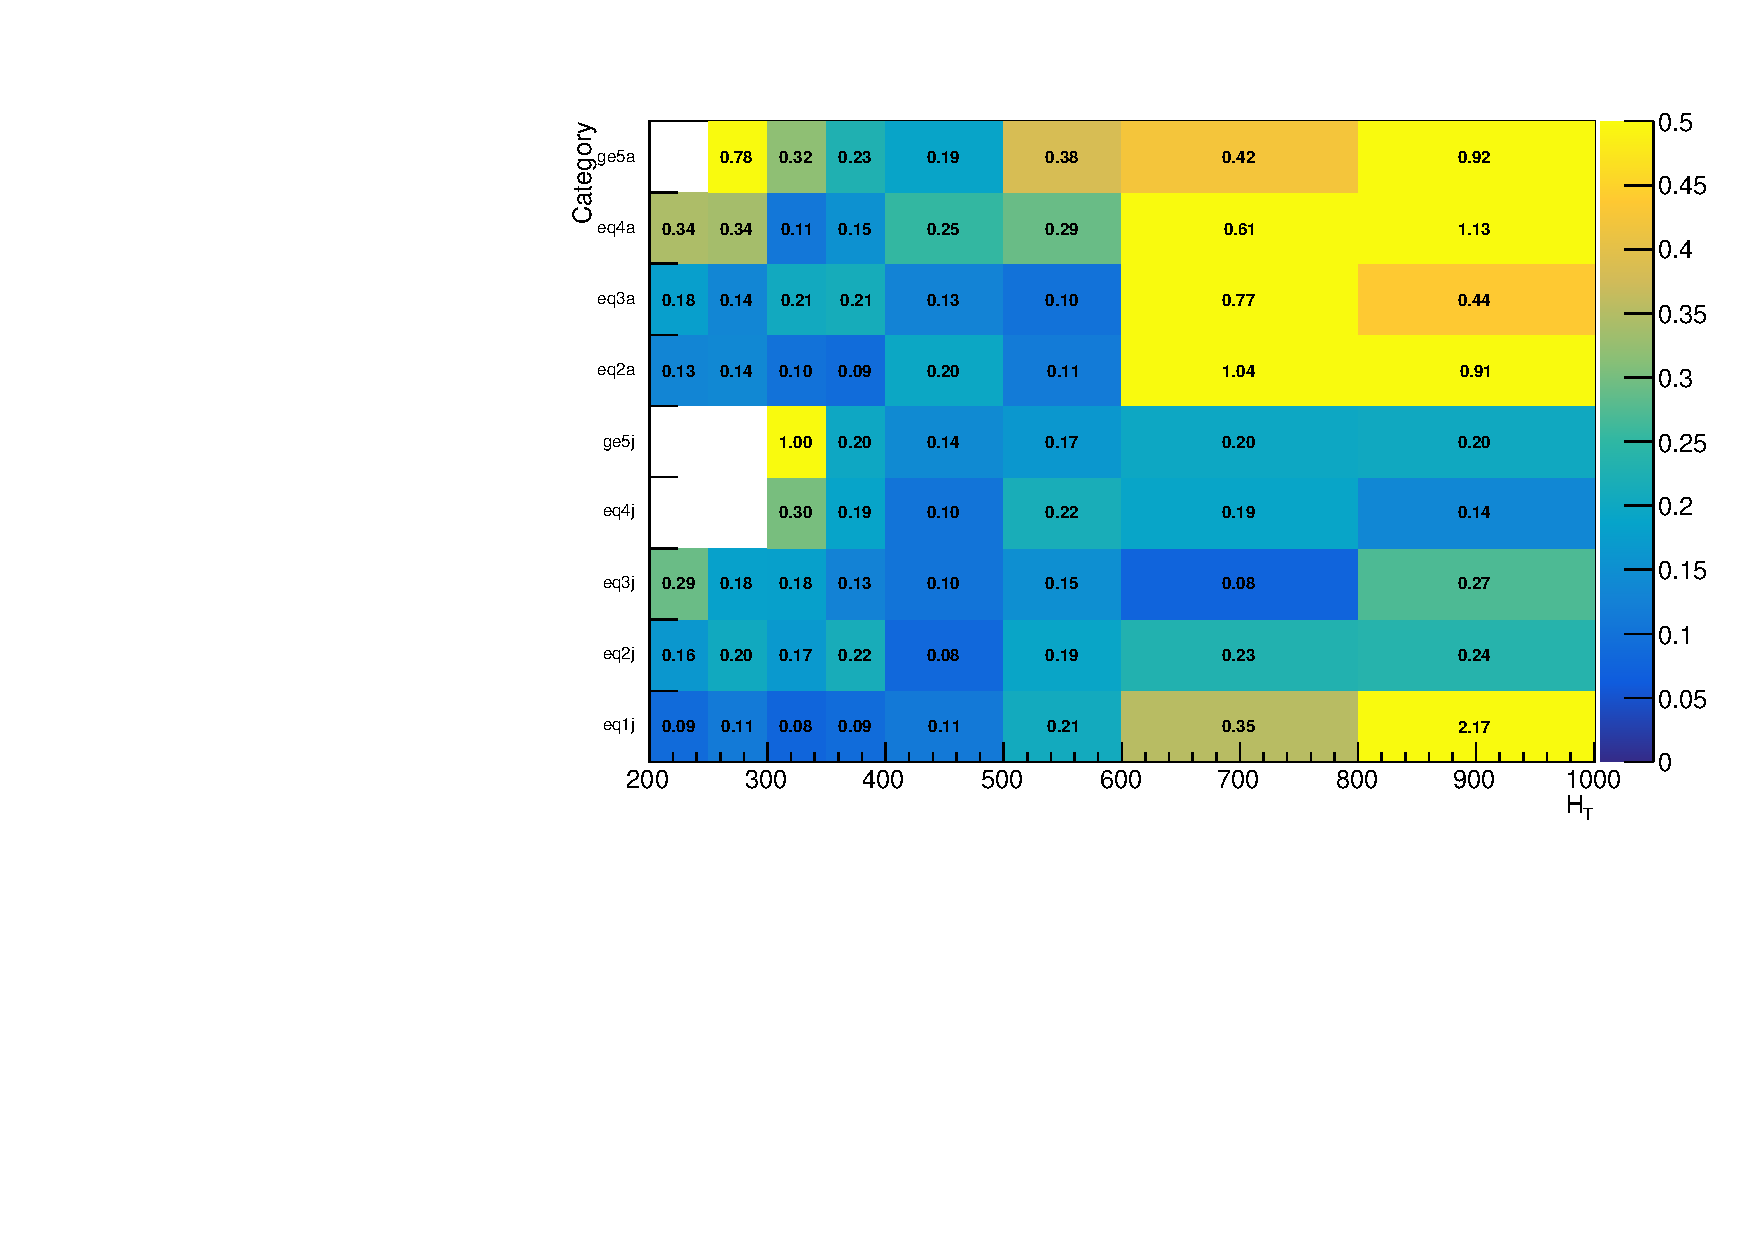
\includegraphics[width=0.7\textwidth]{figures/closureTests/1280pb/ttW/ttW_systOut_obs.pdf}
%   \caption{\label{fig:systematicsObs} Observed systematics for the
%   W and \ttbar + jets background, derived from
%   the closure tests detailed in Sec.~\ref{sec:closure-data-study},
%   made with $1.28\ifb$ of $13\tev$ data with an additional
%   $\mht>130\gev$ requirement.}
% \end{figure}
%
% \begin{figure}[]
%   \centering
%   \subfigure[Expected systematic uncertainties]{
%     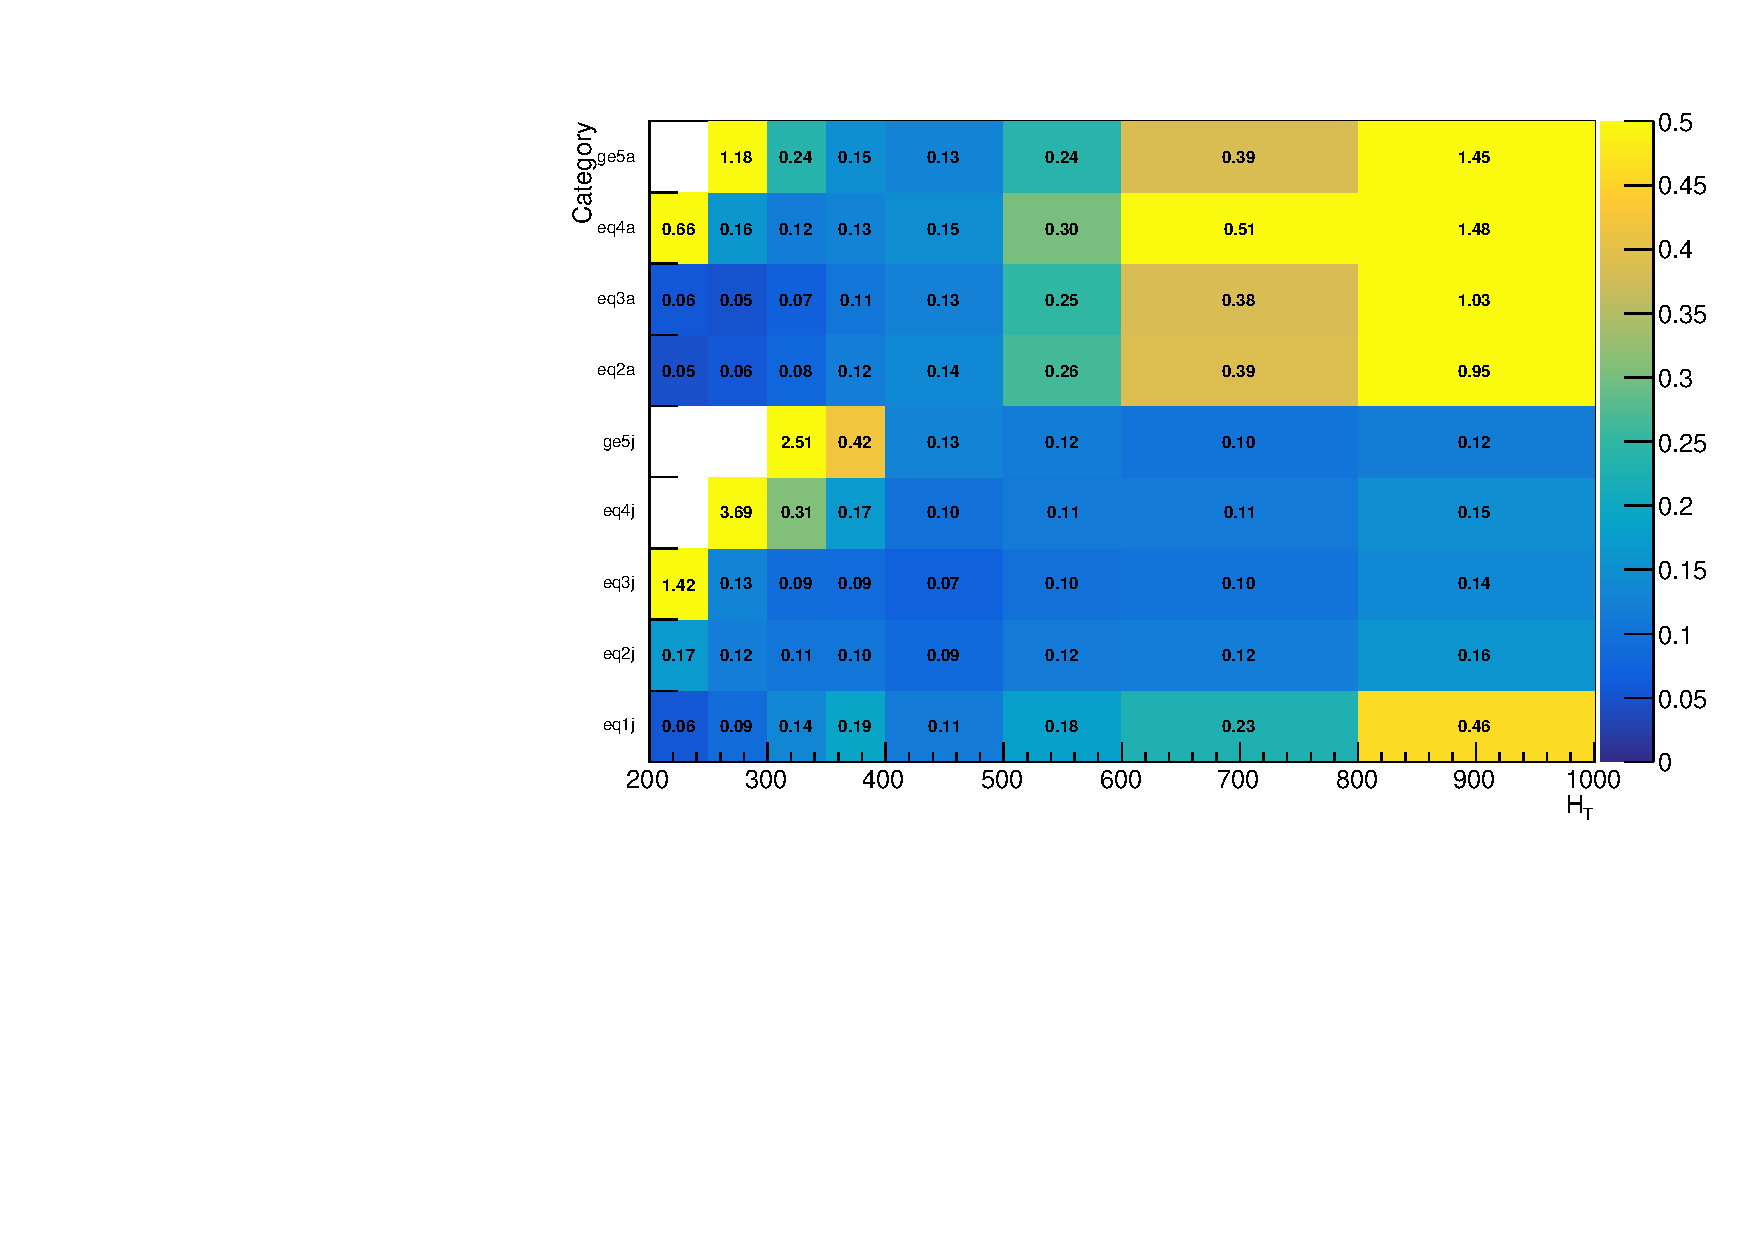
\includegraphics[width=0.5\textwidth]{figures/closureTests/1280pb/ttW/ttW_systOut_exp.pdf}
%   } ~~
%   \subfigure[Observed divided by expected systematic uncertainties]{
%     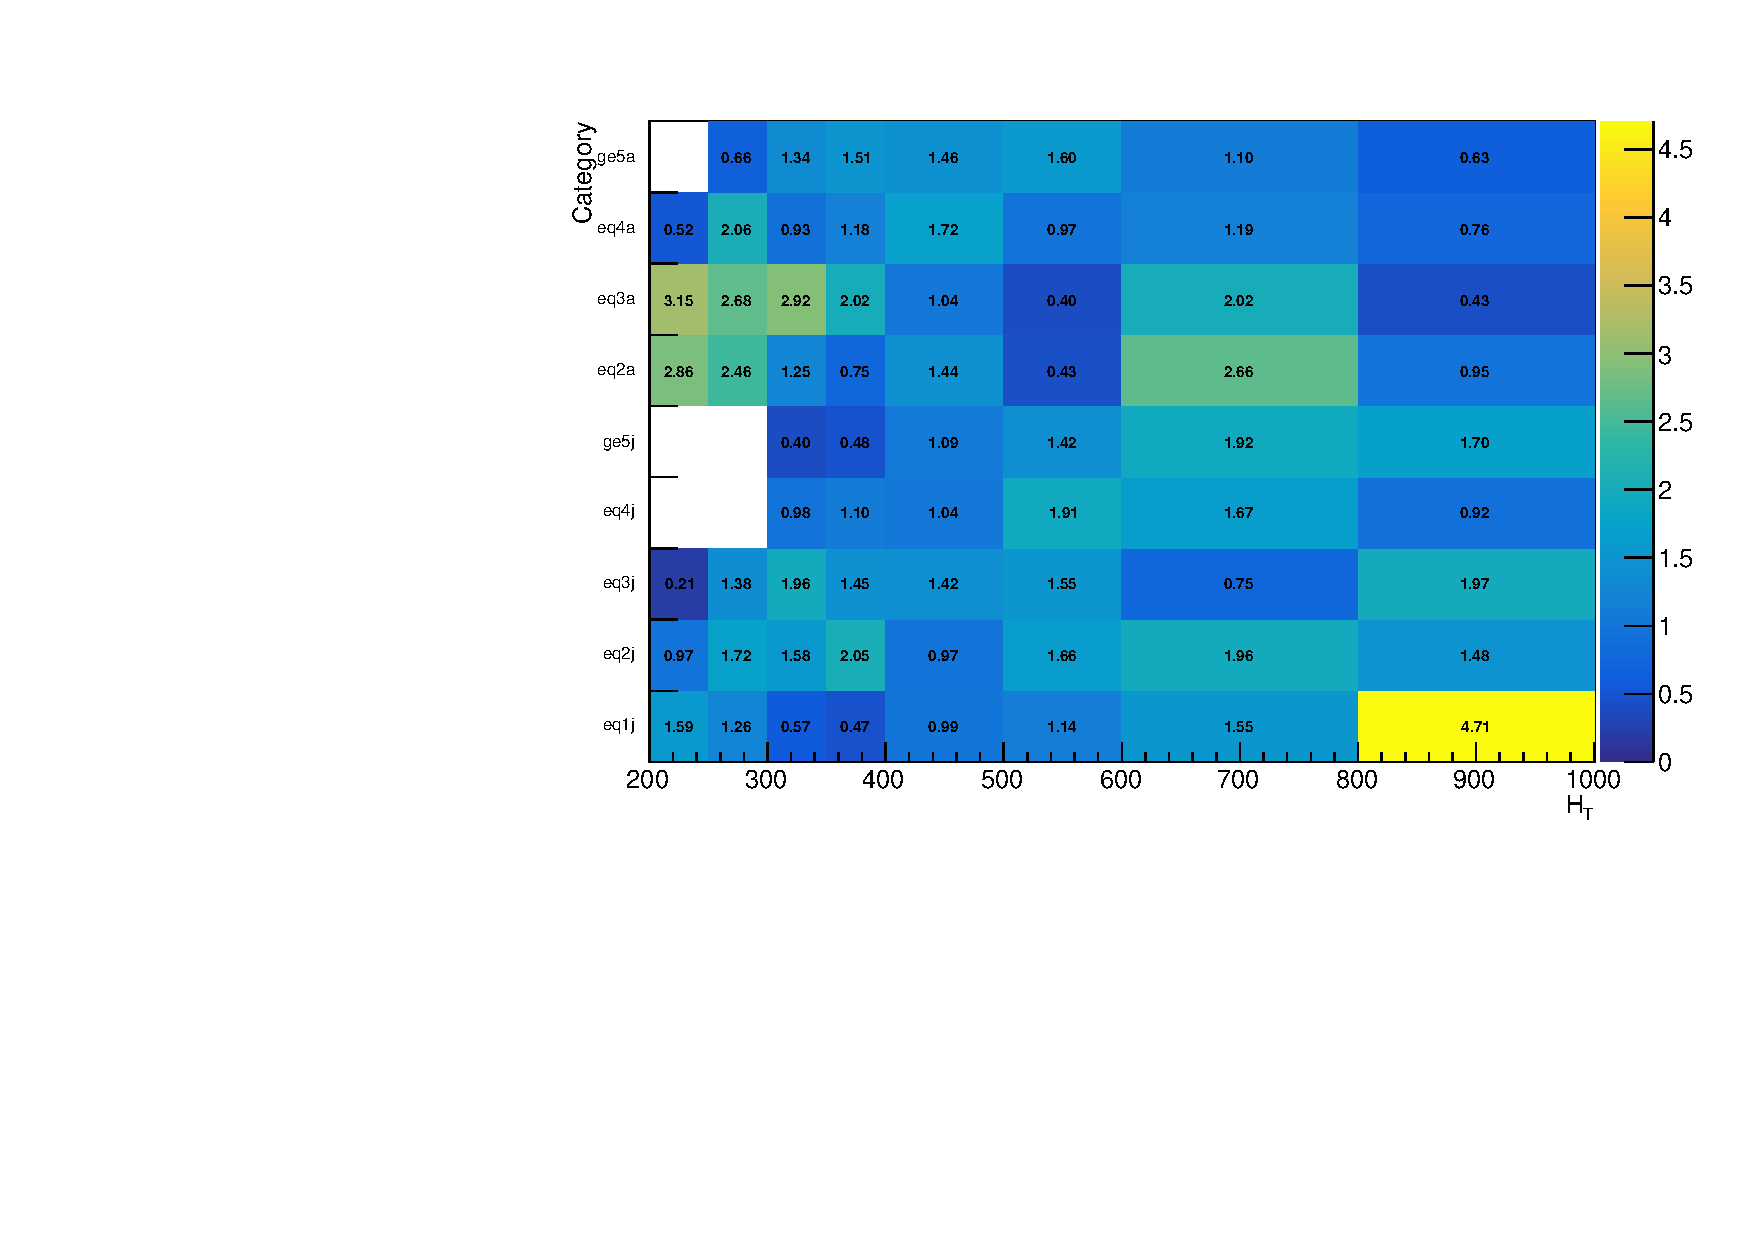
\includegraphics[width=0.5\textwidth]{figures/closureTests/1280pb/ttW/systCompTtW.pdf}
%   }
%   \caption{\label{fig:systematicsExp} Expected systematics and observed
%   (see in Fig~\ref{fig:systematicsObs})
%   divided by expected systematics. Derived from the closure tests 
%   detailed in Sec~\ref{sec:closure-data-study} designed to probe the
%   W and \ttbar + jets background and made with an extra
%   $\mht>130\gev$ requirement. Expected systematics made with MC
%   scaled to $1.28\ifb$}
% \end{figure}
%
% \begin{figure}[]
%   \centering
%   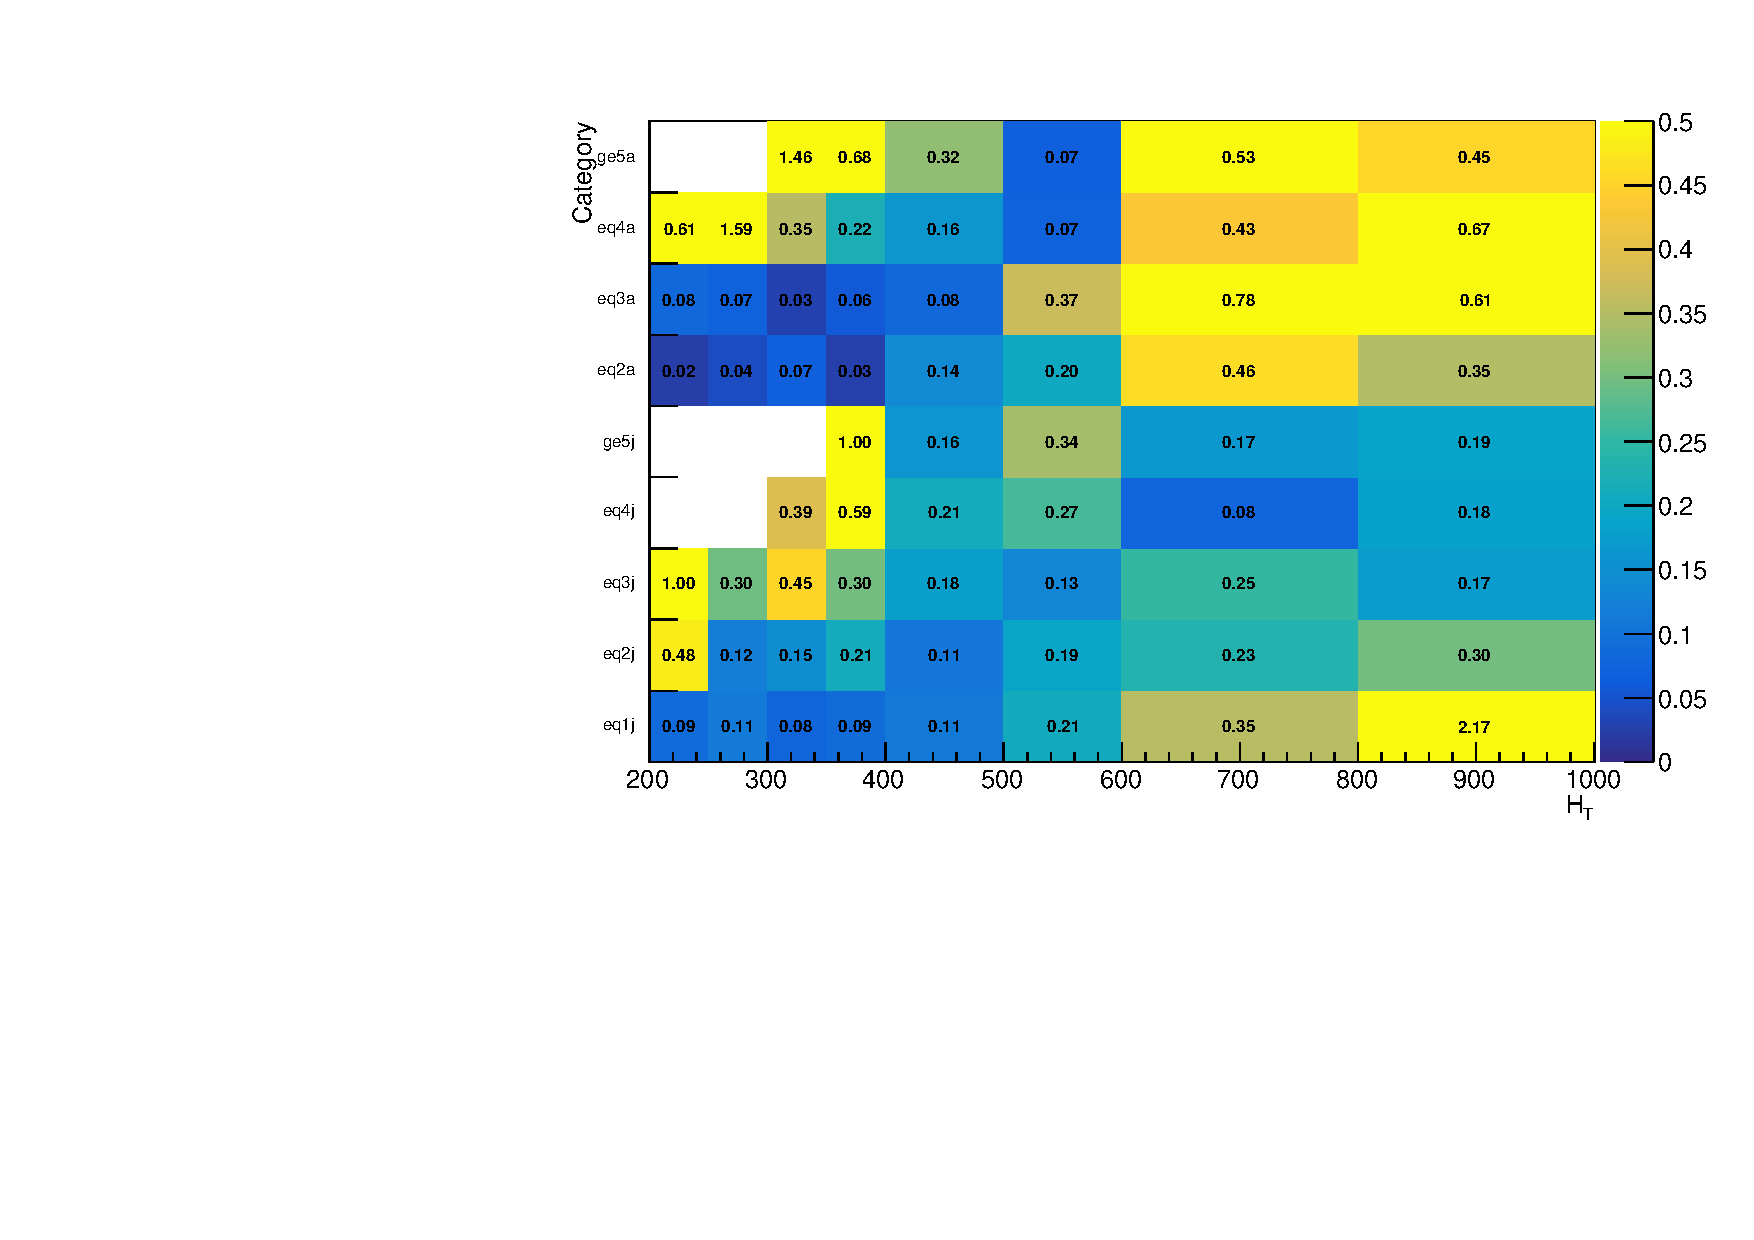
\includegraphics[width=0.7\textwidth]{figures/closureTests/1280pb/Zinv/Zinv_systOut_obs.pdf}
%   \caption{\label{fig:systematicsObs} Observed systematics for the
%   \znunu + jets background, derived from
%   the closure tests detailed in Sec.~\ref{sec:closure-data-study},
%   made with $1.28\ifb$ of $13\tev$ data with an additional
%   $\mht>130\gev$ requirement.}
% \end{figure}
%
% \begin{figure}[]
%   \centering
%   \subfigure[Expected systematic uncertainties]{
%     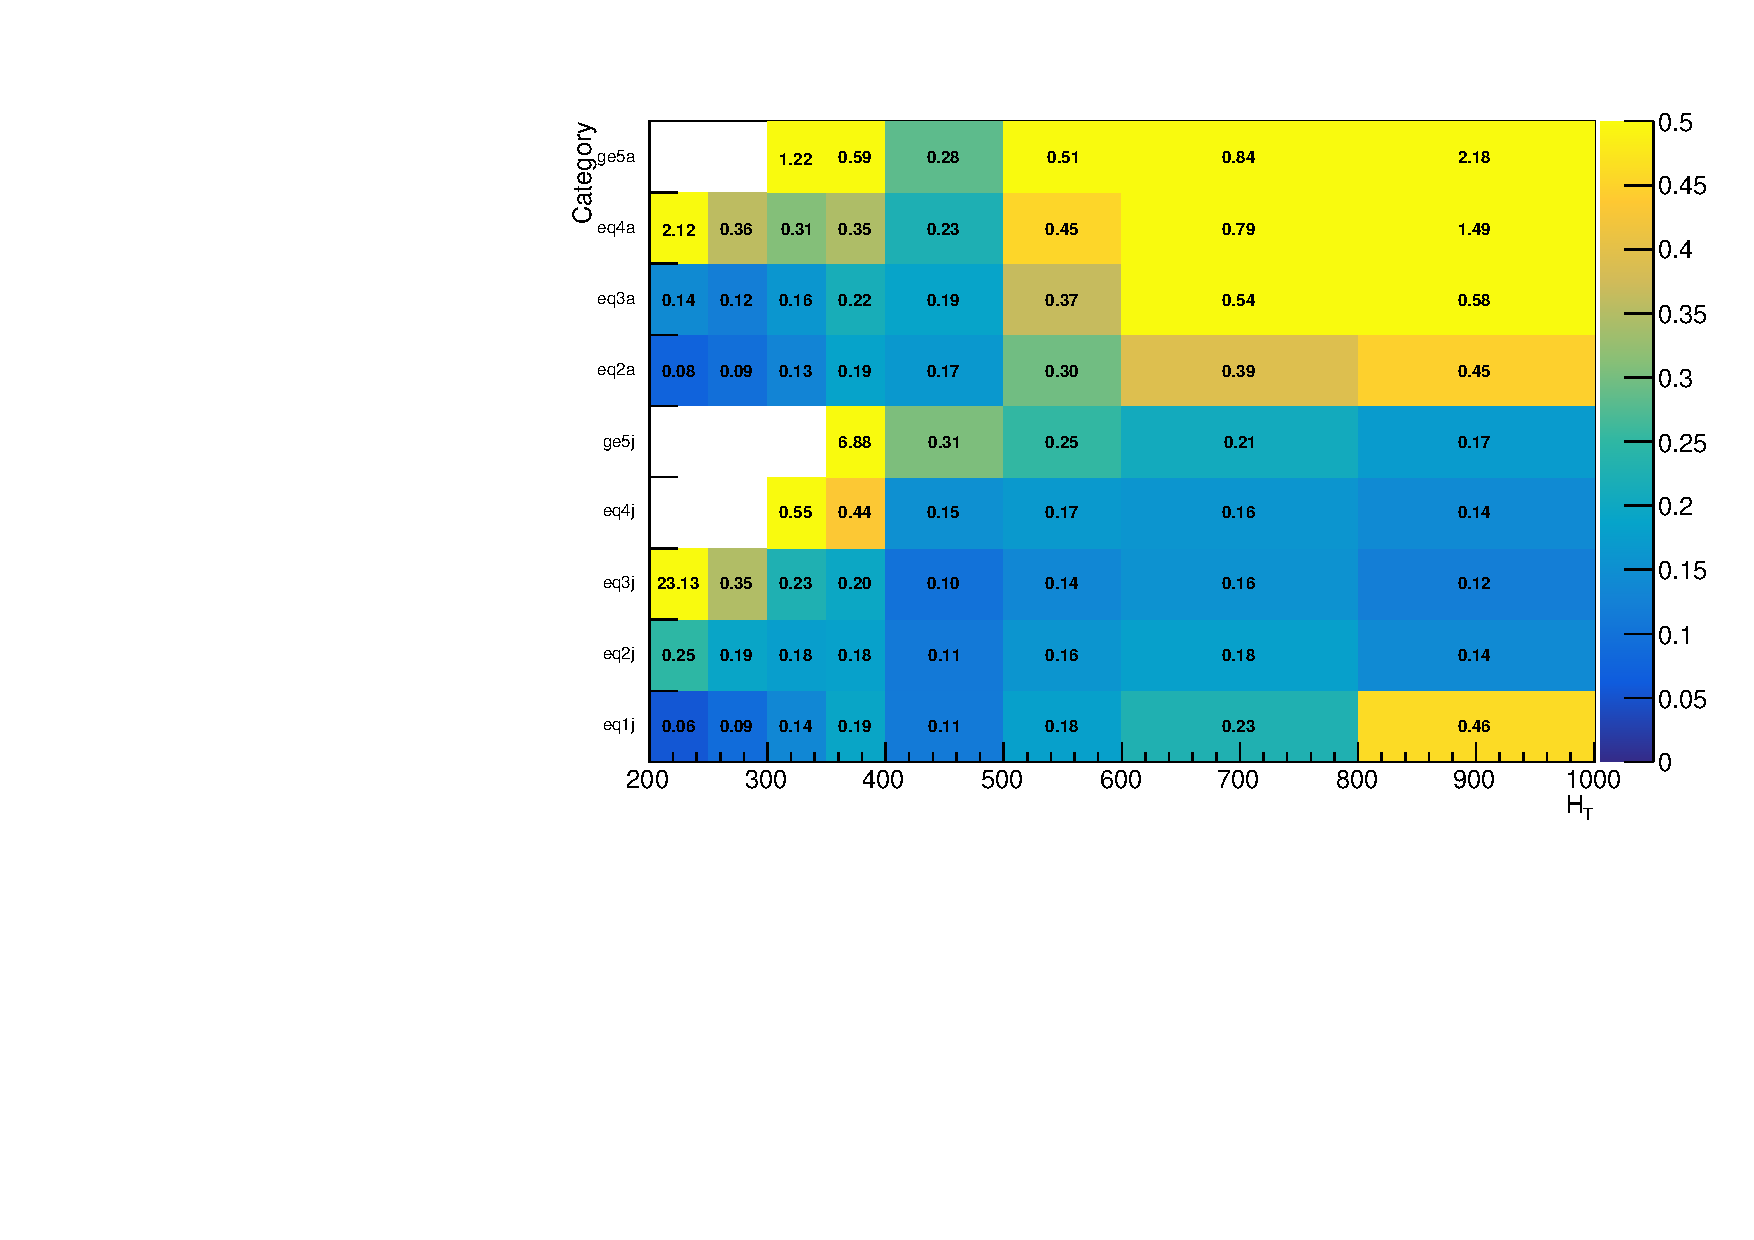
\includegraphics[width=0.5\textwidth]{figures/closureTests/1280pb/Zinv/Zinv_systOut_exp.pdf}
%   } ~~
%   \subfigure[Observed divided by expected systematic uncertainties]{
%     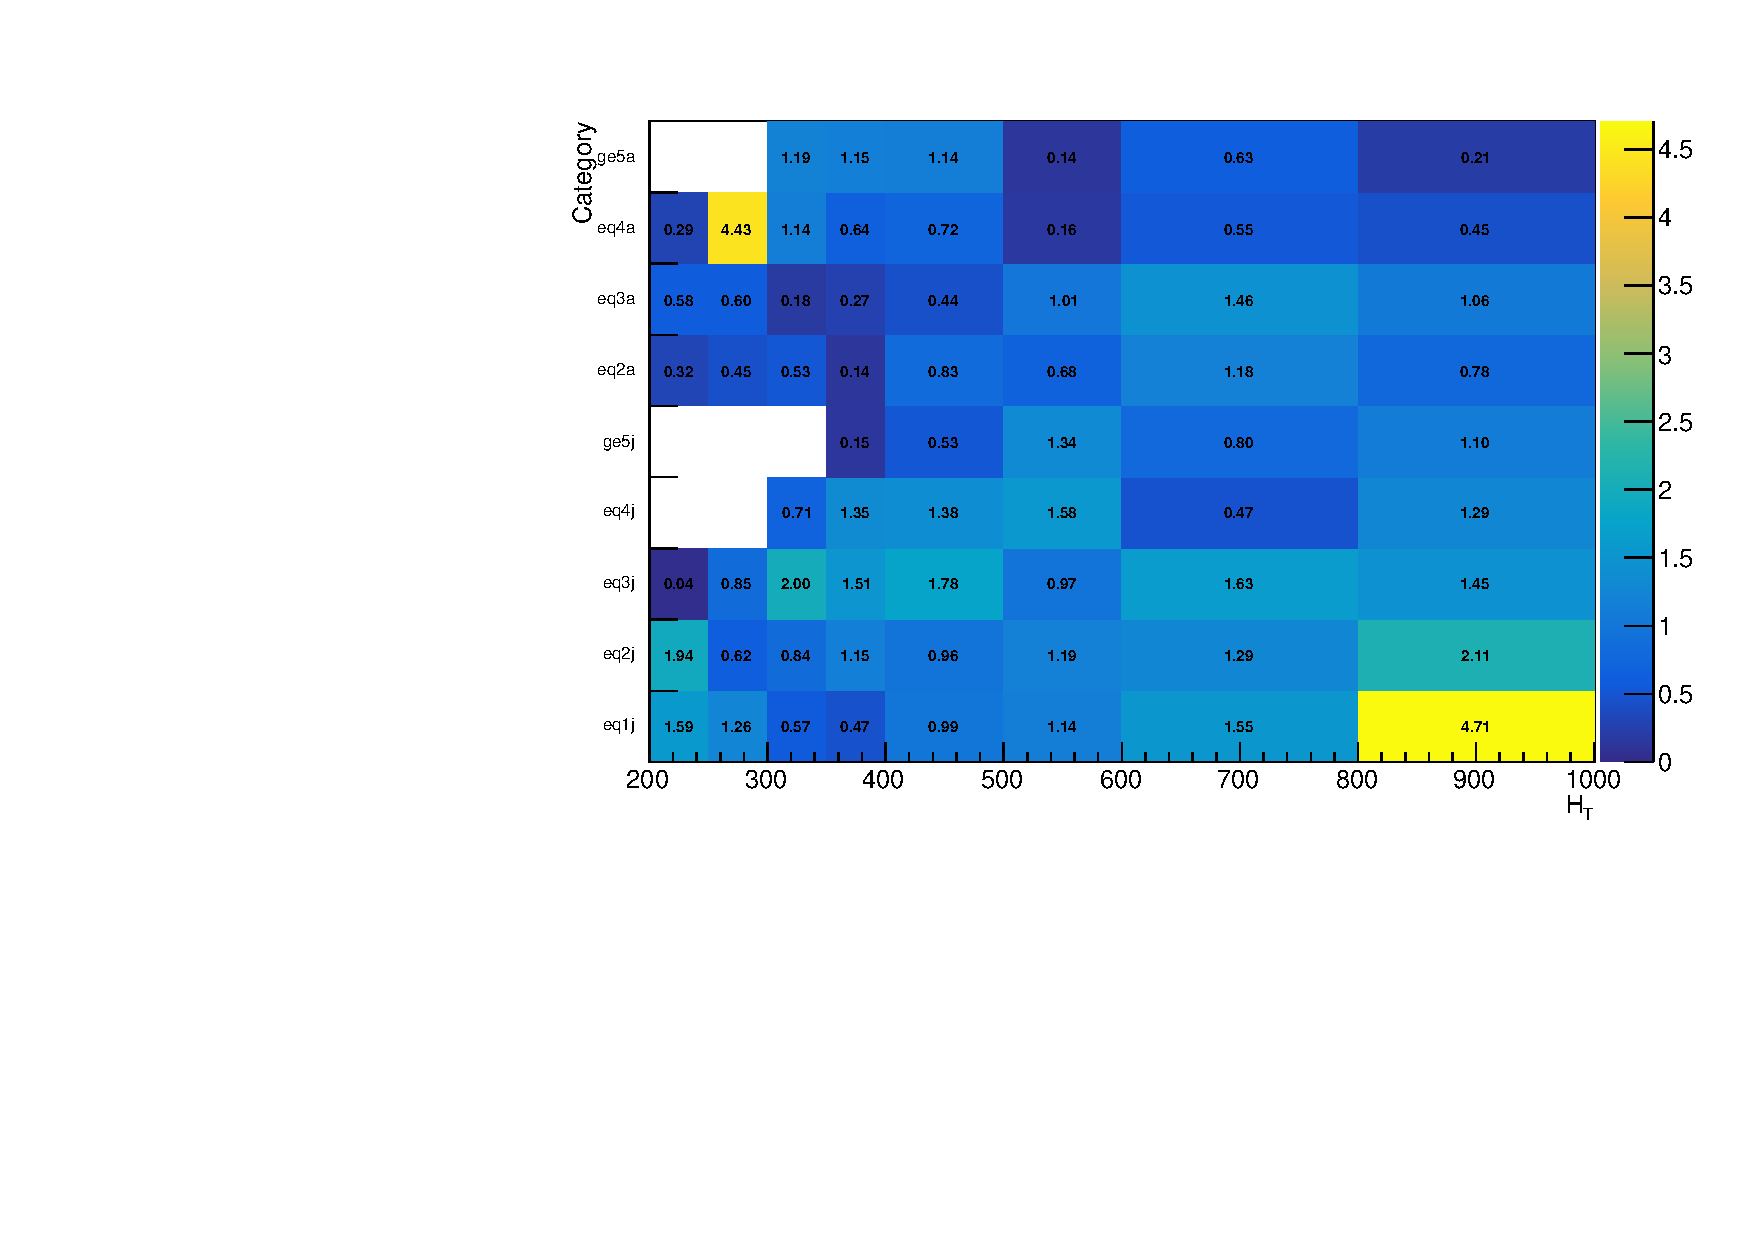
\includegraphics[width=0.5\textwidth]{figures/closureTests/1280pb/Zinv/systCompZinv.pdf}
%   }
%   \caption{\label{fig:systematicsExp} Expected systematics and observed
%   (see in Fig~\ref{fig:systematicsObs})
%   divided by expected systematics. Derived from the closure tests 
%   detailed in Sec~\ref{sec:closure-data-study} designed to probe the
%   \znunu + jets background and made with an extra
%   $\mht>130\gev$ requirement. Expected systematics made with MC
%   scaled to $1.28\ifb$}
% \end{figure}

\subsection{Monte Carlo systematic uncertainties in transfer factors}
\label{sec:mc-systematics}

As described in Secs.~\ref{sec:backgroundmet} and~\ref{sec:closure-tests-desc},
the non-multijet background yields per $(\njet,\nb,\scalht)$
bin are estimated through the use of control regions and
appropriate MC-based transfer factors. This approach aims to minimise
the sensitivity to simulation mismodelling, as many systematic biases are
expected to cancel to a large extent in the ratios defining the transfer
factors. Systematic uncertainties on the transfer factors accounting for
residual biases are derived from the data-driven closure tests.

We still consider a wide range of  systematic effects arising from 
uncertainties in jet energy scales, b-tag scale factors, parton distribution 
functions, lepton and photon identification, etc. These are all expected 
to be sub-dominant with respect to the systematic uncertainties derived 
from the closure tests, and we check that this is the case.

The procedure to determine the effect of these sources of systematic
uncertainties is to construct the transfer factors when varying in turn each
source by their up and down one sigma uncertainties, and express this as a
percentage difference relative to the nominal transfer factors. 

These sources of systematic uncertainty can affect both the
experimental acceptance of the signal and control regions, as well as event
migration between analysis bins. The former is accounted for by cross section
corrections derived from sidebands and NNLO calculations. The aim in this case
is to assess the relative changes in the transfer factors across bins
as the variations are performed and the overall integrated yields are fixed.

%{\bf Jet energy corrections}

As a preliminary study, the effect of varying the jet
energy scale in the \mj and \mmj control regions is investigated.
The energies of jets used in the analysis are corrected as a function of
their \pt and $\eta$ via the procedure recommended by
the JetMET POG. These corrections have an associated uncertainty,
which can propagate through the analysis. 
As the analysis is designed such that bins
with the same value of \scalht and jet multiplicity in the control
regions are used to predict the background in the signal region, we
expect to be protected against many of the effects caused by these jet
energy scale uncertainties. However, the jet energy scale can still
have an effect, due to jets moving in and
out acceptance (above and below $40\gev$).

Full selection, as described in Sec.~\ref{sec:selection}, is required.
If any control region bin has fewer
than $1$ predicted events at $1280\ipb$ it is left out of the study.
Pseudo transfer factors are calculated in each analysis bin, defined
as the number of events in a signal region after passing the signal
region \alphat cut in a particular bin divided by the total number of
events in that bin. This is carried out using the jet energy
corrections with their nominal, most likely, value and with their
minus one sigma, lower bound, value. The relative change in these two
transfer factors is then calculated. For the \mj control region, these
values are shown in Fig.~\ref{fig:jes-syst-singleMu}. For the \mmj
control region, these values are shown in
Fig.~\ref{fig:jes-syst-doubleMu}. 

Overall, the effect of varying the jet energy scale down appears to be
small. With variations in the pseudo transfer factors being typically
less than $10\%$. Any larger effects are likely due to statistical
fluctuations in bins with a small number of events.


\begin{figure}[]
  \centering
  \subfigure[The relative change in transfer factors per \scalht bin
  and jet category]{
    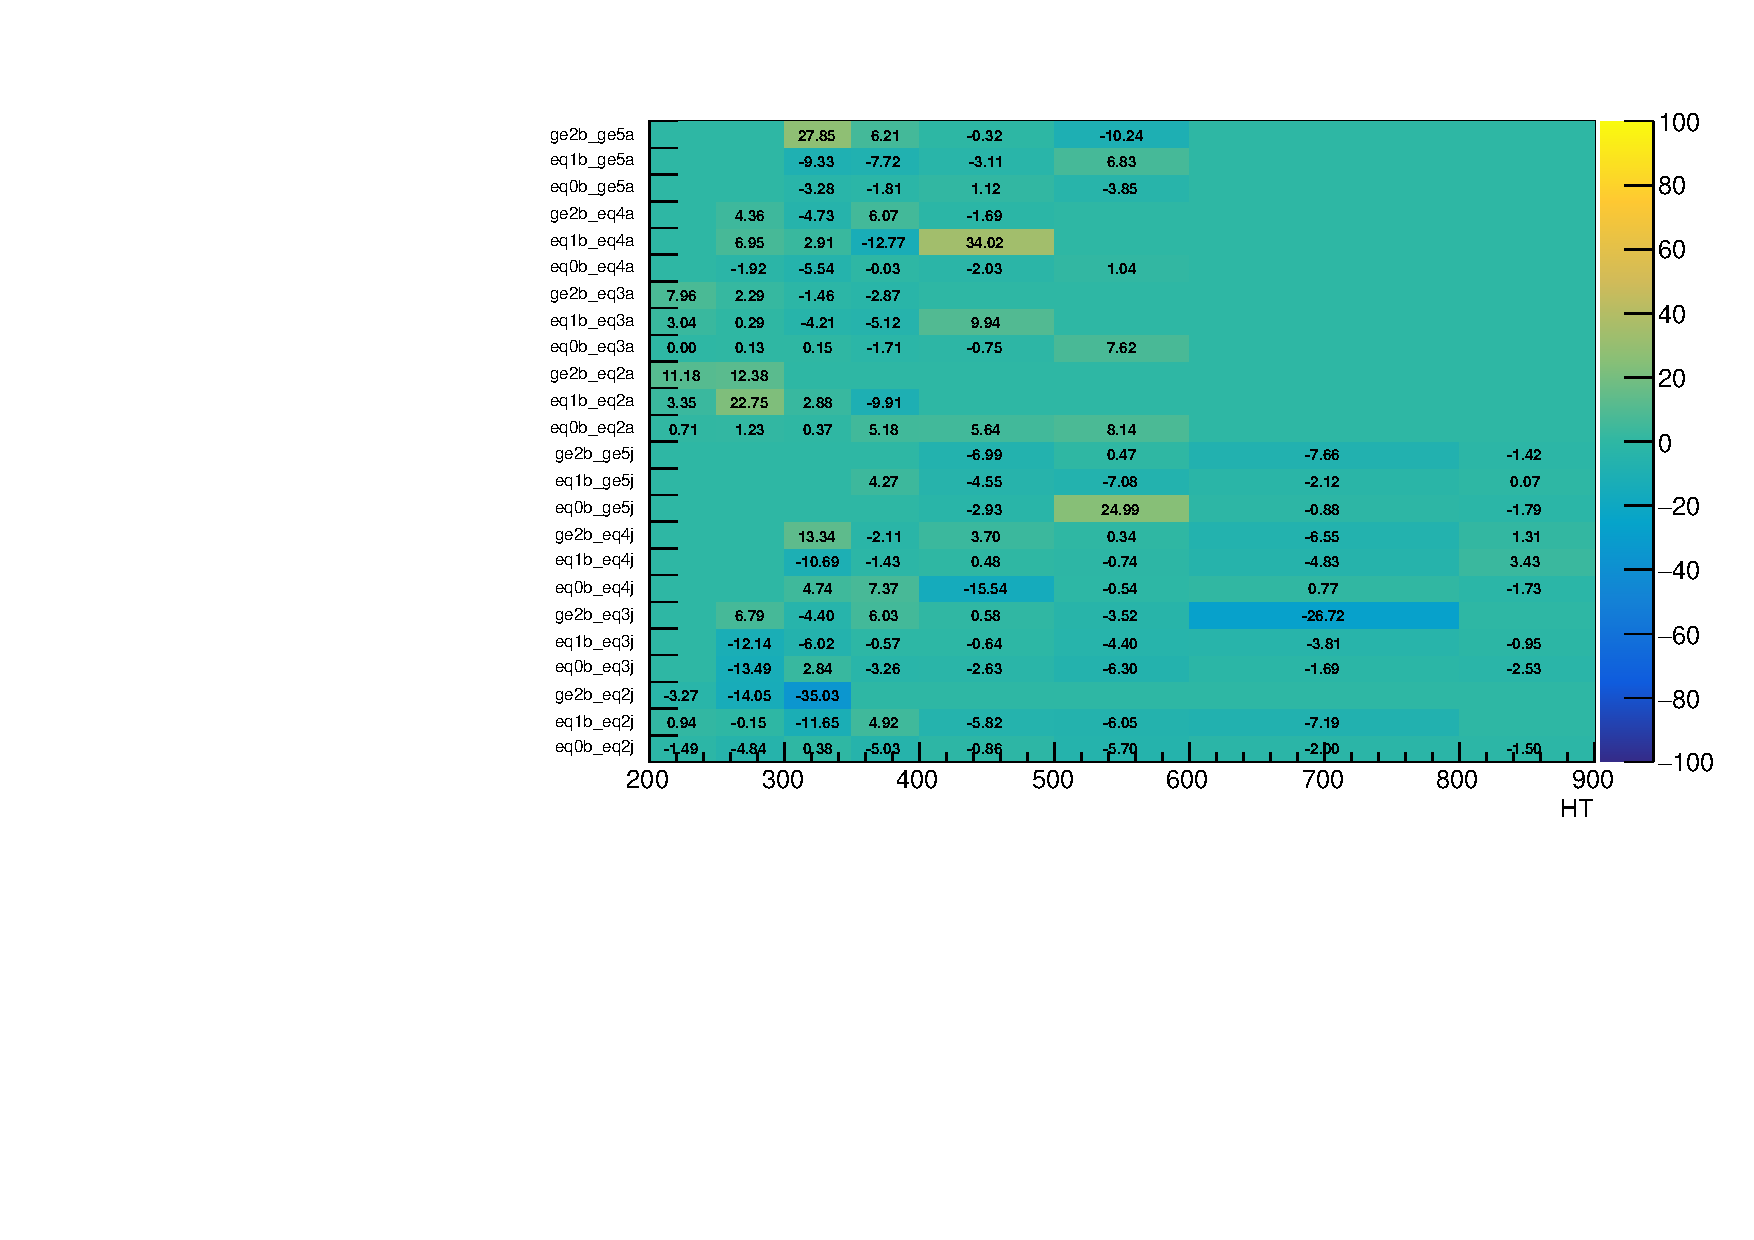
\includegraphics[width=0.5\textwidth]{figures/jesSystematics/SingleMu_MC_TF_Comp.pdf}
  } ~~
  \subfigure[The relative change in transfer factors for every
  analysis bin with an \alphat cut, inclusive on b-tags]{
    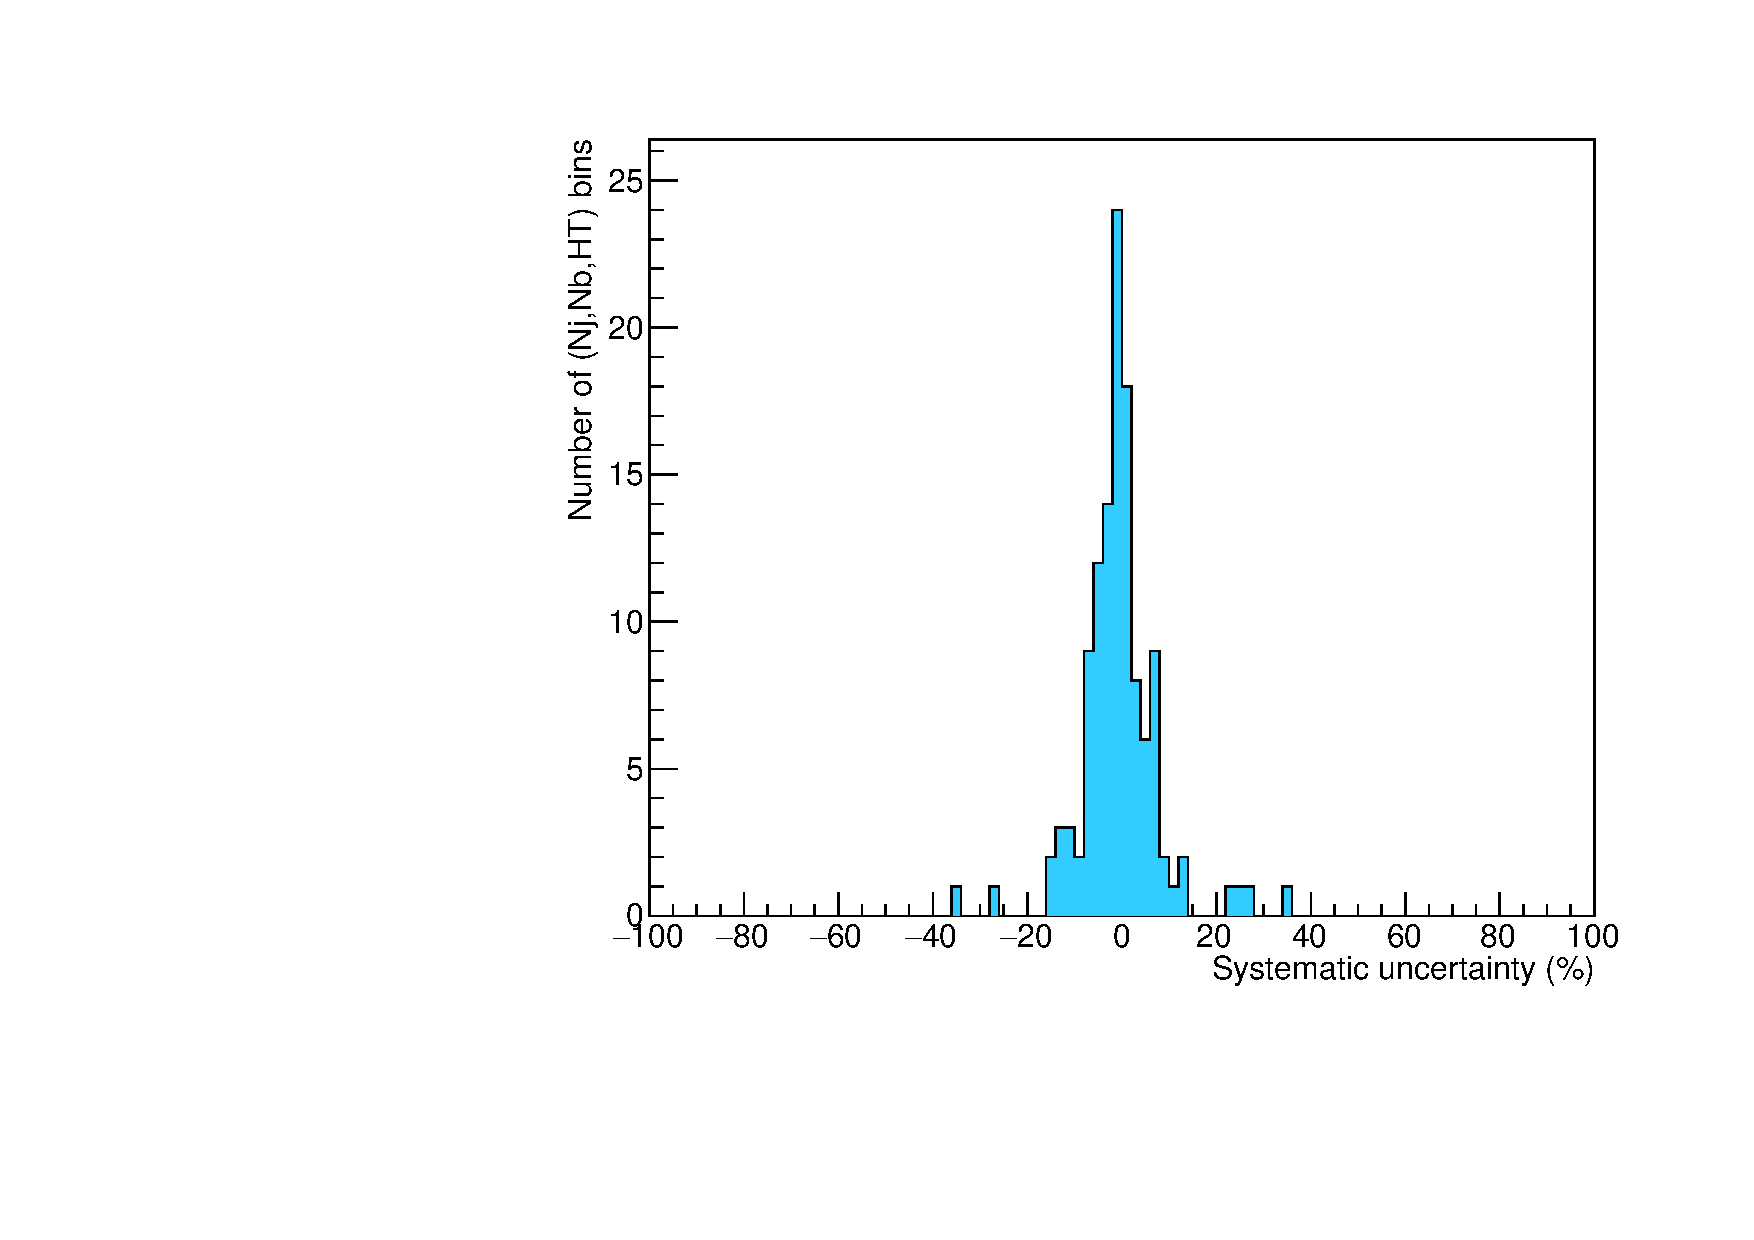
\includegraphics[width=0.5\textwidth]{figures/jesSystematics/SingleMu_MC_Systematics1D.pdf}
  }
  \caption{\label{fig:jes-syst-singleMu} The change in pseudo transfer
  factors when calculating them with nominal jet energy corrections
  and the minus one sigma level jet energy corrections in the \mj
  control sample.}
\end{figure}

\begin{figure}[]
  \centering
  \subfigure[The relative change in transfer factors per \scalht bin
  and jet category]{
    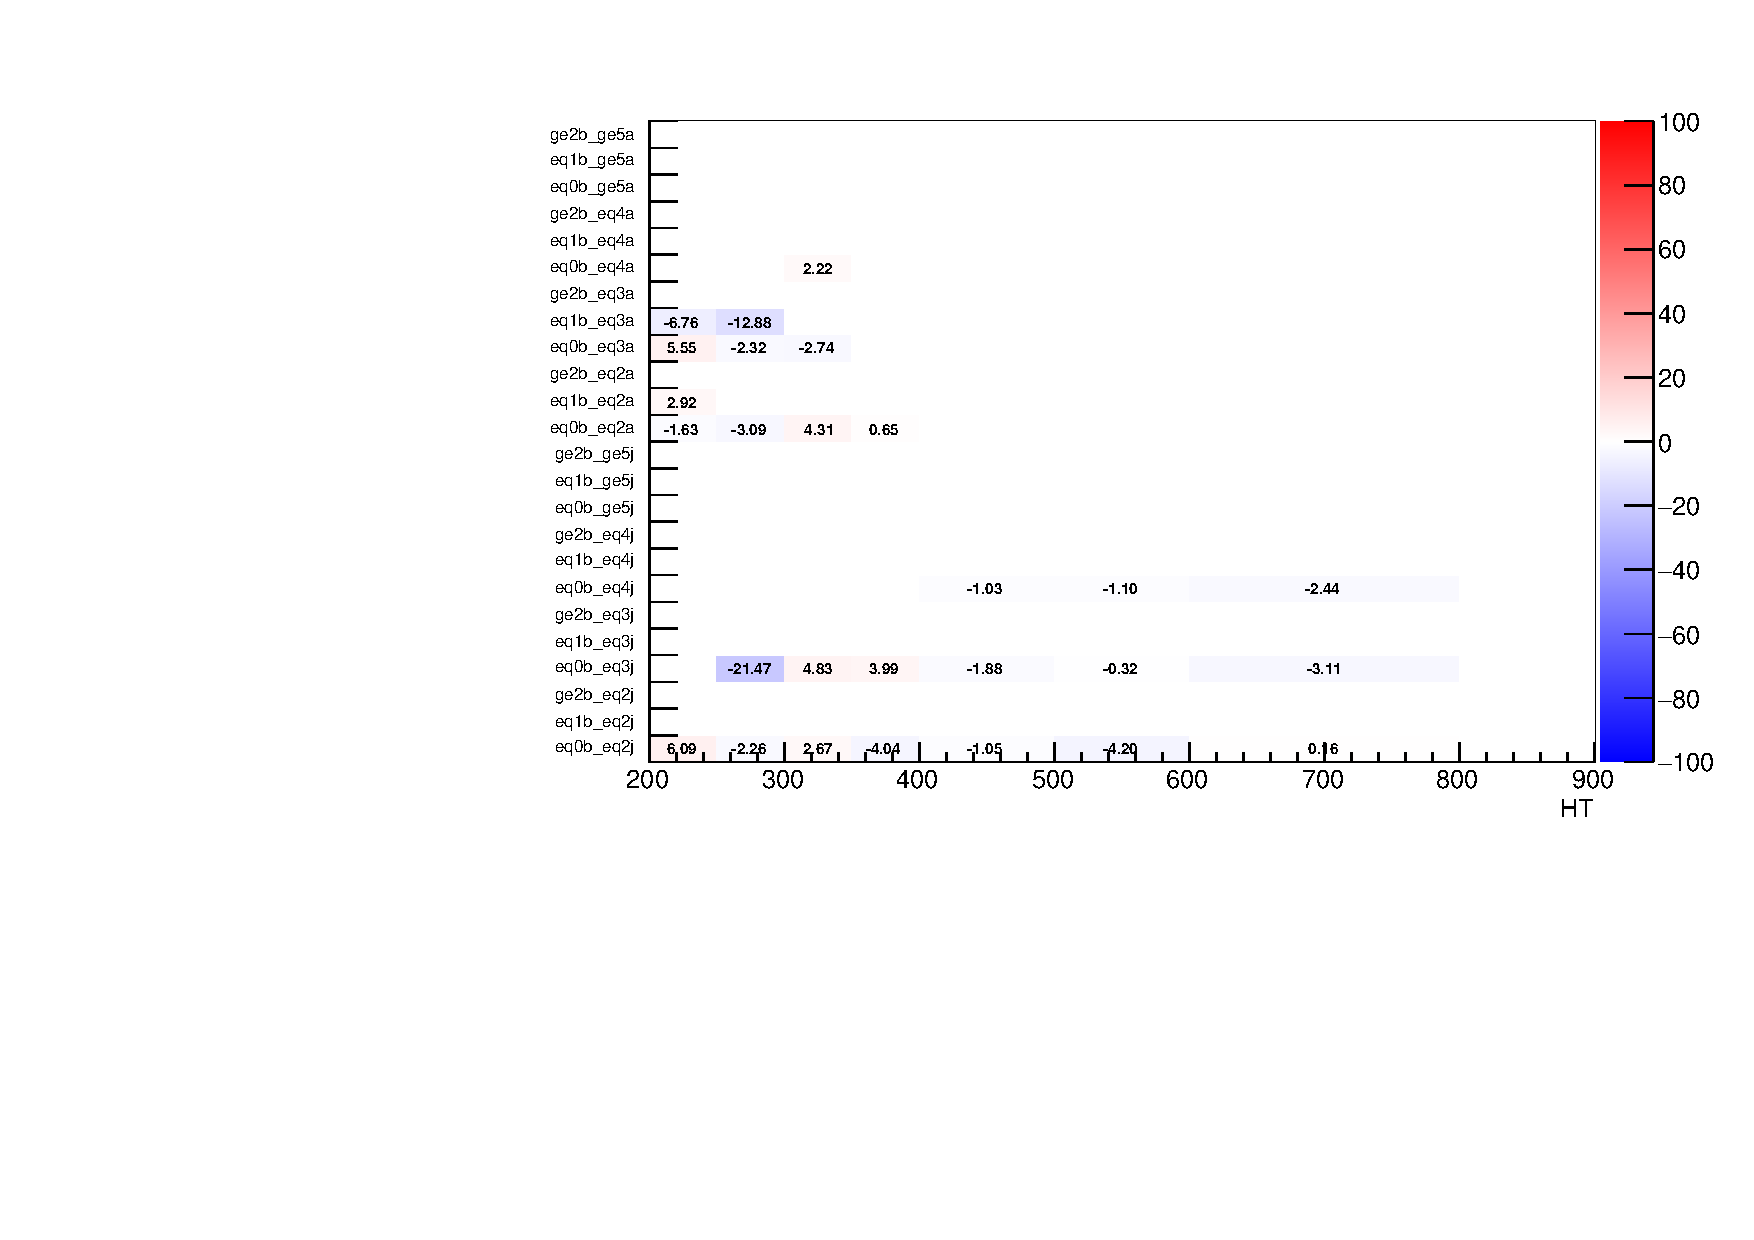
\includegraphics[width=0.5\textwidth]{figures/jesSystematics/DoubleMu_MC_TF_Comp.pdf}
  } ~~
  \subfigure[The relative change in transfer factors for every
  analysis bin with an \alphat cut, inclusive on b-tags]{
    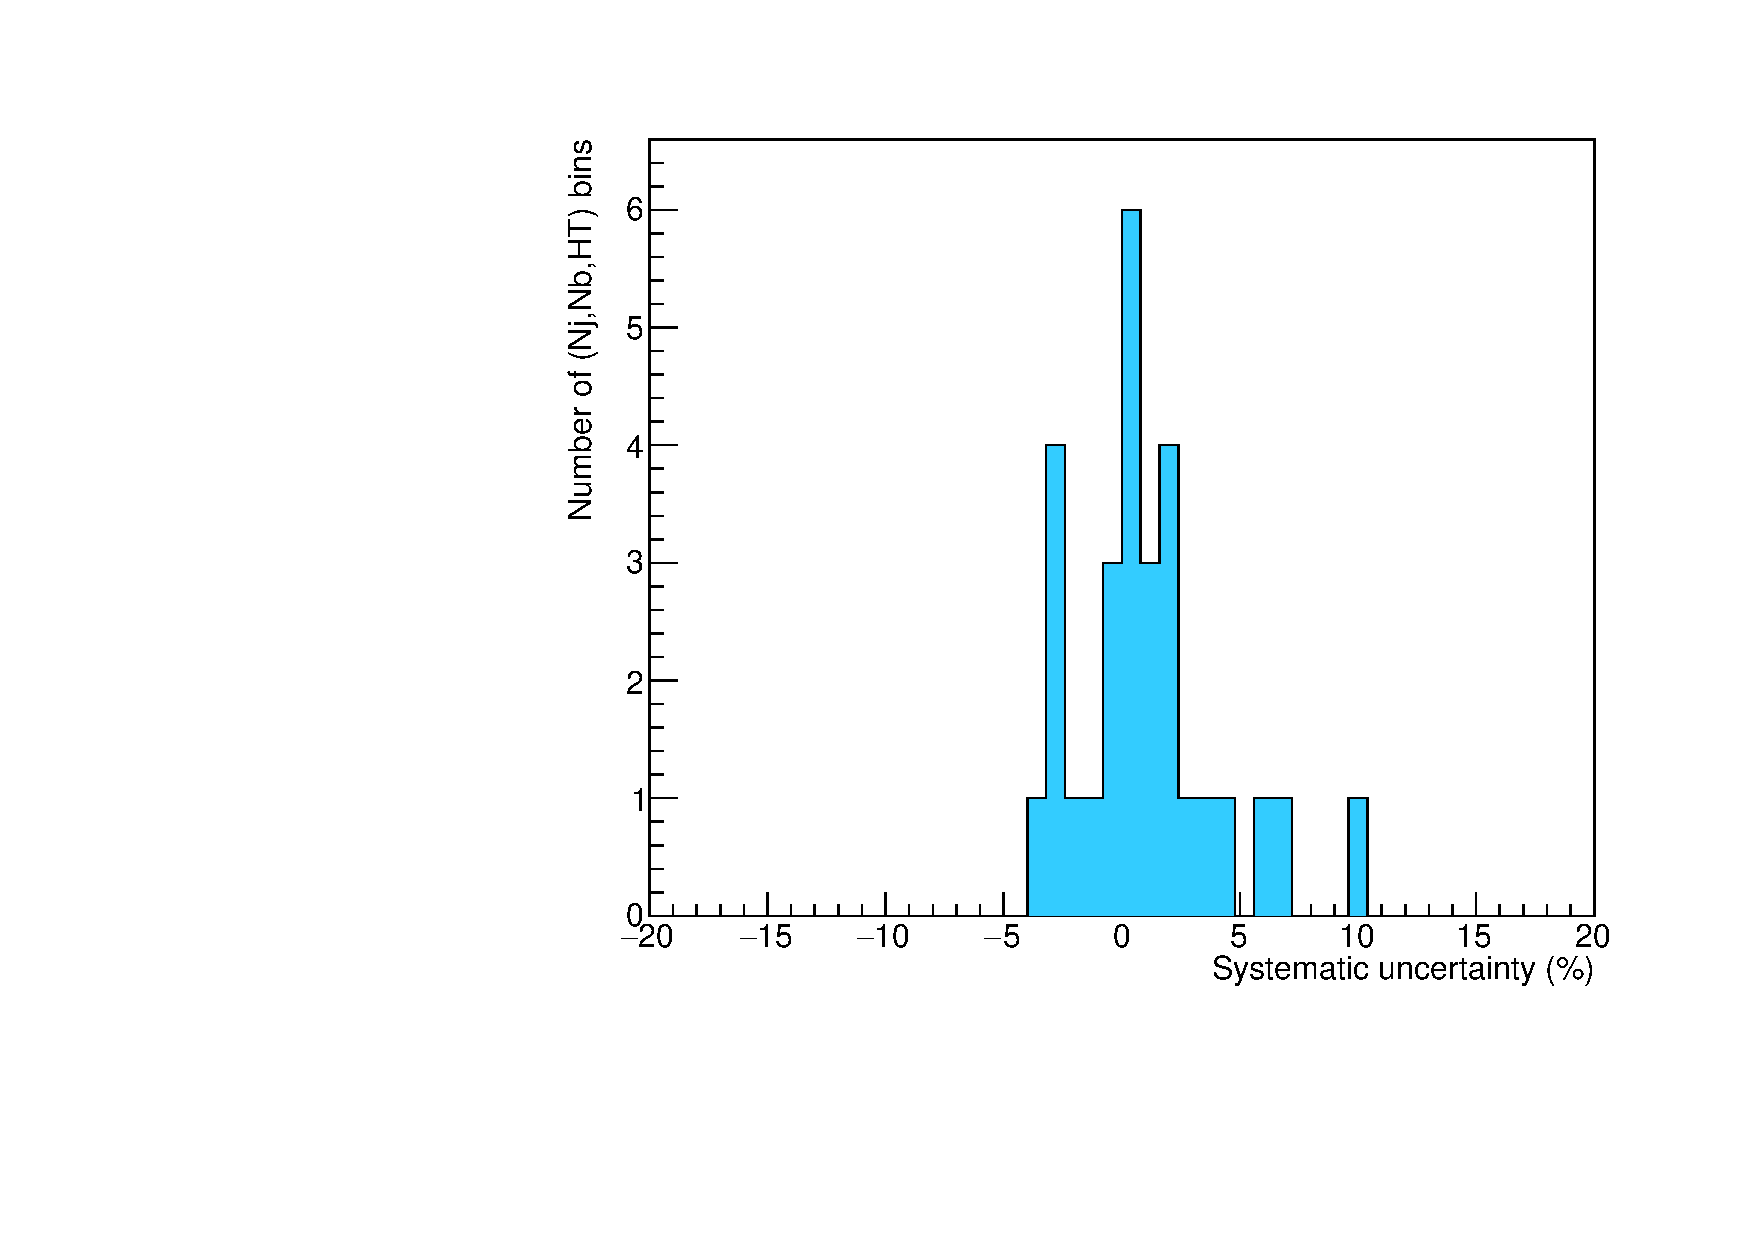
\includegraphics[width=0.5\textwidth]{figures/jesSystematics/DoubleMu_MC_Systematics1D.pdf}
  }
  \caption{\label{fig:jes-syst-doubleMu} The change in pseudo transfer
  factors when calculating them with nominal jet energy corrections
  and the minus one sigma level jet energy corrections in the \mmj
  control sample.}
\end{figure}


A check has also been performed on the systematic effect on the background 
prediction due to QCD contamination in the control samples, which has been found
to be at the percent level for the \mj and \gj control regions. Applying an
aribtrarily large variation of $\pm 100\%$ on the number of Monte Carlo QCD
events leads to a systematic variation on the transfer factors of at most 5\% in
the majority of bins.

These preliminary studies suggest that the jet energy scale and QCD
uncertainties are small and should be covered by the systematics derived from the
closure tests in Sec.~\ref{sec:closure-data-study}. The closure tests are
therefore a conservative estimate to which it can be established, based on data, 
that there is no significant bias in the background predictions. A more thorough 
study of these and additional source of systematic uncertainty will be carried 
out in the near future. If not sub-dominant, these additional uncertainties will
be propagated through to the final total.

% To be included at the end:
%Finally, an additional dedicated study is used to determine the
%systematic uncertainties that arise from uncertainties in scale factor
%corrections related to b-tag modelling. These are generally found to
%be small, at the percent level, and are typically sub-dominant with
%respect to the systematic uncertainties derived from the closure
%tests. However, if not sub-dominant, these additional uncertainties
%are propagated through to the final total.

